%loads the class that provides the titlepage and some general packages.
\documentclass{UniVieCS_Thesis} 

%add the additional packages and macros that you want to use
%here you can find some useful additional packages and macros

%Package to show algorithms
\usepackage{algorithm2e}

%package to work with glossaries
\usepackage[acronym]{glossaries}

%packages and setings to show colored code
\usepackage{listings}
\usepackage{xcolor}

\definecolor{codegreen}{rgb}{0,0.6,0}
\definecolor{codegray}{rgb}{0.5,0.5,0.5}
\definecolor{codepurple}{rgb}{0.58,0,0.82}
\definecolor{backcolour}{rgb}{0.95,0.95,0.92}

\lstdefinestyle{mystyle}{
    backgroundcolor=\color{backcolour},   
    commentstyle=\color{codegreen},
    keywordstyle=\color{magenta},
    numberstyle=\tiny\color{codegray},
    stringstyle=\color{codepurple},
    basicstyle=\ttfamily\footnotesize,
    breakatwhitespace=false,         
    breaklines=true,                 
    captionpos=b,                    
    keepspaces=true,                 
    numbers=left,                    
    numbersep=5pt,                  
    showspaces=false,                
    showstringspaces=false,
    showtabs=false,                  
    tabsize=2
}

\lstset{style=mystyle}

%package to allow comments/notes by you and other people
\usepackage[multiuser,marginclue,nomargin,inline,index]{fixme}
\definecolor{ttwgreen}{RGB}{75,135,73}
\fxusetheme{colorsig}
%\FXRegisterAuthor{tm}{atm}{\color{red}TM}
\FXRegisterAuthor{ttw}{attw}{\color{ttwgreen}TTW} % creates ttwnote, ttwwarning, ttwerror, ttwfatal commands
%\FXRegisterAuthor{mk}{amk}{\color{blue}MK}

%add your own packages or macros here

% important update for glossaries, before document 
\loadglsentries{C) Back Matter/acronyms.tex}
\loadglsentries{C) Back Matter/glossary.tex} 
\makeglossaries %https://www.overleaf.com/learn/latex/glossaries

%shows fixme notes
%\fxsetup{status=draft} % comment/delete this line if you want to your final output

\usepackage[ngerman, british]{babel} %if changed to \usepackage[ngerman]{babel} "Table of contents" changes to "Inhaltsverzeichnis", "abstract" becomes "Zusammenfassung" and "references" is translated to "Literatur".


%remove all the things you don't need and add all the things you need. you can also change the order of the elements at your will.
\begin{document}

    %Start with front matter
    
    %Choose the titlepage you want to use
    
    % --CHANGE THE TITLEPAGE HERE

% title page provided in Word by the University which can be found here 
% https://informatik.univie.ac.at/studium/hilfe-fuer-studierende/wegweiser-masterstudium/approbation-der-masterarbeit/ 
% Please pay attention to the guidelines that can be found there!
%


% There are some commands also for multiple lines. If something exceeds more than a line use the multi line commands. In the worst case adjust the vertical spaces within the class.
% -- Title Page
\Title{Graph algorithms for alchemical transformations using the free energy package Transformato} 
% A title exceeding one line can be created using the \TitleTwo or \TitleThree command
%\TitleTwo{I wish I \\ had a Master's Degree}
%\TitleThree{I wish I \\ had a Master's \\ Degree}
\Who{ Josef Anna Leopold Hackl, BA BA BSc BSc MA} %Make sure you add all your titles! 
% A name exceeding one line can be created using the \WhoTwo command
%\WhoTwo{ FirstName \\ LastName BSc}
\Degree{Master of Science (MSc)}
\Year{2023}
\ProgrammeCode{066875}
\ProgrammeName{Masterstudium Bioinformatik} %Make sure it has the same Name as in the Studienblatt
\Supervisor{Univ.-Prof. Mag. Dr. Stefan Boresch}
%\SupervisorTwo{Second Row} % Here you can change the row under the supervisor
%\CoSupervisor{0} %remove this line if there is a Co supervisor
\CoSupervisor{Dr. Marcus Wieder, MSc MSc}
%\CoSupervisorTwo{Second Row} % Here you can change the row under the cosupervisor

\Titlepage %This generates the titlepage %Creates the titlepage
    %% --CHANGE THE TITLEPAGE HERE

% title page provided in Word by the University which can be found here 
% https://informatik.univie.ac.at/studium/hilfe-fuer-studierende/bachelorarbeit-empfehlungen/ 
% Please pay attention to the guidelines that can be found there!
% If you want you can always create the titlepage in Word and then add it with \includepdf{<filename>} from the pdfpages package to your thesis.
%


%Do not change or delete the following two lines
\renewcommand{\TitleSetup}{BACHELORARBEIT / BACHELOR'S THESIS}
\renewcommand{\TitleTitleSetup}{Titel der Bachelorarbeit / Title of the Bachelor's Thesis\par}
% Change the rest of the lines to fit you thesis

% There are some commands also for multiple lines. If something exceeds more than a line use the multi line commands. In the worst case adjust the vertical spaces within the class.
% -- Title Page
\Title{I wish I had a Bachelor's Degree} 
% A title exceeding one line can be created using the \TitleTwo or \TitleThree command
%\TitleTwo{I wish I \\ had a Bachelor's Degree}
%\TitleThree{I wish I \\ had a Bachelor's \\ Degree}
\Who{ FirstName LastName } %Make sure you add all your titles! 
% A name exceeding one line can be created using the \WhoTwo command
%\WhoTwo{ FirstName \\ LastName }
\Degree{Bachelor of Science (BSc)}
\Year{2019}
\ProgrammeCode{126489}
\ProgrammeName{Masterstudium Informatik} %Make sure it has the same Name as in the Studienblatt
\Supervisor{Univ. Prof. My favorite professor, PhD}
%\SupervisorTwo{Second Row} % Here you can change the row under the supervisor
\CoSupervisor{0} %remove this line if there is a Co supervisor
\CoSupervisor{Professor Co}
\CoSupervisorTwo{Second Row} % Here you can change the row under the cosupervisor

\Titlepage %This generates the titlepage %Creates the titlepage
    %% --CHANGE THE TITLEPAGE HERE

% title page provided in Word by the University which can be found here 
% https://doktorat.univie.ac.at/doktoratsablauf/abschlussphase/einreichen-und-begutachtung/
% Please pay attention to the guidelines that can be found there!
% If you want you can always create the titlepage in Word and then add it with \includepdf{<filename>} from the pdfpages package to your thesis.
%


%Do not change or delete the following two lines
\renewcommand{\TitleSetup}{DISSERTATION / DOCTORAL THESIS}
\renewcommand{\TitleTitleSetup}{Titel der Disseratation / Title of the Doctoral Thesis\par}
% Change the rest of the lines to fit you thesis


% There are some commands also for multiple lines. If something exceeds more than a line use the multi line commands. In the worst case adjust the vertical spaces within the class.
% -- Title Page
\Title{I wish I had a Doctor's Degree} 
% A title exceeding one line can be created using the \TitleTwo or \TitleThree command
%\TitleTwo{I wish I \\ had a Doctor's Degree}
%\TitleThree{I wish I \\ had a Doctor's \\ Degree}
\Who{ FirstName LastName MSc} %Make sure you add all your titles! 
% A name exceeding one line can be created using the \WhoTwo command
%\WhoTwo{ FirstName \\ LastName MSc}
\Degree{Doctor of Philosophy (PhD)}
%\Degree{Doktorin ODER Doktor der >Zusatz< (Dr. >Abkürzung<)}
%\Degree{Doktorin OR Doktor der >affix< (Dr. >abbr.<)}

\Year{2019}
\ProgrammeCode{A 786 880}
\ProgrammeName{Doctoratsstudium Informatik} %Make sure it has the same Name as in the Studienblatt
\Supervisor{Univ. Prof. My favorite professor, PhD}
%\SupervisorTwo{Second Row} % Here you can change the row under the supervisor
\CoSupervisor{0} %remove this line if there is a Co supervisor
\CoSupervisor{Professor Co}
\CoSupervisorTwo{Second Row} % Here you can change the row under the cosupervisor

\Titlepage %This generates the titlepage %Creates the titlepage
    
    \clearpage
	\frontmatter{}

	%		%Please consider the following section of the "Formvorschriften für die gedruckte Version"
	%Im Anhang ist eine Zusammenfassung (Abstract) mitzubinden. 
	%Ist die Arbeit in einer Fremdsprache verfasst, ist im Anhang jedenfalls eine deutsche Zusammenfassung mitzubinden.
\chapter{Abstract}
		This \LaTeX{} template provides example on how to format and display text, 
		mathematical formulas, and insert tables or images. There is a lot more you 
		can do with \LaTeX{}, for more information check out https://en.wikibooks.org/wiki/LaTeX.
 % adds the abstract
	%\chapter{Kurzfassung}
Das ist eine deutsche Kurzfassung meiner in Englisch verfassten Masterarbeit.
\clearpage %adds the "Kurzfassung"in german.
	\pagebreak
	
    \microtypesetup{protrusion=false}
    \tableofcontents{}
    % Use an optional list of tables / figures / algorithms / listings(code).
    %\listoftables 
    %\listoffigures
    
    %\cleardoublepage{}
    %\listofalgorithms
    %\addcontentsline{toc}{chapter}{List of Algorithms} 
    %\cleardoublepage{}
    %\lstlistoflistings
    \cleardoublepage{}
    \microtypesetup{protrusion=true}
    
	\pagebreak
	
	%add your chapters here
	\mainmatter{}
	\chapter{Introduction}

The aim of this Master Thesis is to facilitate the preparation of
alchemical free energy calculations. Such calculations
estimate free energy differences by using unphysical intermediates, i.e. structures
which are not found in nature as existing chemical species. In addition
to the computation of absolute solvation and binding free energy differences,
the method can be used to compute relative free energy differences, e.g.,
the free energy difference of binding between two ligands. A problem occurring
in the latter approach is the need for so-called \textquoteleft dummy
atoms\textquoteright . Usually, the number of atoms between the two
end states, i.e., the two molecules of interest, is not the same.
However, this is a necessary condition for the molecular dynamics
simulations on which the computation of the free energy differences
is based. To preserve the number of atoms these dummy atoms act as
placeholders\cite{Fleck.2021, Karwounopoulos.2022}.

This Master Thesis is concerned with specific methods of handling these unphysical
atoms. A central part is the implementation of new features
for Transformato, a package which helps to set up relative alchemical
free energy calculations using an innovative common core approach\cite{key-2, Wieder.2022}.
In particular, helper functions are developed which optimize the employment of
the aforementioned dummy atoms. 
The implemented functions are collected in the  Python package tf-routes available on Github (https://github.com/jalhackl/tf\_routes/tree/master/tf\_routes).

In the following chapter, the basic principles of alchemical free energy
calculations are explained. The third chapter presents the workflow
of Transformato. Subsequently, the need for improving and extending some of the algorithms of the software
package is described in more detail. Examples for alchemical mutations
proposed by the new algorithms and corresponding common core constructions
for Transformato are given. Finally, the effect of different common core generation and mutation
algorithms on the results of free energy calculations is discussed.
	\chapter{Free Energy Calculations}

\section{Basics}

In the last few years, the accuracy and feasibility of free energy calculations
improved significantly \cite{King.2021}. The main reasons are developments
in the accuracy of force fields\cite{Cournia.2017}, the increase
in computational resources and, in particular, the usage of graphics
processing units to cope with the high computational demands. By now,
most MD software packages, like AMBER\cite{DavidA.Case.2005}, CHARMM\cite{Brooks.2009} or GROMACS\cite{Abraham.2015}, offer functions
for alchemical free energy calculations which facilitates the set-up
of such simulations. 

Possible applications can be found in rational drug design and drug
discovery; e.g., during lead optimization, the binding free energy differences
between compounds are of interest.\cite{Cournia.2017} As the free energy difference
 provides information about the thermodynamic favorability of a specific
process, it can help to find ligands that bind most tightly to a biomolecule of
interest.

One can distinguish between absolute and relative free energy calculations:
Absolute free energy differences are, for instance, solvation or binding
free energy differences of one compound (these results can be compared
with the free energy of an unrelated compound)\cite{Boresch.2003,Jorgensen.1988},
whereas the latter approach computes the free energy difference between,
e.g., two ligands, which usually are related to each other. For many
practical problems, such knowledge is sufficient, for instance, when
the comparison of properties like binding affinity of two ligands
is sought. The relative free energy differences between two ligands
can provide information to predict protein-ligand binding affinities
and to select specific ligands, drugs etc. for optimizing binding
affinity. Knowledge of binding affinities can be harnessed for tasks
like protein engineering \cite{King.2021}.

Relative free energy calculations harness the concept of a thermodynamic
cycle \cite{Kollman.}; see Fig.~\ref{fig:cycle}: The horizontal arrows indicate the
paths from the unbound to the bound state of each of the two ligands,
the vertical arrows indicate the transformation from one molecule
to the other one. According to the 2nd law of thermodynamics, the free energy differences along both paths
in the figure leading from the unbound state of ligand A to the bound state
of ligand B must be identical. In other words, we have
\[
\Delta G_{A}+\Delta G_{2}=\Delta G_{1}+\Delta G_{B}.
\]
From this one sees that the relative binding free energy difference between the two ligands can be expressed as \cite{Cournia.2017}:
\[
\Delta\Delta G=\Delta G_{2}-\Delta G_{1}=\Delta G_{B}-\Delta G_{A}.
\]
To obtain knowledge about $\Delta\Delta G=\Delta G_{B}-\Delta G_{A}$,
the evaluation of the alchemical transformations $\Delta G_{1}$and
$\Delta G_{2}$ suffices. (In practice, the determination
of $\Delta G_{A}$ or $\Delta G_{B}$ usually requires an experimental
set-up; thus, the alchemical calculation can substitute this step
or at least indicate if, e.g., a certain ligand is a promising candidate.)

The vertical part of the depicted thermodynamic cycle is easier 
to compute because the change between both states is much smaller
(depending on the molecules of interest, only some atoms change and hence there are fewer annihilation or creation steps) and, thus, in general, fewer intermediate steps
are necessary; however it involves 'alchemical' transformations, i.e.,
nonphysical intermediates have to be used. 
\begin{figure}
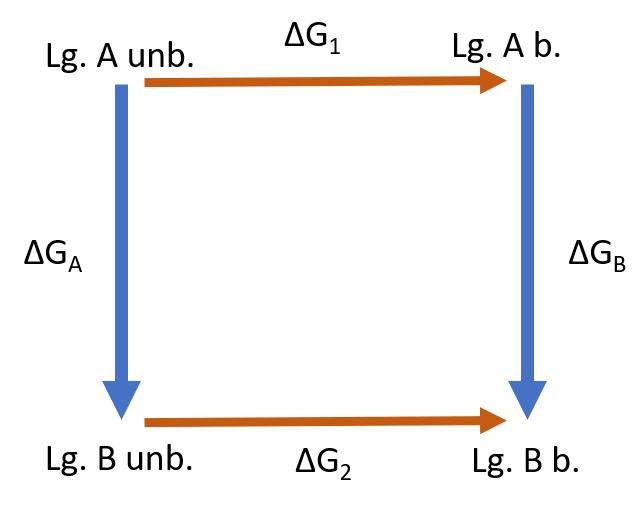
\includegraphics[scale=0.8]{cycle1}\caption{Thermodynamic cycle; red arrows indicate transitions between two states
(unbound--bound) of each ligand, blue arrows indicate 'alchemical'
transformations (Ligand~A--Ligand~B)\label{fig:cycle}}

\end{figure}

In general, the free energy is given by $F=-k_{B}T\ln Q$, where Q denotes the partition function $Q=\int dr\exp\left(-\beta U\right)$
with $\beta=\frac{1}{k_{B}T}$. Hence, the free energy difference between
states i and j can be described as \cite{Shirts.2013}:

\[
\bigtriangleup F_{ij}=-\frac{1}{\beta}\ln\frac{Z_{j}}{Z_{i}}.
\]

To compute the free energy differences between two states, various
methods exist. Usually, it is not possible to simply compute the difference
between the two end states; hence, intermediate states have to be taken
into account. The difference between the final states can be expressed
as the sum of the difference between these intermediate states: $\Delta F=F_{1}-F_{0}=\sum_{n}\Delta F_{n}$
\cite{Mey.2020}.

\section{Methods for evaluating free energy differences}

Various approaches for calculating free energy differences exist,
e.g., thermodynamic integration and perturbation. Implementations of the latter approach use
the Zwanzig formula or Bennett's acceptance ratio method (which is
used in the {\trafo} package described below). In the following,
these three approaches will be briefly outlined. (For a more
comprehensive comparison and estimation of performance differences,
see \cite{Bruckner.2011} and \cite{Ruiter.2013}).

\subsection{Thermodynamic Integration (TI)}

In Thermodynamic Integration, the free energy difference between two
states is computed by evaluating the integral over the derivative of the free energy
between the initial and the final state of the transformation/process studied. TI computes intermediate
states depending on the coupling parameter $\lambda$. $\lambda=0$
and $\lambda=1$ represent the physical, initial / final states of
the system. Scaling between those two values, i.e., using values $0\le\lambda\le1$,
gives rise to the nonphysical, 'alchemical' intermediate states.

Taking the derivative of the free energy, one gets $\frac{dF}{d\lambda}=\frac{d}{d\lambda}\int e^{-\beta U dr}=\left\langle \frac{dU\left(r,\lambda\right)}{d\lambda}\right\rangle _{\lambda}$\cite{Shirts.2013}, 
where the angular brackets indicate the ensemble average.
The free energy difference is then given as the integral from $\lambda=0$ to $\lambda=1$:
\[
\Delta F=
\intop_{\lambda=0}^{\lambda=1}\frac{dF\left(\lambda\right)}{d\lambda}d\lambda=
\intop_{\lambda=0}^{\lambda=1}\left\langle\frac{\partial U\left(\lambda\right)}{\partial\lambda}\right\rangle_\lambda d\lambda
.
\]
This integral has to be approximated using numerical integration, i.e., $\Delta F\approx\sum_{i}w_{i}\left\langle \frac{dU\left(r,\lambda\right)}{d\lambda}\right\rangle _{\lambda_{i}}$.
The weights $w_{i}$ depend on the choice of the numerical quadrature scheme.
A popular and simple choice is the trapezoidal rule, which uses equal
spacing between states and approximates the integral by $\intop_{\lambda=j}^{\lambda=i}\frac{dF\left(\lambda\right)}{d\lambda}d\lambda\approx\frac{i-j}{2}\left(f_{i}+f_{j}\right)$.
The integration scheme and the amount of intermediate steps has to
be chosen in such a way that the introduced bias is below the statistical
noise\cite{Shirts.2013}. (For a comparison of various numerical quadrature
schemes, e.g., the trapezoidal rule and Simpson's rule, see \cite{Bruckner.2011b}). 

\subsection{Free Energy Perturbation / Zwanzig Relation}

Free energy perturbation relies on the Zwanzig relation (or exponential
formula). For each configuration of state A, the energy difference
between this state and the corresponding state B is calculated, which is then used to compute the free energy difference between A and B according to \cite{Gapsys.2015}
\[
\Delta F_{A\rightarrow B}=F_{B}-F_{A}=-\frac{1}{\beta}\ln\frac{Q_{B}}{Q_{A}}=-k_{b}T\ln\left\langle \exp\left(\frac{-\Delta U_{A\rightarrow B}}{k_{B}T}\right)\right\rangle _{A}.
\]

Several variants of the formula exist: For instance, one can either
calculate forward or backward perturbations (either $\Delta F\left(A\rightarrow B\right)$ or
$-\Delta F\left(B\rightarrow A\right)$), or, as it is
usually the case, use double-wide sampling where energy differences
from both directions are processed \cite{Bruckner.2011}.

As for thermodynamic integration, usually it is necessary to
introduce intermediate states. The free energy between the final states
0 and 1 is calculated as the sum of the differences between all adjacent
intermediate states; in the case of n states: $\Delta F_{0\rightarrow1}=\sum_{i=0}^{n-1}\left(F\left(i+1\right)-F\left(i\right)\right)$.
There has to be a sufficient number of intermediate states --- there must be significant overlap between the two states --- otherwise convergence is poor.
However, there are still use cases when other methods are not feasible\cite{Boresch.2017},
and there exists an extension to non-equilibrium work (Jarzynski's
equation)\cite{Boresch.2017}. In general, however, it should be only used
if the difference between the two states are tiny\cite{Shirts.2013}.

\subsection{Bennett Acceptance Ratio (BAR)}

An extension of the perturbation approach for computing the free energy difference between
two states is Bennett's Acceptance Ratio\cite{Bennett.1976}. 

Expansion of the denominator and numerator of the ratio of the canonical
partition functions of both states leads to: 
\[
\frac{Q_{0}}{Q_{1}}=\frac{Q_{0}\int W\exp\left(-U_{0}-U_{1}\right)dq^{N}}{Q_{1}\int W\exp\left(-U_{0}-U_{1}\right)dq^{N}}=\frac{\left\langle W\exp\left(-U_{0}\right)\right\rangle _{1}}{\left\langle W\exp\left(-U_{1}\right)\right\rangle _{0}}
\]
where W denotes a (for now arbitrary) weighting function. Assuming
a Gaussian distribution of the estimation error in the limit of large
samples, the optimal W can be determined as $W\left(q_{1}...q_{n}\right)=c\left(\frac{Q_{0}}{n_{0}}\exp\left(-U_{1}\right)+\frac{Q_{1}}{n_{1}}\exp\left(-U_{0}\right)\right)^{-1}$\cite{Bennett.1976}. 

To use Bennett's acceptance ratio method, two simulations have
to be carried out. One starts at $\lambda=0$, the other one at $\lambda=1$.
Forward and backward simulations are processed simultaneously. 

The free energy difference between two $\lambda$-states can be expressed as
\[
\bigtriangleup F\left(\lambda_{i}\rightarrow\lambda_{j}\right)=\beta^{-1}\left(\ln\frac{\left\langle f\left(U_{\lambda_{i}}-U_{\lambda_{j}}+C\right)\right\rangle _{\lambda_{j}}}{\left\langle f\left(U_{\lambda_{j}}-U_{\lambda_{i}}+C\right)\right\rangle _{\lambda_{i}}}\right)+C
\]
with the Fermi function $f\left(x\right)=\frac{1}{1+\exp\left(\beta x\right)}$
\cite{Bruckner.2011,Gapsys.2015}.

To obtain the value of the optimum shift constant,
\[
C=\beta^{-1}\ln\frac{Q_{i}N_{j}}{Q_{j}N_{i}},
\]
a self-consistency
problem has to be solved iteratively\cite{Gapsys.2015}.

The free energy between two $\lambda$-states is then given by $\bigtriangleup F\left(\lambda_{i}\rightarrow\lambda_{j}\right)=\beta^{-1}\ln\frac{N_{j}}{N_{i}}+C$\cite{Bruckner.2011}.
$N_{j}$ and $N_{i}$denote the number of sampled configurations from
state j and i, respectively.

BAR gives a minimal variance free energy estimate. There is also an
alternative derivation for the formula. It can be shown that the
Bennett acceptance ratio method works as a maximum likelihood estimator.
Using BAR, one obtains the asymptotically unbiased estimation (i.e., for an infinite
number of measurements it yields an unbiased estimation) 
with the lowest variance\cite{Shirts.2003}. 

Using variational calculus to minimize the variance, $\Delta F$ can
be expressed implicitly as:$\frac{\partial\ln L\left(\Delta F\right)}{\partial\Delta F}=\sum\frac{1}{1+\exp\left(\beta\left(M+W_{i}-\Delta F\right)\right)}-\sum\frac{1}{1+\exp\left(\beta\left(M-W_{j}-\Delta F\right)\right)}=0$
, where M denotes $M=\beta^{-1}\ln\frac{N_{j}}{N_{i}}$ \cite{Shirts.2003}.

BAR also depends on the overlap between the states; however, it is
more robust and reliable in cases of rather poor overlap \cite{Ruiter.2013}
(especially when compared to FEP). (Whether BAR outperforms thermodynamic
integration crucially depends on the smoothness of the integrand.
For more pronounced changes in molecular properties between the computed
states, BAR seems to be superior\cite{Shirts.2013}.)

\section{Soft-core potentials}

Alchemical transformations rely on a coupling parameter $\lambda$ which
is used to gradually modify interactions. For example, by scaling $\lambda$, one can weaken the interaction with one part of the system and remove them completely at the final state. (In the simplest case,
there are only two states corresponding, e.g., to an atom present in
one of the two molecules but not in the other one. If the two molecules
have more considerable differences, this annihilation process has to be carried out for each atom, which has to be transformed
into a dummy atom.)
The term 'van der Waals endpoint problem' (or even 'catastrophe') denotes
several problems which can occur when a particle is removed (i.e.,
turned into a dummy atom by turning off its intermolecular interactions).
\cite{Boresch.2011}

We illustrate the types of problems, which can arise, for the case
of a linear dependence of the coupling parameter,
i.e.

\[
U\left(\lambda\right)=U_{o}+\lambda\sum_{1\leq i\leq N-1}u_{i,N}.
\]


(Of course, the equal spacing of the coupling parameter does not imply
equal phase-space overlap between the states \cite{Shirts.2013};
thus, for many simulations this simple set-up is certainly not the
optimal solution.) For $\lambda=0$ and $\lambda\approx0$ various
issues emerge. If $\lambda=0$, there are no interactions (and hence
no repulsion) and the non-interacting dummy particle can be located
at the exact position of another particle. This could give rise to
errors resulting from divisions by zero. (In contrast to the next two scenarios,
this seems to be a minor problem avoidable by efficient coding, i.e.,
implementing an additional clause for this condition to avoid the division by zero. In fact, it appears that all common MD
simulations packages manage this case automatically\cite{Boresch.2011}).

For $\lambda\rightarrow0$, numerical instabilities can occur because
even within a small time-step the interactions can become highly repulsive.
It should be noted that this problem emerges at values $\lambda\approx0$,
but not at $\lambda=0$ (i.e., when the particles are completely decoupled).

If thermodynamic integration is used, a related problem occurs because
$\left\langle \frac{\partial U}{\partial\lambda}\right\rangle _{\lambda}$can
become singular. This is obvious for the example using a linear pathway:
$\frac{\partial U\left(\lambda\right)}{\partial\lambda}=\sum_{1\leq i\leq N-1}u_{i,N}$.
As for the problem leading to a division by zero, the fact that one of the
still interacting particles can be located at the same place
in the simulation box as the dummy atom causes this quantity to change
unpredictably and, in the worst case, become singular \cite{Boresch.2011}.

The established way to avoid such problems is the usage of soft-core potentials \cite{Steinbrecher.2011}.
An additional term is added to the particle-particle distance in the Lennard-Jones potential so that
no division by 0 occurs and the corresponding derivative does not
become singular. The usual Lennard-Jones potential is replaced by
a slightly modified potential which ensures that at $r=0,\lambda>\text{0}$
the divisor is never 0 and the division by zero is avoided:

\[
U_{LJ}\left(r,\lambda\right)=\left(1-\lambda\right)\left(\frac{A}{\left(r^{2}+\lambda\delta\right)^{6}}-\frac{B}{\left(r^{2}+\lambda\delta\right)^{3}}\right)
\]

However, the usage of soft-core potentials has some limitations. In
particular, the availability of soft-core potentials depends on the
used software package. Free energy calculations have to be explicitly
supported. 

\section{Dummy atoms, Single/Dual topology}

Usually, the number of atoms of both molecules of interest, i.e., of the
two end states of an alchemical free energy calculation, is not
the same. However, the atom number has to stay constant (as the simulation
takes place in the canonical ensemble). Because of that constraint,
so-called dummy atoms are necessary \cite{Fleck.2021}. These dummy
atoms do not participate in any non-bonded interactions, but they
have to be connected via bonded interactions to the rest of the molecule
they belong to so that they do not get detached and float through
the simulation box.

There are two main approaches for setting up alchemical mutations, both involving dummy atoms: 

In single topology, during the mutation process, physical atoms, which belong only to the start state, are
transformed into dummy atoms at the end state. Conversely, 
as the alchemical transformation proceeds, dummy atoms present at the initial state are re-transformed
into physical atoms of the second molecule.

In dual topology, no direct mutation of real atoms into dummy atoms
occurs. However, both physical molecules are augmented with all dummy
atoms of the respective other state (hence, there is no state during the simulation
without dummy atoms). Thus, the number of dummy atoms equals the number
of atoms which have no direct correspondence in the other molecule.
Usually, in total, even more dummy atoms are present in the system
as in a single topology setup \cite{Fleck.2021}.

The implementation of such dummy atoms, however, is not without pitfalls.
In single topology, errors can arise if too many bonded interactions are kept. The order in which interactions are turned off has to be constrained
by specific rules to ensure that the contributions exactly cancel
out each other, and attention has to be paid to under which conditions
dummy atom contributions cancel out exactly. \cite{Fleck.2021}

\section{Serial atom insertion}

As an alternative to modifying the coupling parameter, one can
try to create new states by turning off atoms in one step without
intermediate values. In \cite{Boresch.2011}, this approach is called
Serial atom insertion. Atoms are turned off serially (one after one
or in small batches). There is no gradual damping of the interactions; the
LJ-interactions of a molecule are either present ( $\lambda=1$) or
turned off ( $\lambda=0$).

A sufficient overlap of neighboring states in phase space is crucial
for any alchemical free energy calculation. So the question arises
if turning off of one atom in one step is in agreement with this prerequisite. The feasibility of this approach relies on Bennett's acceptance
ratio which was shown to work with neighboring states created
by serial atomic insertion \cite{Boresch.2011}.

In particular, Serial atom insertion has the advantage that it works
even for MD algorithms which lack explicit support for free energy
simulations and soft-core potentials are not needed (because the coupling
parameter takes only the values 0 and 1). The free energy differences
between states can be assembled from 'normal' simulations.

The most severe restriction due to the van der Waals Endpoint
problem is the instability of the integrator near the endstate where an atom has almost vanished (i.e.,  $\lambda=0$ or  $\lambda=1$). As such states
are not used in Serial atom insertion, this problem is automatically
avoided.

The feasibility of this approach depends on the sufficient overlap
between the states. Using BAR, no intermediate steps are necessary
and atoms can be turned off one by one. Contrariwise, thermodynamic
integration cannot be used because it is exactly the scaling of the
interaction parameter between 0 and 1 which is avoided. This also
implies that the singularity risk of the derivative due to the van
der Waals endpoint problem can be neglected (as this part of the problem
only concerns thermodynamic integration).
	\chapter{{\trafo} }

{\trafo} uses a common core scaffold which contains the subset of atoms which are present in both molecules (i.e., a one-to-one correspondence between
atoms of both molecules, which in the test cases shown below is always
based on atom identity). Both initial states of the alchemical transformations initialized by {\trafo} do not contain any dummy atoms, but consist solely of the physical atoms of the respective molecules. However, dummy atoms are generated via two separate alchemical paths leading to the common core. Starting from the initial states, physical atoms are successively turned into dummy atoms until the common core structure is reached. 

In each transformation step, one physical atom (or, if phase space
overlap is sufficient, a batch of adjacent atoms) is changed into
a dummy atom (until the common core is attained).

The common core architecture circumvents some potential problems
associated with the single and double topology approaches for dummy
atoms. The physical end states of the molecules are mutated until the
common core structure is attained. This implies that both starting states
do not contain any dummy atoms (these states are identical to the
physical molecules of interest). Therefore, it is ambiguous if the
alchemical transformations implemented in {\trafo} rather belong
to the single or the dual topology paradigm: As in the latter, different
dummy atoms are generated for each molecule along the path to the
common core, but --- in contrast to the usual dual topology approach
--- the final states are free of any dummy atoms. 

The 'removal' of atoms, i.e., the mutation into dummy atoms, is performed
using the serial atom insertion approach described above; hence, {\trafo}
does not rely on the use of soft core potentials. The computation
of the resulting energy differences is based on MBAR.

Therefore, by setting up the mutation path between two molecules across
the connecting common core and using serial atom
insertion, the {\trafo} workflow is independent of the underlying
molecular dynamics package and of the availability of explicit free energy
calculation code. In principle, {\trafo} can work on top of every
molecular dynamics simulation package.

Input can be created via CHARMM-GUI\cite{Jo.2008}. The solution builder of the website generates appropriate files to run MD simulations for the systems for which free energy differences shall be determined (e.g., for relative solvation free energy differences, input files for both molecules in a water box and in vacuum).\cite{Braunsfeld., Karwounopoulos.2022}.

\section{Common core approach}

The main condition for the common core of two molecules is the existence
of a one-to-one correspondence of atoms, i.e., the existence of a graph
isomorphism. The {\trafo} workflow imposes some further conditions
on the properties of the common core:

The junction between the common core and dummy region has to be unique;
only one dummy region is allowed to be connected via one bond to the
common core. In particular, the maximum common substructure must not
encompass partial rings (which would imply that dummy regions are
connected via multiple bonds). (In general, such transformations can pose intricate problems because ring breakage can lead to fast changes in free energy
and cause significant estimation error \cite{Liu.2015}.)
To meet these requirements, adjusting of the parameters and algorithms for finding the common core is important. For facilitating the construction of appropriate common cores, it was also necessary to improve the processing of the hydrogen atoms. As hydrogens are turned off beforehand in one step and not via serial atom insertion like the heavy atoms, it would be  detrimental to consider them in the common core generation (see section 'Processing of hydrogen atoms' in the next chapter). In previous versions of {\trafo}, hydrogens were included in the common core generation steps, which led to small or often even completely infeasible common cores. Before the common core construction is carried out, hydrogens have to be
removed from the molecule representation. This is an important step
because the presence of hydrogen atoms can lead to a different common
core (which is created, using default settings, by maximizing the
number of corresponding atoms) and subsequently a suboptimal mutation
route. 




\section{{\trafo} workflow}


During the mutation process, the contributions of the non-CC atoms are turned off gradually; five stages can be discerned \cite{Karwounopoulos.2022}:  In the first step, the electrostatic interactions of dummy atoms are gradually turned off. Next, Lennard-Jones interactions of all hydrogen atoms outside the common core are removed. This can be carried out in a single step.
During the third stage, the LJ-interactions of the non-CC non-hydrogen atoms are processed. One atom per step is turned off following the serial atomic insertion approach. (Possibly, a small group of atoms could be turned off in one step, but it is not recommended to process more than two atoms at once to ensure sufficient phase space overlap between the states.)
The atom which connects the common core and the dummy region is  called the junction atom and indicated as 'X' \cite{Karwounopoulos.2022} (In the plots in the next chapters, for simplicity, the indication of the junction atom is sometimes omitted. However, it should be stressed that, e.g., a transformation to a methane common core yields, in fact, a $\mathrm{CH_3X}$ common core.). This dummy atom which is directly connected to the common core needs special treatment. In contrast to the other atoms of a dummy region, its LJ interactions are not turned off completely, though its partial charge has to be zero.\cite{Karwounopoulos.2022} This junction atom ensures that the double free energy differences are not influenced by contributions of dummy atoms.\cite{Fleck.2021}
In the last step, it has to be ensured that both common cores are identical, e.g., differences in charge distribution have to be adjusted and the bond between junction atom and the common core atom has to be identical.


	\chapter{Problem description }

The main objective was the assessment and improvement of some routines
used in the free energy package {\trafo}. A further goal was to
minimize the necessity of manual adjustments by the user, i.e.,
reasonable mutation routes should be generated automatically. The
proposed route should be directly usable for the further {\trafo}
workflow.

In a first step, the reliability of the current {\trafo} workflow
had to be assessed, for instance the quality of the proposed common
cores. Different settings for the construction of the maximum common
substructure were compared. 

The order of the transformation steps was optimized, especially
for the case of more complex mutation routes which occur for connected
dummy regions involving ring structures, multiple chains or different
atom types. 

Particularly intricate problems occur for ring structures. In contrast to a chain, which usually has only one possible mutation order without leading to disconnected components, multiple possibilities  exist for rings. (Because of this, the evaluation of the mutation algorithms in the following sections will focus on such transformations.) The mutation of atoms should neither generate vacancies in the inner part of the
molecule nor should rings remain opened longer than necessary, and
a sufficiently systematic and --- especially concerning rings --- symmetric
processing of the nodes has to be performed. These rules have to be
implemented by maintaining the crucial constraint that no atoms are
detached from the main part encompassing the common core, i.e., no
disconnected components must emerge under any circumstances.

Using a graph representation of the involved molecules, the construction
of the intermediates between the final states was optimized.
New algorithms were written in Python and subsequently integrated
into the existing {\trafo} package. Finally, the effect of different
algorithms on the efficiency of the free energy calculations was validated through molecular dynamics simulations. 

To obtain a reliable test set of molecules, sdf-files of ligands were downloaded from the PDBbind-CN database. These test molecules cover a
broad range in size, complexity and potentially intricate compounds,
like polycyclic structures and highly branched chains.

\section{Overview of algorithms and software packages used}

The {\trafo} package is written in Python. Therefore, Python packages
were also used for molecule processing and graph representations.
The creation of molecule objects and the determination of the maximum
common substructure is done via Rdkit\cite{key-3}. NetworkX\cite{AricA.Hagberg.2008}
provides functions for graph visualization and analysis. It is easy to convert molecules created using Rdkit into NetworkX graph-objects
and hence utilize the functions of NetworkX for the molecules and
common cores constructed. Particularly, graph traversal algorithms
like breadth-first and depth-first search can be easily implemented
(see below).

\section{Assessment of common core settings}

Rdkit allows the search for a maximal common substructure (which can
serve as the common core for {\trafo}) via the \texttt{rdFMCS.FindMCS}-function.
Per default, the objective is to maximize the number of atoms, albeit
different settings, like maximizing the number of bonds or ignoring
or equalizing specific atom types are available. Currently, for
{\trafo} maximization of atoms and atom identity is used. As stated above, the presence of hydrogens can influence
the maximum common substructure heavily (fig. 4.1) because the number of atoms is modified, and this quantity is maximized for the maximal common substructure. 

Settings concerning the allowed involvement of ring structures in
the common core are of crucial importance. Firstly, these parameters
can influence the common core construction drastically and, secondly, they
can even be decisive whether the generated common core is valid for the
{\trafo} workflow.
Especially for the generation of common cores for polycyclic molecules, e.g., sterols, these parameters are of utmost importance.  
Important ring-related settings are \texttt{ringMatchesRingOnly}, \texttt{completeRingsOnly}
and the \texttt{ringCompare-parameter}. 

To obtain valid common cores of molecules involving cyclic structures for the processing of {\trafo}, \texttt{ringMatchesRingOnly}
and \texttt{completeRingsOnly} must be set to True: The former argument indicates
that ring atoms of one molecule are only matched against ring atoms
of the other molecule, the latter ensures that no partial rings are
involved in the common core. Especially, the latter constraint is a
necessary condition for a valid common core. (Otherwise, if partial
rings take part of the common core, dummy regions will be inevitably
connected to the common core via multiple bonds.)

The \texttt{ringCompare}-parameter parameter accepts the \texttt{StrictRingFusion}-argument.
It imposes that in the case of multiple rings, aromaticity is properly
considered. Fig. 4.2 illustrates the effect of the parameters
on the common core of two cyclic example molecules. However, as shown in the bottom row of Fig.~4.2, enforcing
of \texttt{StrictRingFusion} can still lead to maximum common substructures
that are not valid {\trafo} common cores in case of a dummy region
which is connected via multiple ring atoms of the same ring with the common
core. 
When an invalid common core is generated, it appears to be advisable to warn the user in this case that the common core does not fit the expectations of the {\trafo} workflow. 
The mutation algorithms presented below can deal with such invalid common cores. A helper function arbitrarily chooses one of the connections between the common core and the dummy region, and the other ones are ignored for the mutation path. However, this only ensures that a mutation route is returned; the current {\trafo} workflow is not adapted to deal with such common cores properly. Therefore, it only makes sense for test purposes and may not provide a reasonable input for the regular workflow.
Alternatively, one could check after the creation if the common core is valid. If
it is not, one could for instance search for a new common core encompassing fewer
atoms until a valid common core is found (see below). A further option would be to prohibit the involvement of ring atoms for this particular molecule combination.

These problems occur because the requirements for a valid {\trafo} common core are stricter than the constraints imposed by rdkit  (even when all ring-related parameters are applied, i.e., \texttt{ringMatchesRingOnly}, \texttt{completeringsonly} and \texttt{strictringfusion}): For {\trafo}, is not only indispensable that the common core solely comprises complete rings, but also the molecule fragment consisting of the non-common core atoms (which implies that there is a unique connection between dummy region and common core).
An efficient and straightforward solution for this problem, which always yields the best --- i.e., largest --- valid common core if one exists, has been implemented:
The basic observation is that if common core atoms within a cyclic region give rise to an invalid common core, it is impossible that any atoms within this region could participate in a valid one (if this would be the case, the whole cyclic region would be already in the generated common core).
After generating a common core with standard parameters, it is checked if the additional requirements concerning the ring structure hold, i.e., if the non-common core atoms (as well as the common core atoms) of both molecules do not participate in a partial cycle.
(Alternatively, one could check if a path between the non-common core atoms adjacent to the common core, i.e., the X-atoms, exists. If this is the case, the common core obviously is not valid, since no unique atom which connects the common core and a specific dummy region is present.)





\begin{figure}
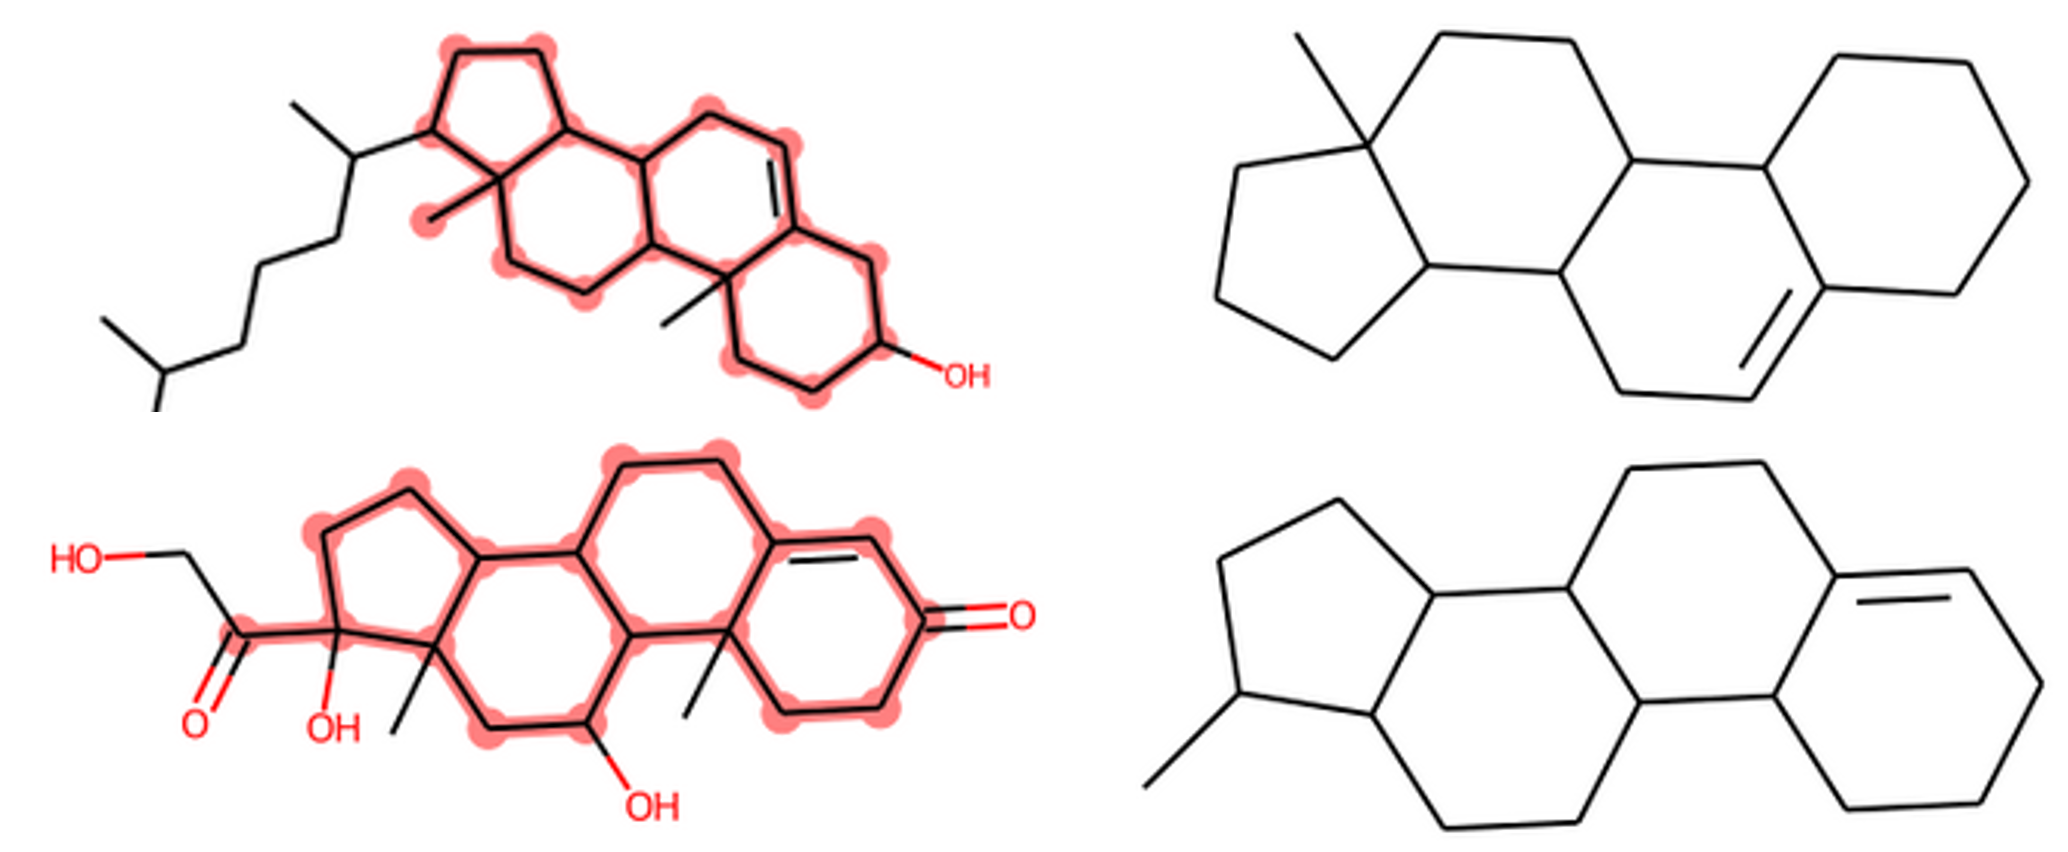
\includegraphics[scale=0.45]{sterols_wo_strictfusion}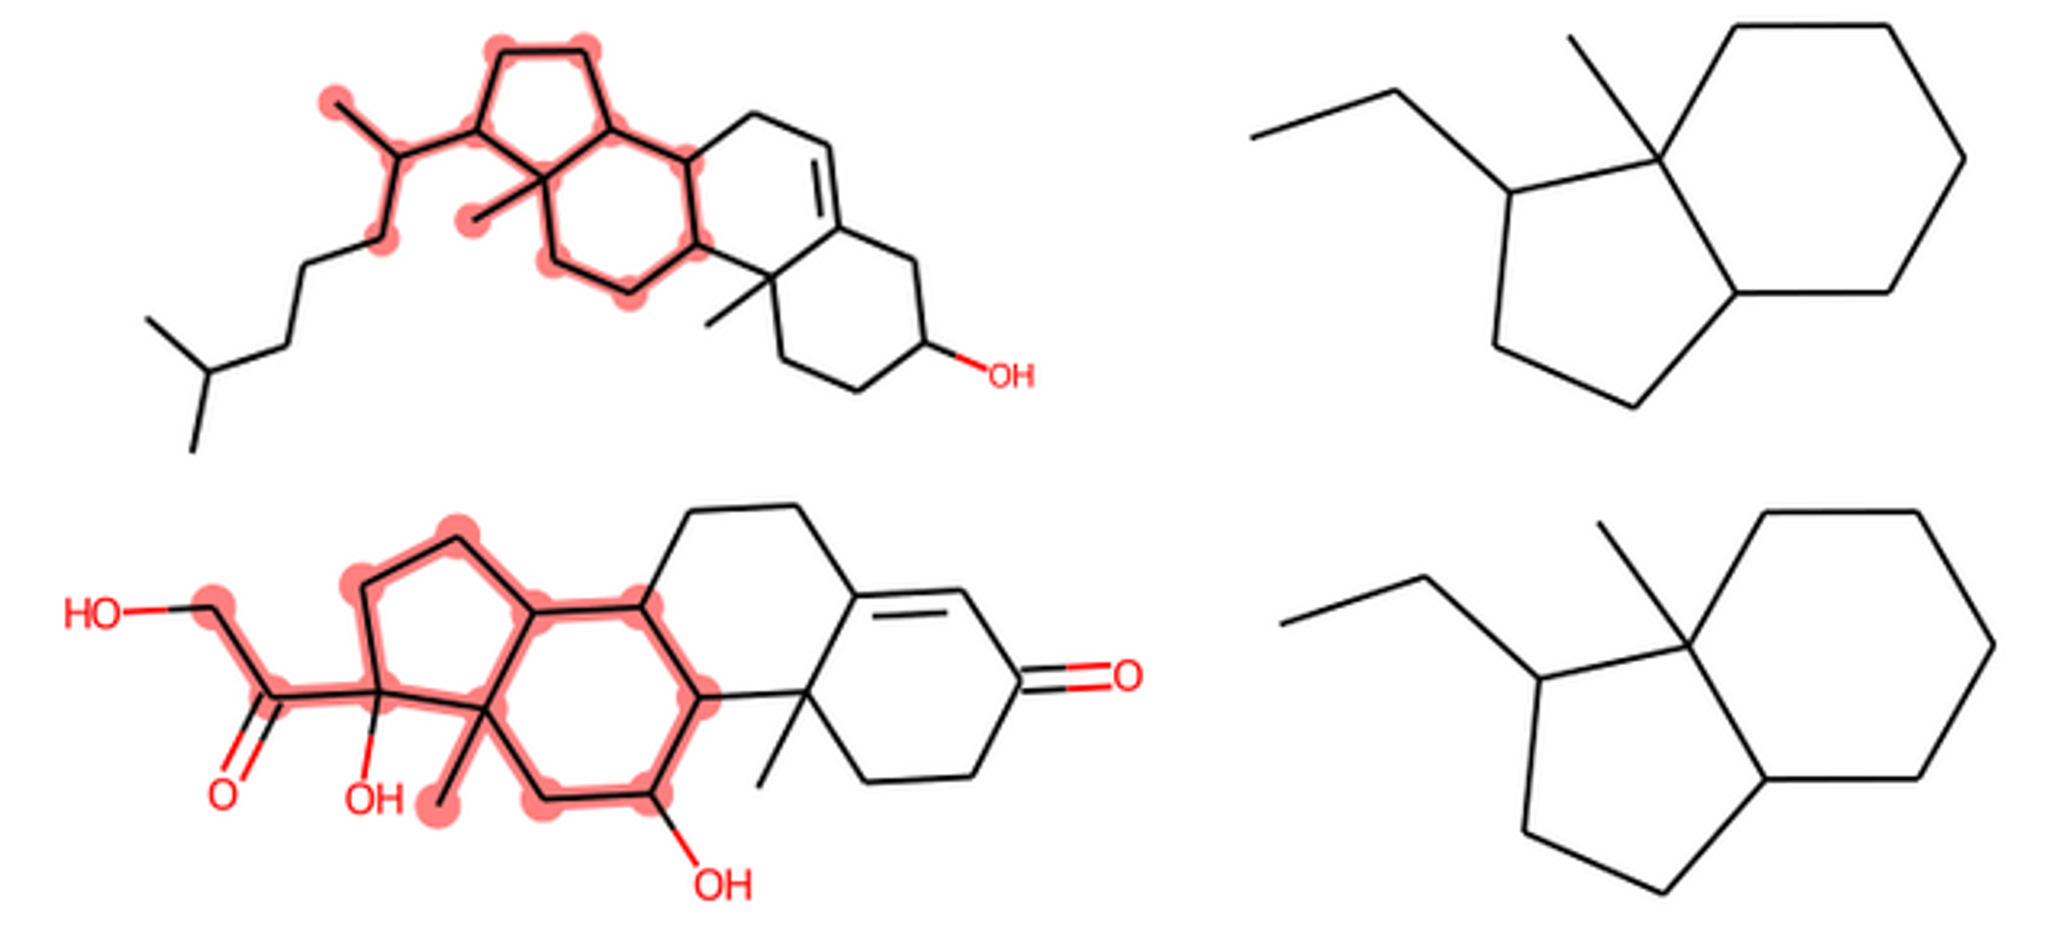
\includegraphics[scale=0.4]{sterols_w_strictfusion}

\caption{'Strict fusion' can affect the construction of the common core drastically, illustrated for cholesterol (top row) and cortisol (bottom row). First and second columns: common core of the two molecules without strict fusion; third and fourth column: common
core of the two molecules with strict fusion. In the images of the full molecule graph (first and third column), common cores are marked in red. In the example shown, none of the settings yield a valid common core for \trafo; the iterative approach explained in the main text would be necessary to obtain one. }

\end{figure}




\begin{figure}
	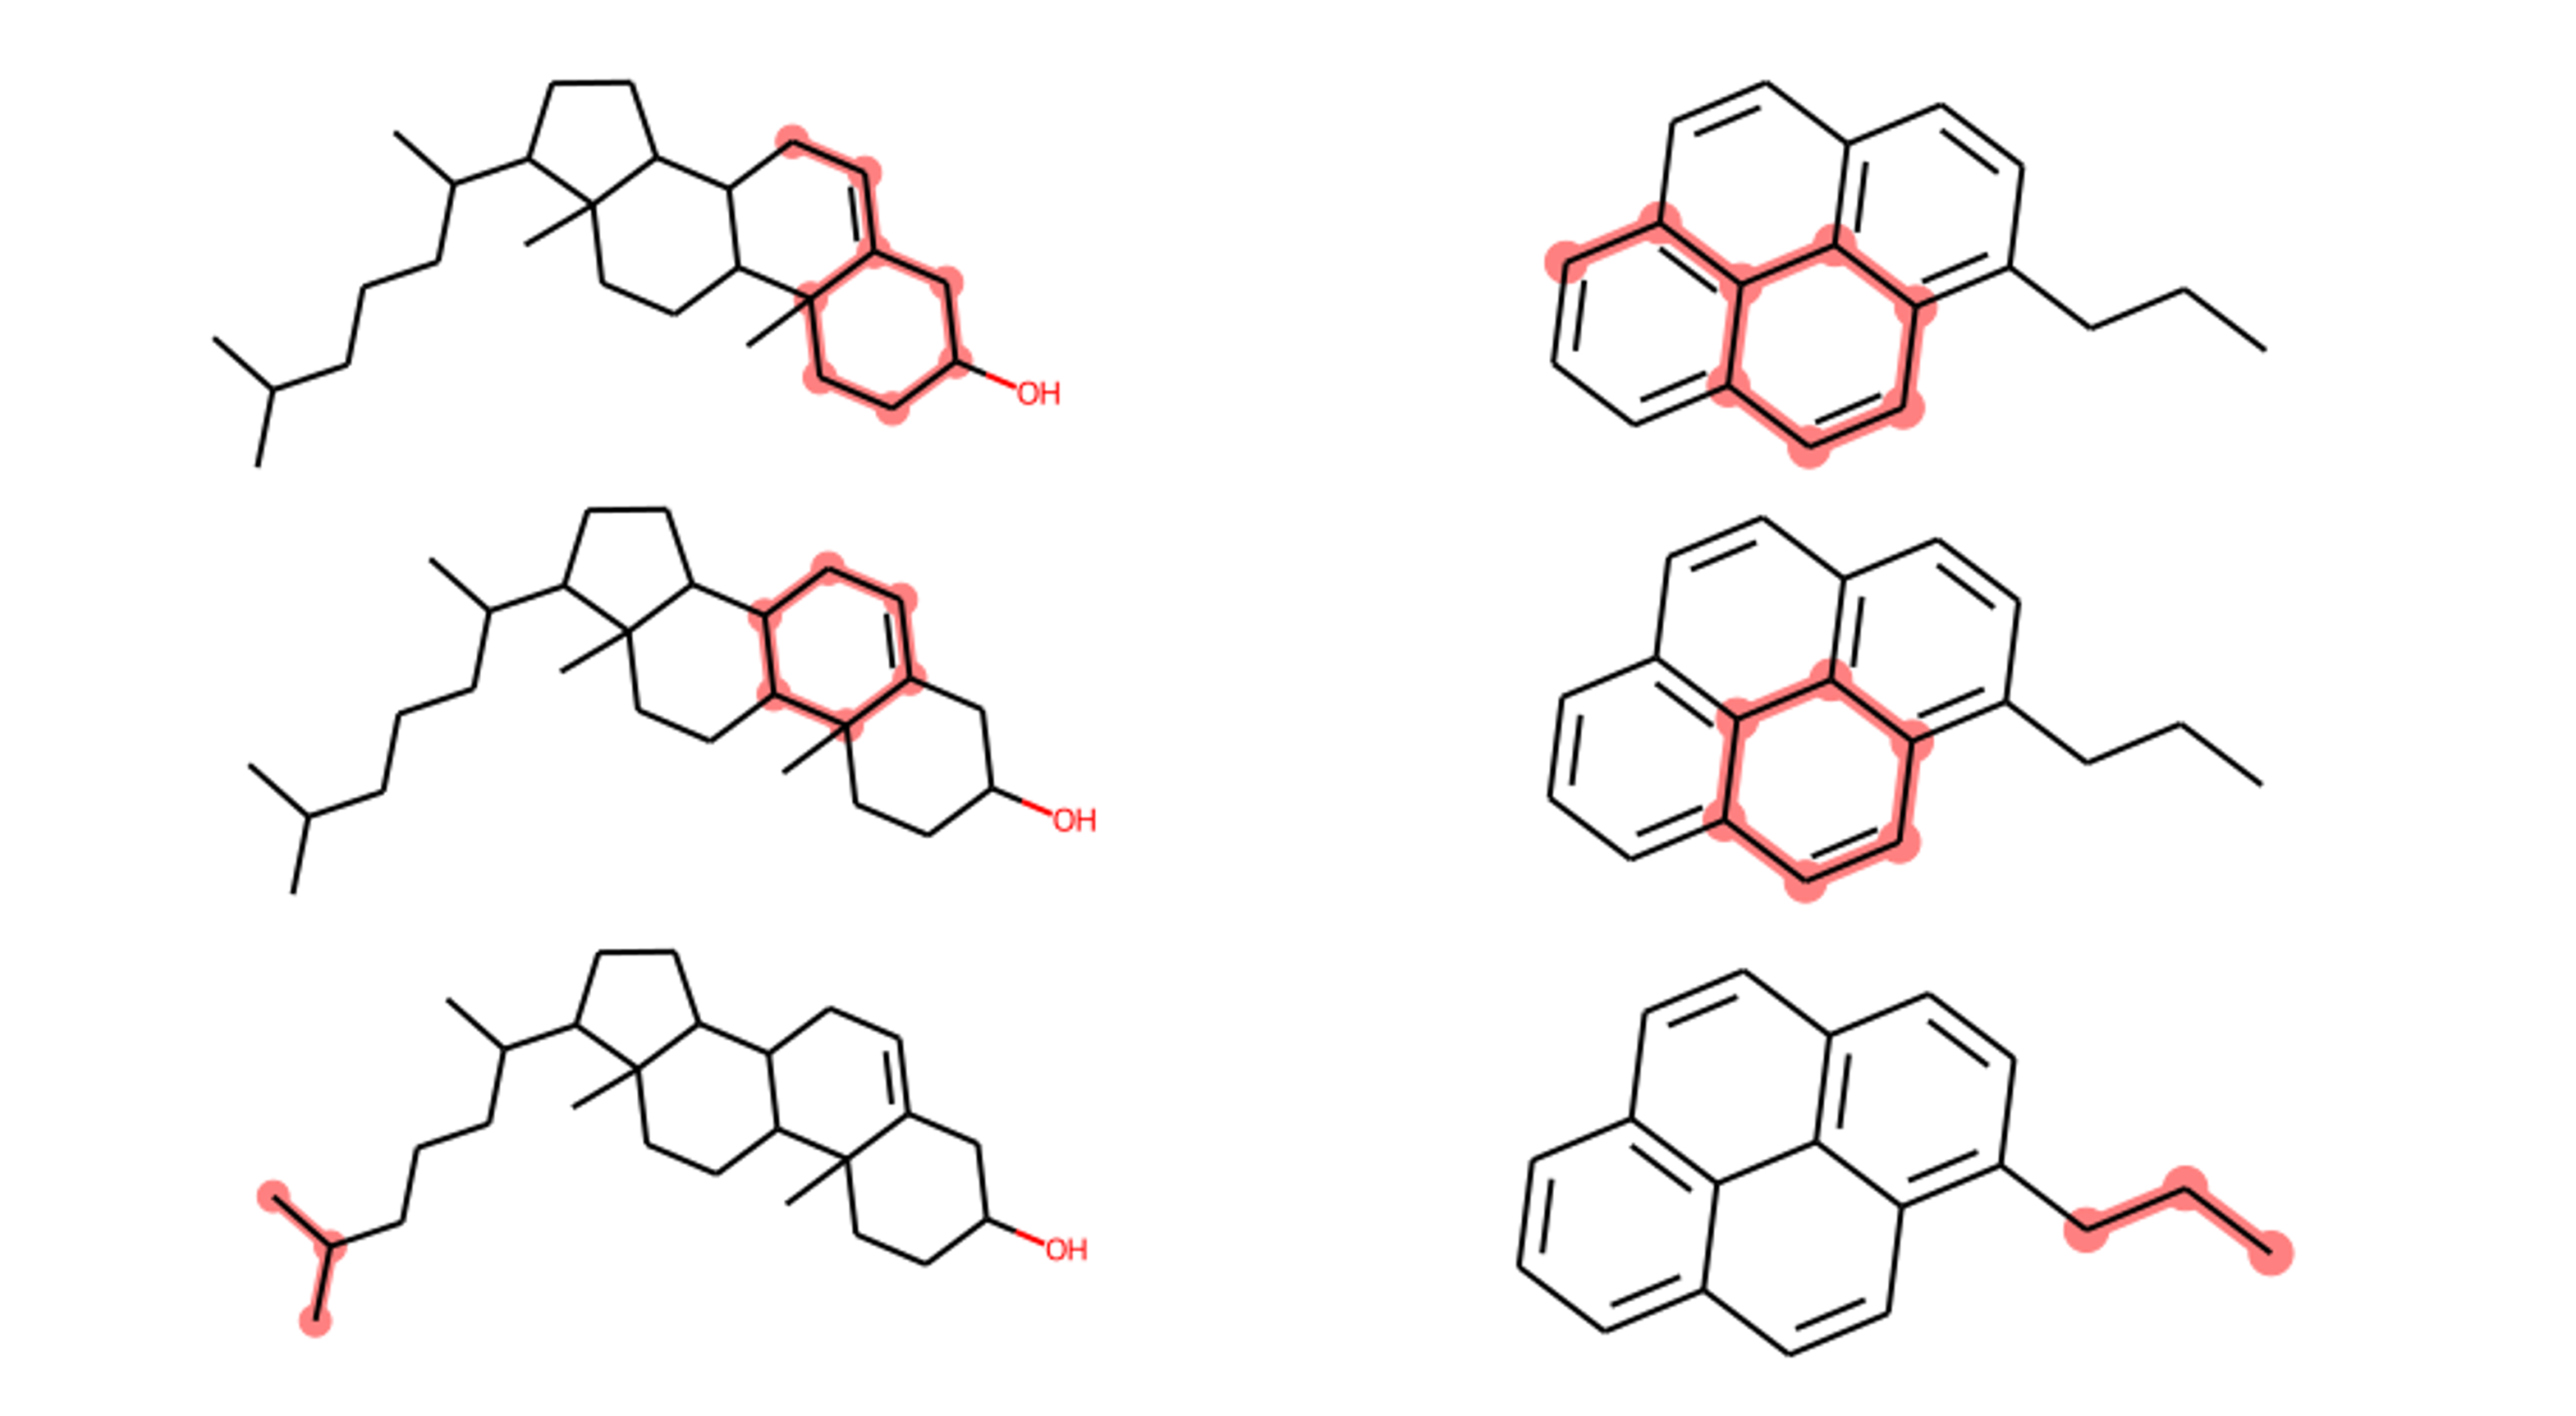
\includegraphics[scale=0.6]{cholesterol_pryenepropanoic_acid.png}
	
	\caption{Common cores of cholesterol (left) and 1-pyrenepropanoic acid (right); top row: CompleteRingsOnly = False; middle row: CompleteRingsOnly = True; bottom row: iterative approach to obtain a valid {\trafo} common core}
	\label{fig:pyrene}
\end{figure}

If this is not the case, the rings that contain atoms which participate in the partial ring causing the invalid common core are removed from the representation used for creating the maximum common substructure and afterward a new search for a valid common core is started. This procedure is repeated iteratively until a valid common core is found.
Of course, in the worst scenario, i.e., if both (non-identical) molecules only consist of ring-participating atoms, no valid common core is conceivable (and, given the total size of the molecules, the valid size can be tiny). In general, if at least one of the molecules solely consists of a polycyclic compound without any functional groups etc., and the other one does not have the same compound, no valid common core can exist. 
An --- maybe rather contrived --- example of such a pair of molecules and the construction of a valid common core via the iterative approach is given in Fig.~\ref{fig:pyrene}. One sees that even the usage of the ring-related parameters of Rdkit doesn't yield a valid common core, whereas the iterative approach gives the desired result.



\section{Graph algorithms}

Using NetworkX and Rdkit, the molecules and their common core are
represented as graphs (in which nodes indicate atoms and edges bonds
between them). The selection of the optimal mutation route can be
understood as a graph traversal problem, in which the constraints mentioned
above are either implemented via the weights of the edges or by sorting.
Hence, the main task was to find suitable algorithms and graph initializations
to ensure an optimal processing of the mutation path.

Depth First Search (DFS) follows each chain of the graph as long as
possible, i.e., until a leaf node is reached. In contrast, Breadth
First Search (BFS) explores all chains simultaneously.\cite{Even.2012}
Problems and differences of both algorithms are illustrated using
several examples below.

In each of the algorithms implemented, the root of the graph traversal is the node which connects the dummy region and the common core.
The shortest paths to all nodes of the dummy region are determined.

\begin{figure}

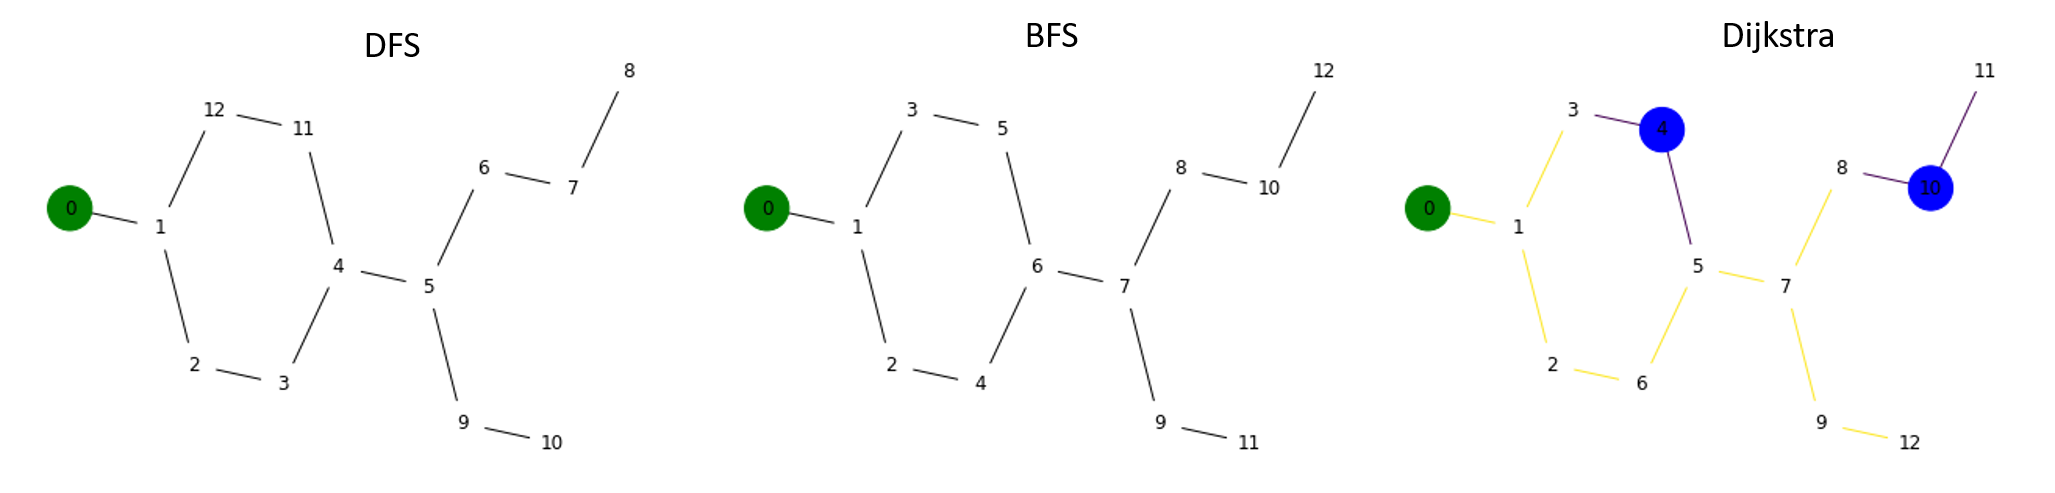
\includegraphics[scale=0.45]{dfs_bfs_dijkstra_comp1}\caption{Comparison of different graph traversal algorithms. Green nodes represent the root atom; left: depth first
search (DFS); middle: breadth first search (BFS); right: Dijkstra algorithm. In the Dijkstra algorithm, blue atoms have increased weights;  the
edges connecting blue colored nodes have increased weights leading
to a mutation route differing from BFS; the final processing of the
nodes happens in reversed order}

\end{figure}

The longest of these shortest path identifies the node which has the greatest
distance from the root (i.e., the atom with the greatest distance from
the common core). Therefore, the last element of the list returned by the search algorithm indicates the atom which has to be removed first; hence, the list of mutations orders has to be reversed.

If weighted graphs are used, the Dijkstra algorithm can be applied.
It finds the shortest path between two nodes or between a root node
and all other nodes of the weighted graph (the weights indicate the
edge length from one node to the other one). For unweighted graphs
(or, equivalently, graphs with uniform weights), the Dijkstra algorithm
reduces to BFS. Fig. 4.3 shows the different routes for modified weights.
In the test cases presented below, all graphs are initialized with uniform weights.

\section{New functionality added}

\subsection{Functions for creating mutation paths}

To use the newly implemented mutation algorithms, initially the graph
is given with weights stored in a dictionary. The simulations shown
below use uniform weights; however, it is possible to modify these to
enforce a specific mutation route (e.g., accelerating or postponing
the exclusion of heteroatoms). 

The Dijkstra algorithm is implemented via the \texttt{single\_source\_dijkstra}-function
of NetworkX.

\sbnote{Ich organisiere hier etwas um, weil mir der Text zu sehr "springt".}
The core functionality is given by the mutation processing functions.
Currently, three new functions are implemented, in addition to
the simple, existing DFS-approach.
These four main functions for computing mutation routes are: \sbnote{Why not use a list environment?}

\texttt{\_calculate\_order\_of\_LJ\_mutations:} naive DFS 

\texttt{\_calculate\_order\_of\_LJ\_mutations\_new:} BFS/Dijkstra-algorithm
applied once for route

\texttt{\_calculate\_order\_of\_LJ\_mutations\_new\_iter:} BFS/Dijkstra-algorithm
applied iteratively, i.e., after each removal of an atom 

\texttt{\_calculate\_order\_of\_LJ\_mutations\_new\_iter\_change:}
works iteratively; i.e., after each removal of an atom, the algorithm/routine for the next step is chosen depending on the current state

These functions
can be further modified by passing arguments which activate some helper
functions (see below).

\sbnote{, which leads to undesired outcomes, in particular because often heavy atoms in neighborhood to the common core atoms are processed at the first steps of the graph algorithm as well as rings are opened early, but completely processed at a later stage (in a rather 'asymmetric' manner).{\em Stoert die Praesentation und gehoerte mit Fig. 4.4 gemeinsam diskutiert. Entweder muss das schon vorher als Problem kommen, oder die Details muessen hier weggelassen werden, und auf die Result verweisen!!}}

\texttt{\_calculate\_order\_of\_LJ\_mutations } is the original mutation processing function of \trafo, but it may lead to  defective mutation routes and hence
should only be used for test purposes. The other three algorithms
are new, and all of them resolve most of the problems of the earlier
algorithm (especially isolated removal of ring atoms).

Helper functions like cycle\_checks carry out tasks to ensure the
desired mutation route, e.g., count the number of cycles an atom participates
in. Further features of all algorithms are 'preferential removal';
i.e., if two atoms have the same priority (given by the current
weight) for the next mutation step, the weight of the atom which is
next to an already removed atom is updated so that this atom is excluded
next.

\sbnote{What is (G)? Ich nehme an ein Graph(objekt) Argument. 1) Definieren! 2) Generell klarer machen, dass hier Funktionen und ihre Argumente beschrieben werden, auch auf Typesetting achten!}
\texttt{cycle\_checks(G)}: this function checks which atoms participate
in how many cycles/rings and returns a dictionary with the atoms as
key and the number of rings the atom is participating in as value
and a dictionary with the degree (i.e., number of edges) of each atom
node. It is currently used in \texttt{\_calculate\_order\_of\_LJ\_mutations\_new}
(via the \texttt{change\_route\_cycles}-function).

\texttt{change\_route\_cycles}(route, cycledict, degreedict, weightdict,
G): this function is used in \texttt{\_calculate\_order\_of\_LJ\_mutations\_new}
and sorts nodes according to degree, cycle participation and information
about the nodes which have been removed immediately before. The preliminary mutation
path is sorted using a cycle and degree dictionary. If nodes have the same
weight (i.e., distance from root), the node participating in more cycles
is removed later. If nodes have the same weight (i.e., distance from root)
and same cycle participation number, the node which has more neighbors
already removed is removed earlier

\texttt{cycle\_checks\_nx}(G): This function modifies the weight of
the graph, nodes participating in many cycles get lower weight. It
is currently used in 
\texttt{\_calculate\_order\_of\_LJ\_mutations\_new\_iter} and \texttt{...\_new\_iter\_change.} It returns a nx-graph-object
with updated weights (according to cycle participation of the atom).

\texttt{order\_checks\_nx}(G, removearray, G\_total): This function
performs the 'preferential removal', if a node is connected to the
node removed in the last step, its weight get a small increase so
that the removal of this node is prioritized. It is currently used
in\texttt{ \_calculate\_order\_of\_LJ\_mutations\_new\_iter} and returns
a nx-graph-object with updated weights.

If the cyclecheck-argument of the new mutation algorithms is True,
updates are updated according to cycle participation (as the systematic
processing of ring structures is one of the central goals, this argument
should always be set to True, except for comparison and test purposes).
If in the case of \texttt{\_calculate\_order\_of\_LJ\_mutations\_new
and \_calculate\_order\_of\_LJ\_mutations\_new\_iter} also ordercycles
or ordercheck, respectively, are set to True, weight updating according
to preferential removal decides that the node in which neighborhood
nodes have already been turned off is removed next if there is no
possibility to decide between two nodes --- i.e., the weight of both
would be the same.

In each algorithm, all nodes of the graph (i.e., atoms) are usually
initialized with the same weight (e.g., 5). Alternatively, the user
could also pass an individual dictionary with different weights for
each atom type.

The BFS- / Dijkstra-algorithm starting from the node connecting common
core and dummy region is applied via the NetworkX-function \texttt{single\_source\_dijkstra}
which determines the path length of all dummy nodes to the root.

The main difference between these algorithms is that in \texttt{\_calculate\_order\_of\_LJ\_mutations\_new\_iter}
and \texttt{...\_iter\_change} the graph traversal part performed
using the Dijkstra algorithm is applied after each exclusion step; i.e., $n!$ atoms are visited instead of $n$; even for large molecules the additional computational cost is negligible, in particular in comparison
to the computational time needed for the search of the common core.
The advantage of the iterated version is that after each mutation step, weights can be
updated or even the search algorithm can be modified. 

This feature allows for different mutation strategies depending
on the current state. Such an approach is demonstrated in \texttt{\_calculate\_order\_of\_LJ\_mutations\_new\_iter\_change}.
In contrast to the other algorithms, the algorithm processes information
if the last removed node was part of a chain or a cycle. Depending
on the state, the chain, or cycle, is processed fully before the algorithm
moves on to other parts of the molecule. \sbnote{1. Keine absoluten Verweise auf Figuren! 2. Fig. 4.4 wurde noch nirgends besprochen!} Fig. 4.5 demonstrates the difference between the two versions of the iterated algorithm.
Whereas in the non-iterated algorithm the found mutation route has to be reversed (since the atom node with the highest distance from the root is the first which has to be turned off), in the iterated versions at each iteration the node with the highest distance is added to an array which determines the final mutation route.

The computed mutation routes can be visualized directly via Rdkit. 
The route is represented by a color gradient used for the atoms involved
in the mutation process (\texttt{\_show\_common\_core\_gradient}). By default, the color spectrum ranges from red to green; the first atom to be removed is colored red, the last green.

Furthermore, an animated 3D-visualization of the mutation process
is implemented using py3Dmol (\texttt{animated\_visualization\_3d\_v2})\cite{key-4}. 

\begin{figure}
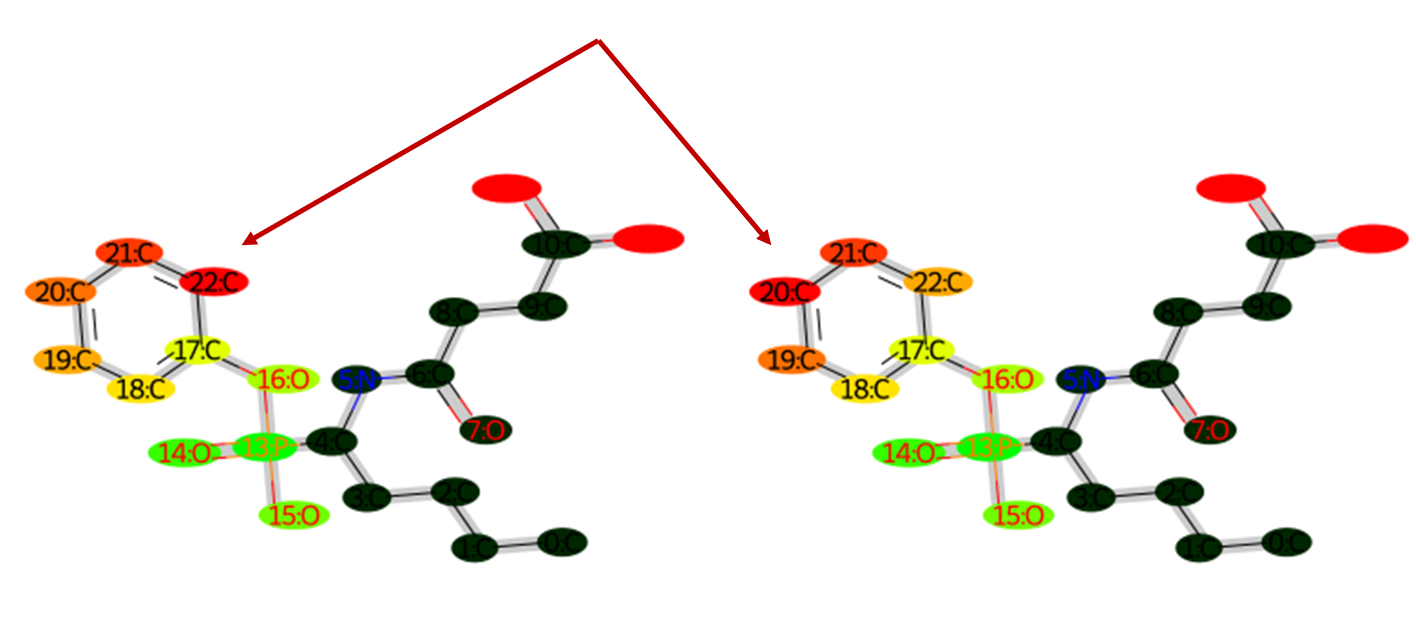
\includegraphics[scale=1.4]{simple_ring_exampledfs.png}

\caption{comparison of typical DFS- and BFS-mutation route for a single ring structure; left: DFS-algorithm; right: BFS-algorithm; in all depictions of mutation routes the common core is shown in dark, the color gradient starts at red indicating the atom first to be removed and ends at green; DFS
starts at carbon 22 and thus ring breakage gives rise to one long
chain which is processed subsequently, whereas BFS starts at carbon
22 and the two emerging chains are processed in a symmetric fashion \sbnote{Figur ist entweder falsch positioniert oder gehoert frueher besprochen, referenziert}
}

\end{figure}


\subsection{Processing of hydrogen atoms}

\begin{figure}
	
	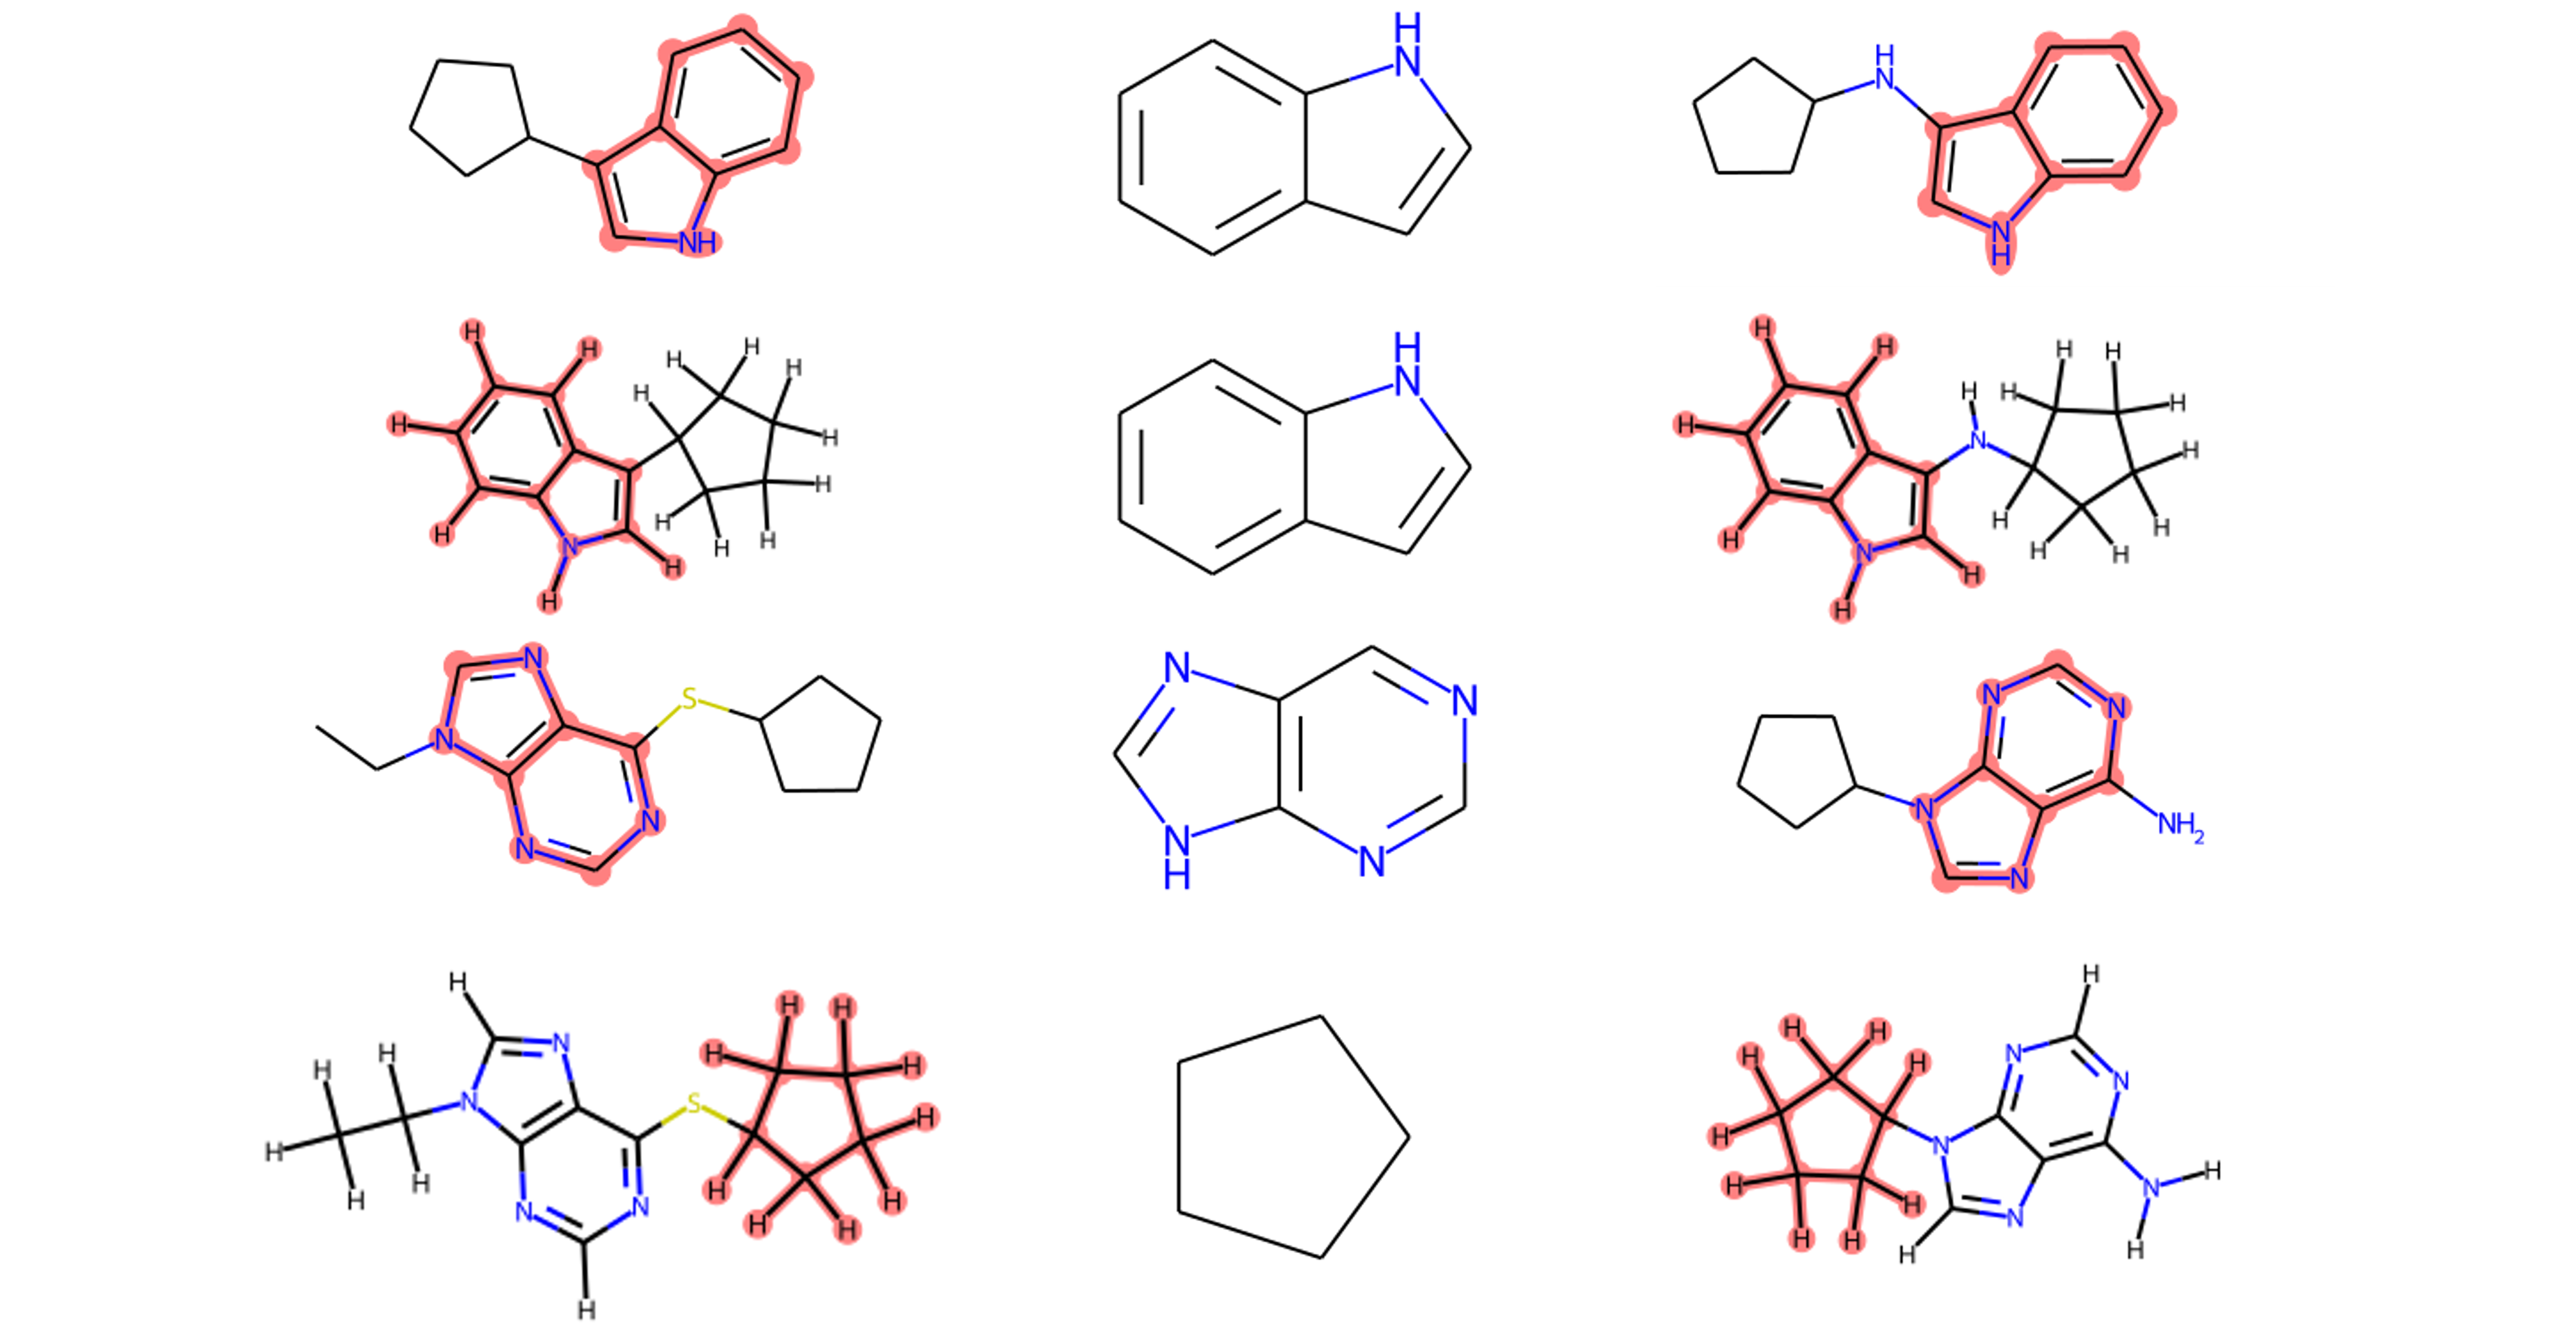
\includegraphics[scale=0.35]{hydrogens_plus_minus}
	\caption{These examples demonstrate that the addition of hydrogens can influence the construction of the common core; left: molecule 1; middle: common core; right: molecule 2; in the representations of the full molecule, the common cores are marked in red; the first
		and the last two rows show the same molecules, in the upper row without,
		in the lower with hydrogens, in case of the lower molecule combination
		the common core changes when hydrogens are added to the Rdkit-molecule
		representation \sbnote{Eine Nummerierung der horizontalen Reihen von 1--4 waere hilfreich. Die gelbliche(?) Farbe in Reihen 3 + 4 ist kaum sichtbar.}}
		\label{fig:hydrogen_effect}
	\end{figure}


As fig. \ref{fig:hydrogen_effect} indicates, the presence of hydrogens can influence the common core generation dramatically. In particular, the maximum common substructure for a molecule representation with hydrogens can encompass less heavy, i.e., non-hydrogen, atoms than the substructure for a representation with hydrogens removed (although, including the hydrogens, the total number of atoms is higher in the first case). Hence, it is crucial to determine the common core for molecule representations without hydrogens. Since hydrogen atoms are turned off in an extra step en bloc during the {\trafo} workflow, the mutation route algorithm should not take hydrogens into account, nor must the common core be generated for a molecule representation containing hydrogens.
Nonetheless, it is necessary that the molecule representations processed by \trafo contain all hydrogens in explicit form because the indices of these atoms in the underlying data structures are used in some steps, e.g., for scaling the van der Waals interactions of the hydrogen atoms to zero.
This problem was solved by removing and adding hydrogens appropriately.
In a first step, the {\trafo} function determining the common core (\texttt{\_find\_mcs} in mutate.py) had to be modified. To obtain the desired common core but retain the {\trafo} workflow, the following scheme was implemented:
A deep copy of both molecules is created. The hydrogens of these copies are removed; then their common core is computed. For both molecules, the indices of the atoms corresponding to the common core are determined. Finally, it is checked for each common core atom of both molecules whether hydrogen atoms are in its neighborhood. If such hydrogens are found, their indices are added to the lists of common core atoms. These lists of atoms, including hydrogens, are stored for both molecules and the function returns the maximum common substructure (determined for the molecules without hydrogens).
Thus, the procedure yields the necessary output for further processing in {\trafo}: The molecule representations and lists of common core atoms for both of the molecules include hydrogens, but the maximum common substructure giving rise to the common core is computed only for the heavy atoms.
Similarly, the functions for computing the mutation routes had to be adapted for input molecules containing hydrogens. By default, a helper function removes the hydrogens from the graph representation as well as the corresponding indices from the list with the atoms of the dummy regions before the mutation algorithms are applied. Afterward, the hydrogen atoms adjacent to common core heavy atoms are added to the common core.
A special problem occurs for molecule pairs with switching 'X'-atom; fig. \ref{fig:pyrrolidinindole} shows 2-/7-pyrrolidinindole as an example. It is necessary that a further dummy region emerges which consists solely of one hydrogen atom because otherwise the common cores would have a different number of atoms. It depicts a correct common core for both molecules; one should note the hydrogen atom, which is not part of the common core. If, however, the common core is generated without hydrogens, the information which of the hydrogens turns into a dummy region is lost.
It has to be stressed again that the presence of these hydrogen dummy regions does not affect the mutation steps, but is nonetheless crucial for the internal {\trafo} workflow. However, there is a straightforward way to circumvent this problem: From the substructure matches, the mapping between the common core atoms of each molecule can be read off. It is counted for each heavy common core atom how many hydrogens are connected to it. Finally, the minimum number of hydrogens is added to the common core. (In the case of 2-/7-pyrrolidinindole, this means that for each common core atom one hydrogen is added, except for the 2- and 7- position because for these positions in one molecule no hydrogen is connected).
In this context, also the difficulty that there are possibly many substructure matches has to be mentioned.
It is even possible that substructure matches differ solely regarding hydrogens. For this case, a parameter was added to the function which searches for the maximum common substructure. If \texttt{iterate\_over\_matches} is set to true, one of the substructure matches with most hydrogens, i.e., the biggest possible substructure, is selected. Fig. \ref{fig:neopentan} shows two common cores, only differing in the number of hydrogens.



\begin{figure}
	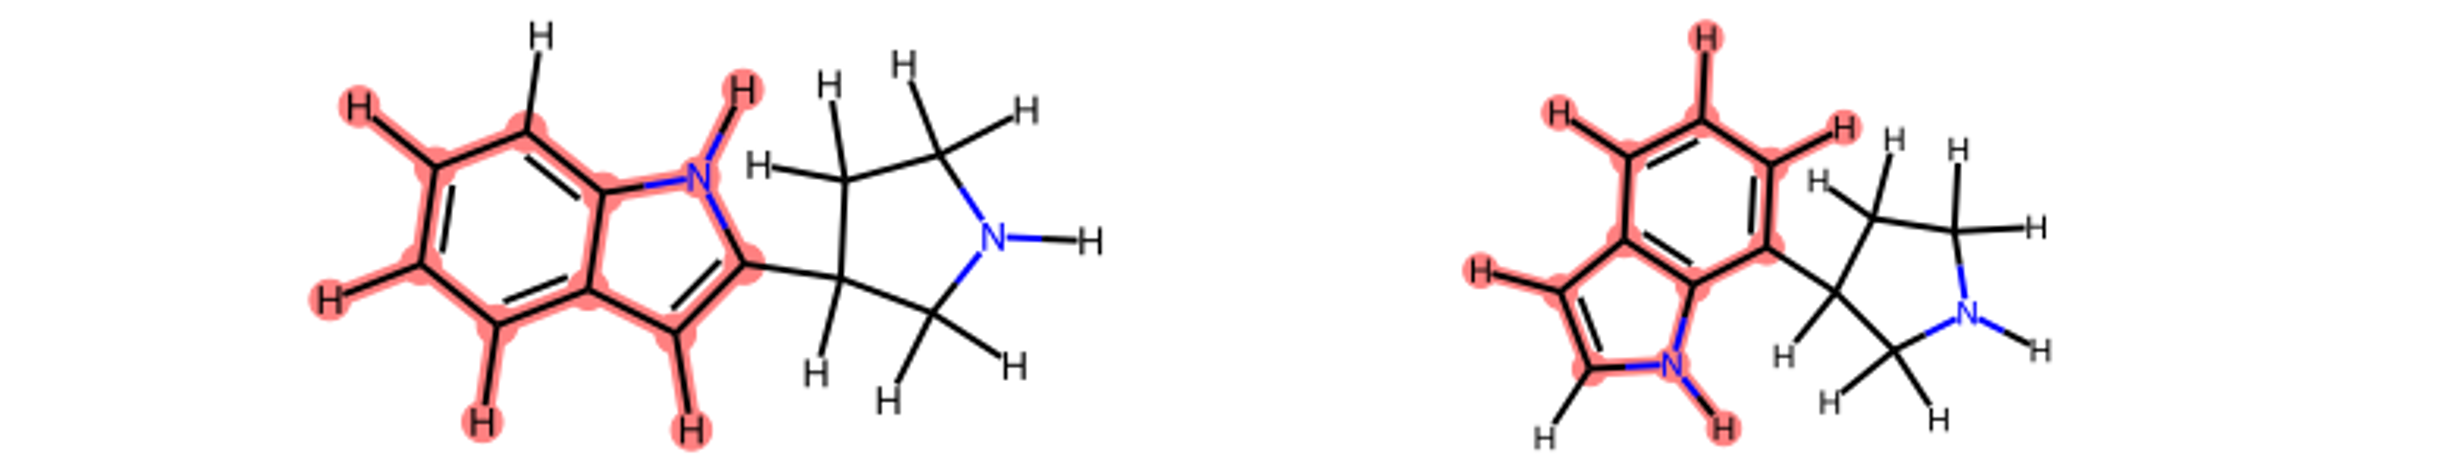
\includegraphics[scale=0.8]{pyrrolidinindole}
	
	\caption{
		left: 2-pyrrolidinindole; right: 7-pyrrolidinindole; 
		one of the hydrogens --- exactly this hydrogen which becomes the junction 'X'-atom --- is not part of the common core}
	\label{fig:pyrrolidinindole}
\end{figure}


\begin{figure}
	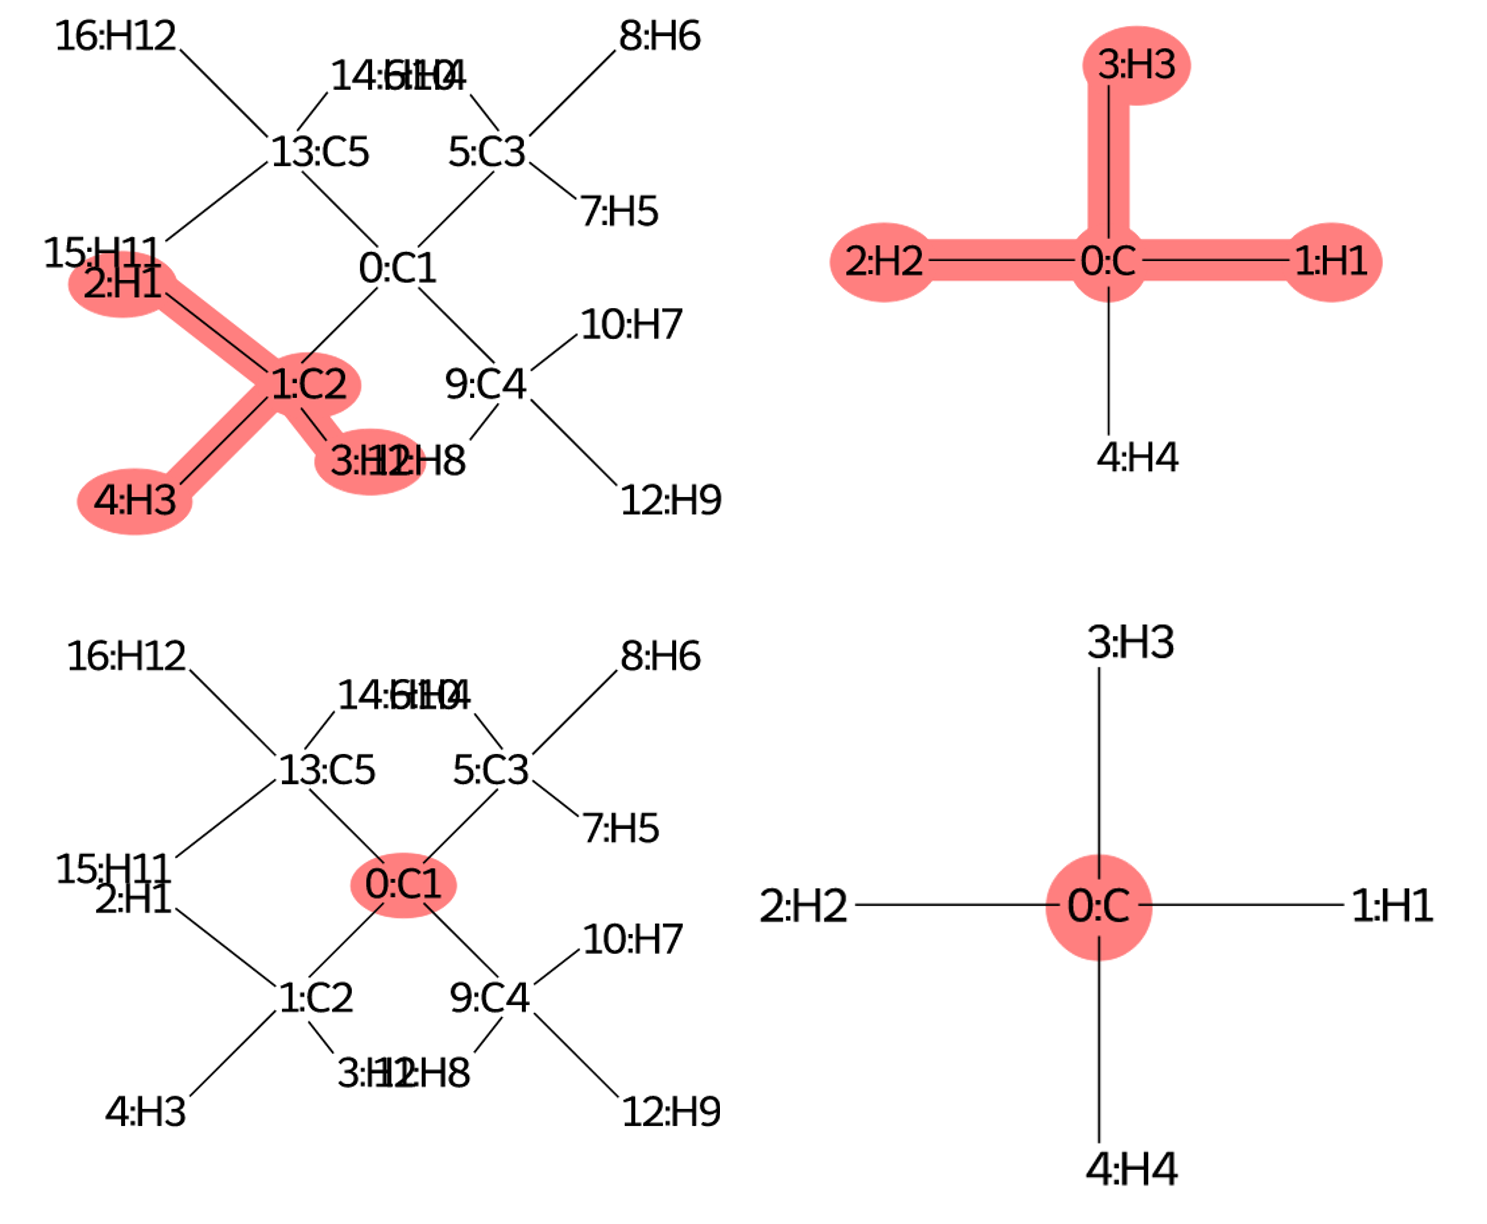
\includegraphics[scale=1.0]{neopentan}
	
	\caption{neopentane/methane common cores; upper row: common cores maximizing the number of atoms including hydrogens; lower row: common cores without considering hydrogens \sbnote{In der Figur ueberlappen die Atombezeichnungen.}}
		\label{fig:neopentan}
\end{figure}



\subsection{Examples for processing molecules}

\begin{figure}
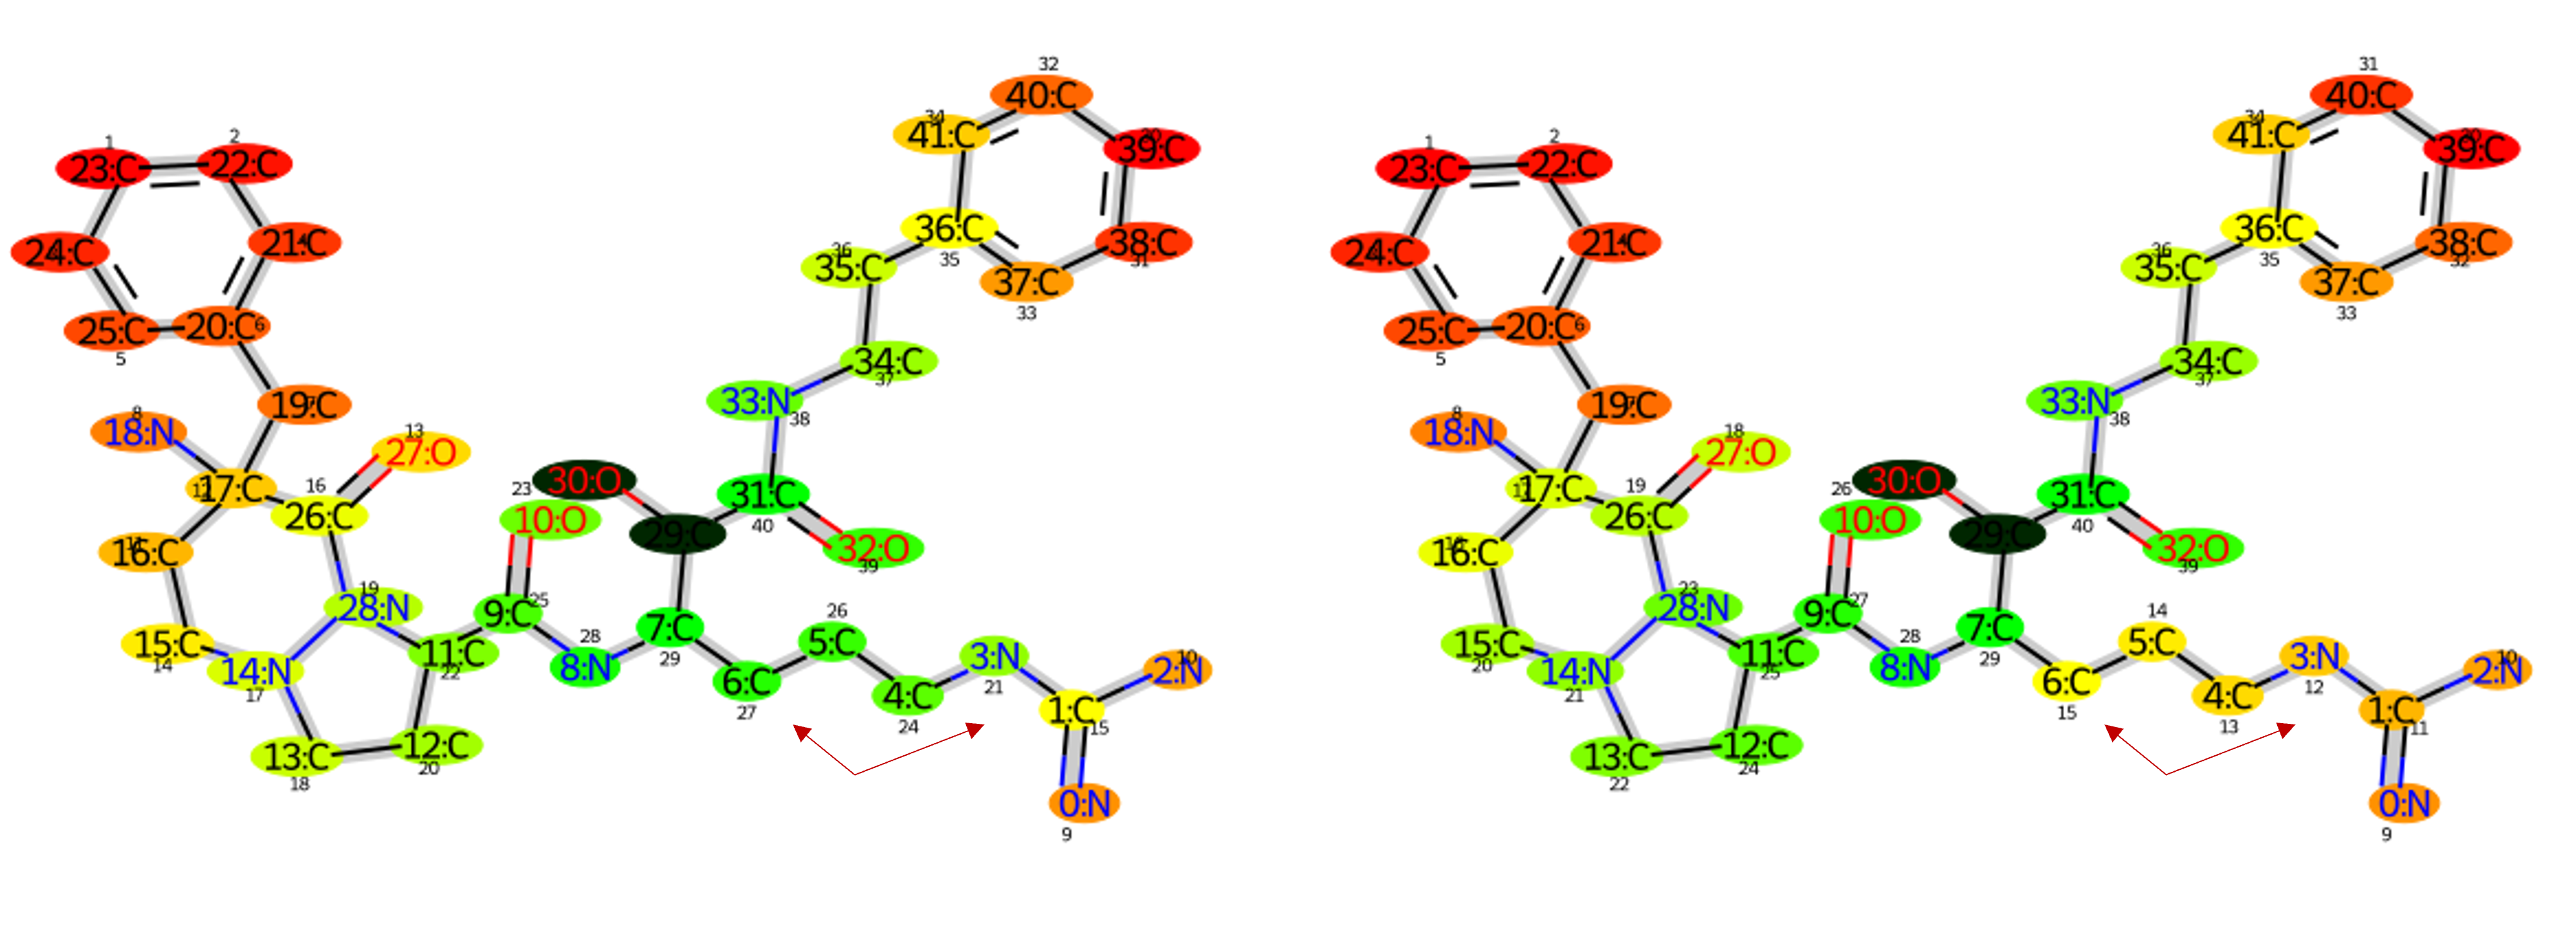
\includegraphics[scale=0.5]{iter_iter_change_1a5g_1}

\caption{Example for the differences between iter- and iter\_change-algorithm;
left: iter; right: iter-change; iter-change processes all atoms within
a chain or a ring at once (if possible) before switching to other
parts of the molecule}
\end{figure}

In the current version of {\trafo}, one suboptimal route finding algorithm using DFS and several new versions based on BFS are implemented.
For single rings, BFS (or, in the case of different weights for various atom types, the Dijkstra algorithm) automatically processes the atoms in the most symmetric way starting at the atom with the highest distance from the root (fig 4.4).
In more complex molecules, the systematic exploration of chains in
depth first search inevitably leads to big local gaps in processing
of the molecules. Fig.~4.6 shows this problem for a benzene ring which
is directly attached to the common core. As DFS goes along one path
until the end; i.e., until a leaf node is reached, four atoms of the
ring are visited first, whereas the remaining two are explored
last. Therefore, these two atoms are turned off first, but then the
algorithm continues at a wholly different location and the remaining
ring atoms persist in the system until the end of the mutation process.
By contrast, BFS automatically produces the desired result for this system. 

Similarly, in fig. 4.7 one atom of the ring (marked by the red circle)
is omitted in the first exploration using DFS.

More complex ring structures exacerbate the problems. Fig. 4.8 shows that also the processing of the substituents is affected.

Multiple rings pose special difficulties for the mutation algorithms because
the processing of one of the rings can easily lead to gaps in the adjacent
ones. Fig. 4.9 and 4.10 illustrate that severe problems may occur when using DFS.
As in the case of one ring, the exploration route implies that one
of the rings is opened in such a way that it gives rise to a lengthy chain.
Furthermore, it may happen that the atom explored atom belongs to two or more rings, so that both ring structures are opened
and teared apart (fig. 4.9). Alternatively, one half of each of the
rings is turned off first (fig. 4.10). 

\begin{figure}
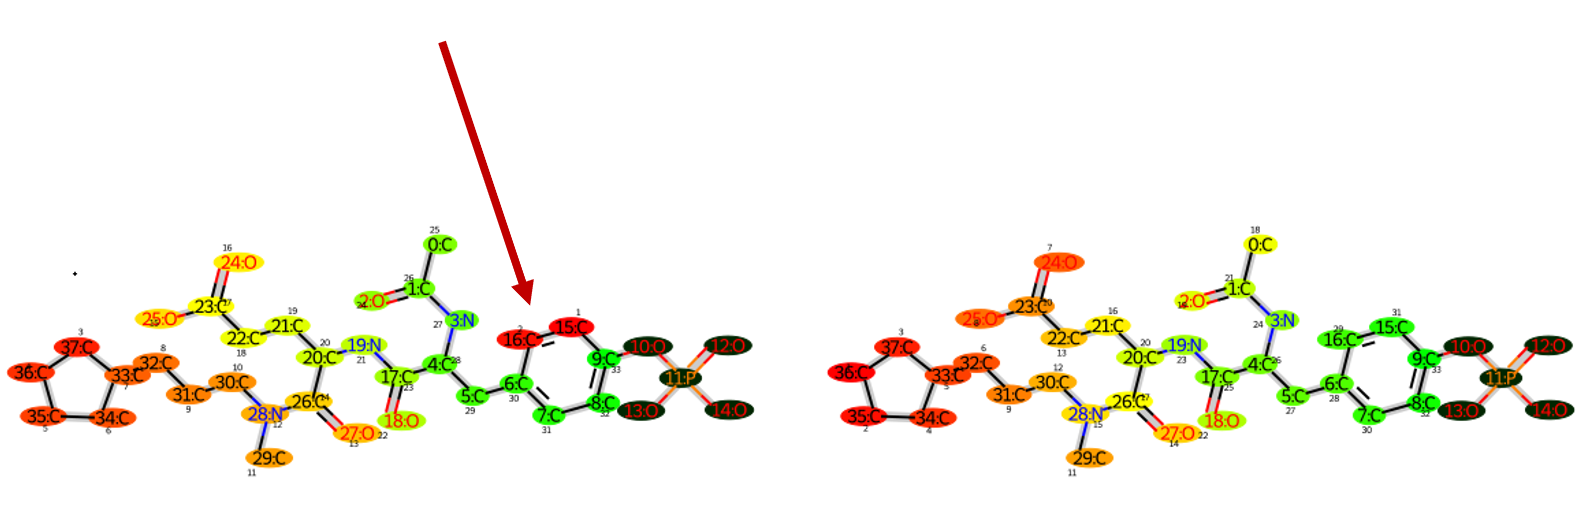
\includegraphics[scale=1.5]{simple_ring_exampledfs2}\caption{left: DFS-algorithm; right: BFS-algorithm; common core in dark; the
red arrow indicates the undesired processing of the ring atoms \sbnote{Die rechte Figure ist abgeschnitten, CC nicht sichtbar!}}

\end{figure}

\begin{figure}
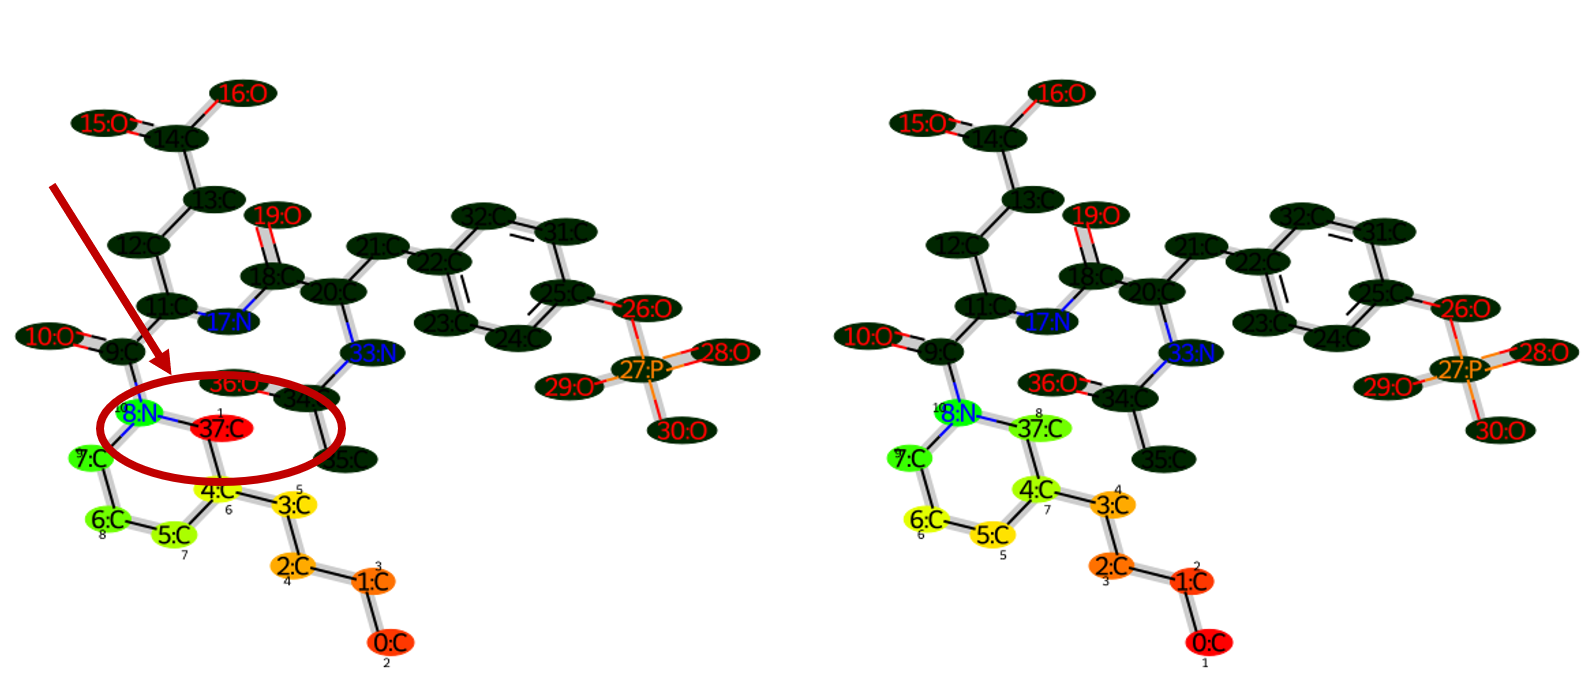
\includegraphics[scale=1.3]{simple_ring_exampledfs3}\caption{left: DFS-algorithm; right: BFS-algorithm; common core in dark; the
red arrow and circle indicates the undesired processing of the ring
atoms}

\end{figure}
\begin{figure}

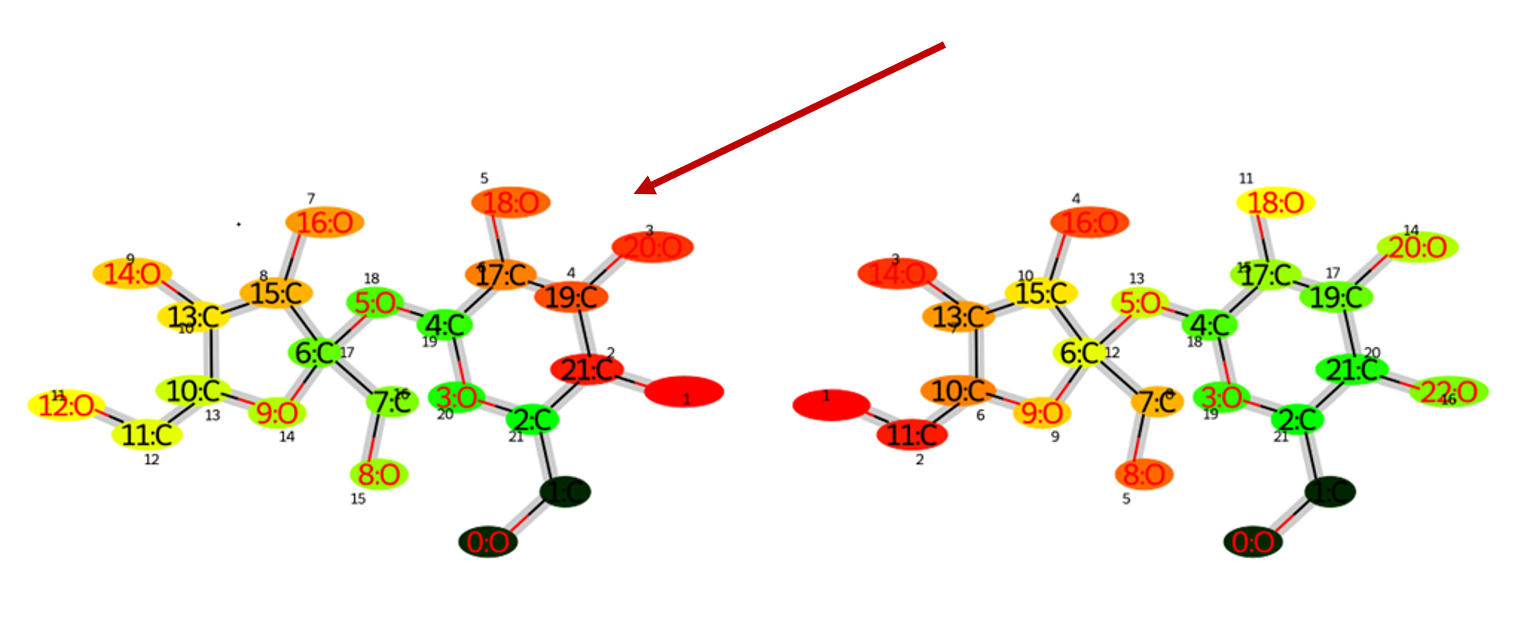
\includegraphics[scale=0.5]{simple_ring_exampledfs4}\caption{left: DFS-algorithm; right: BFS-algorithm; common core in dark; the
red arrow indicates the undesired processing of the ring atoms}

\end{figure}

\begin{figure}

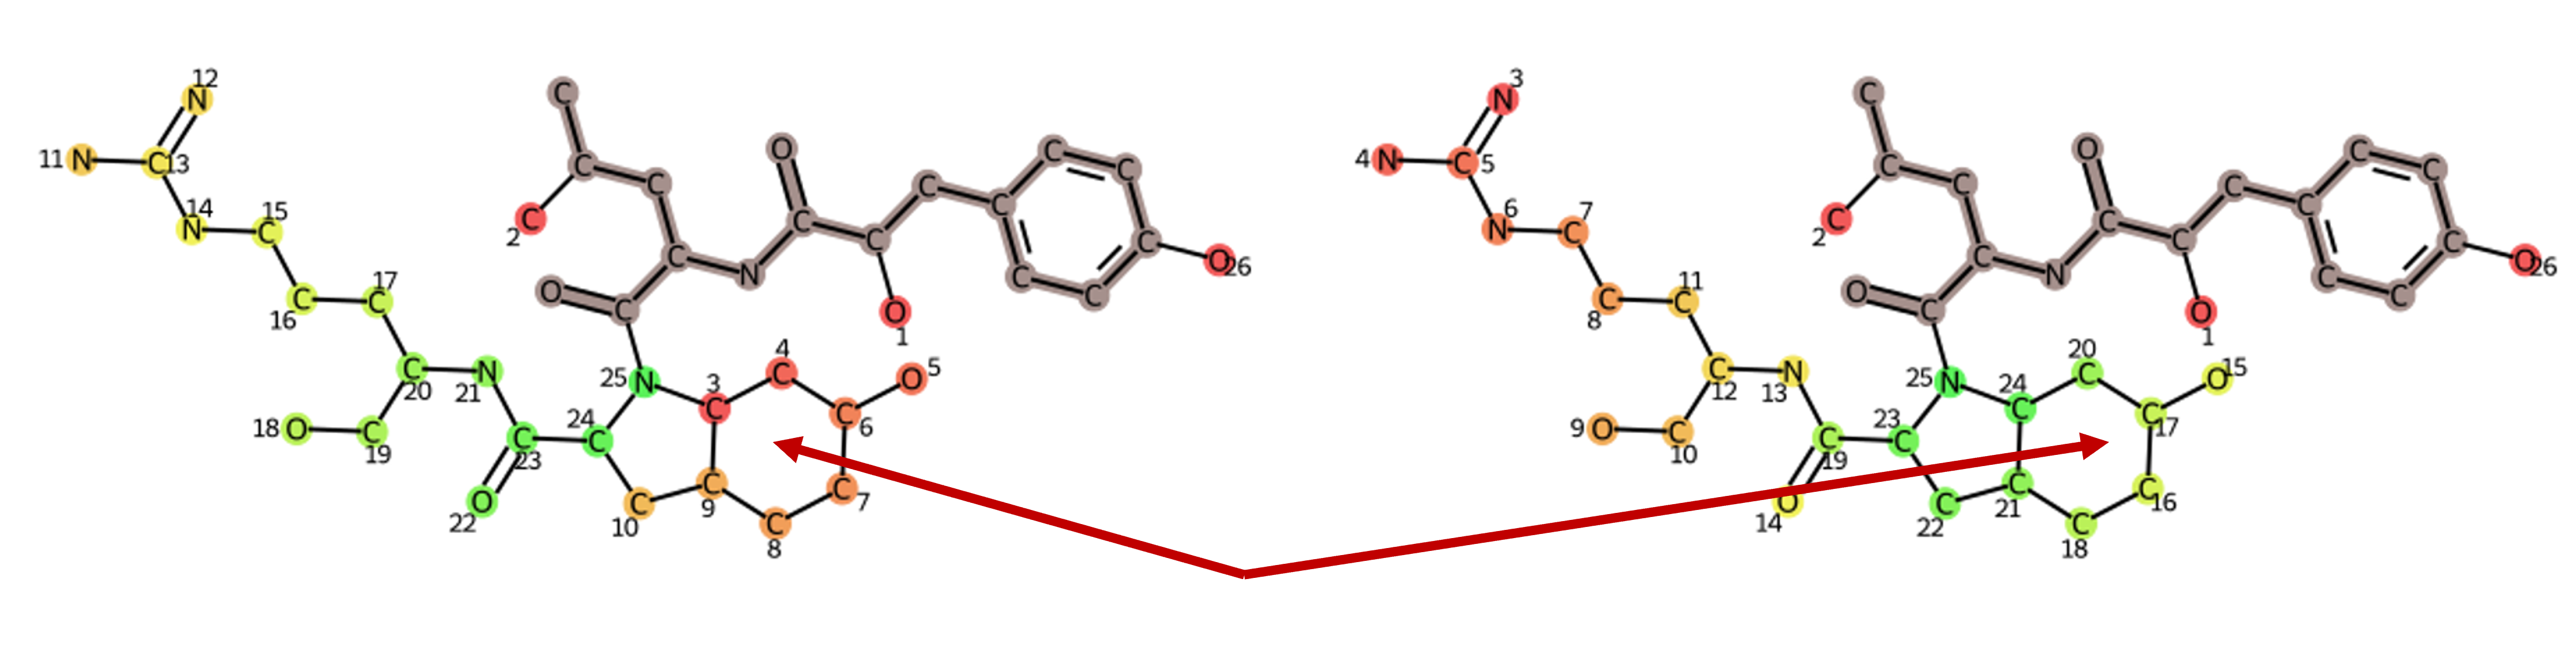
\includegraphics[scale=0.5]{2ring_example}\caption{left: DFS-algorithm; right: BFS-algorithm; common core in dark; the
red arrow indicates the undesired processing of the ring atoms}

\end{figure}

\begin{figure}

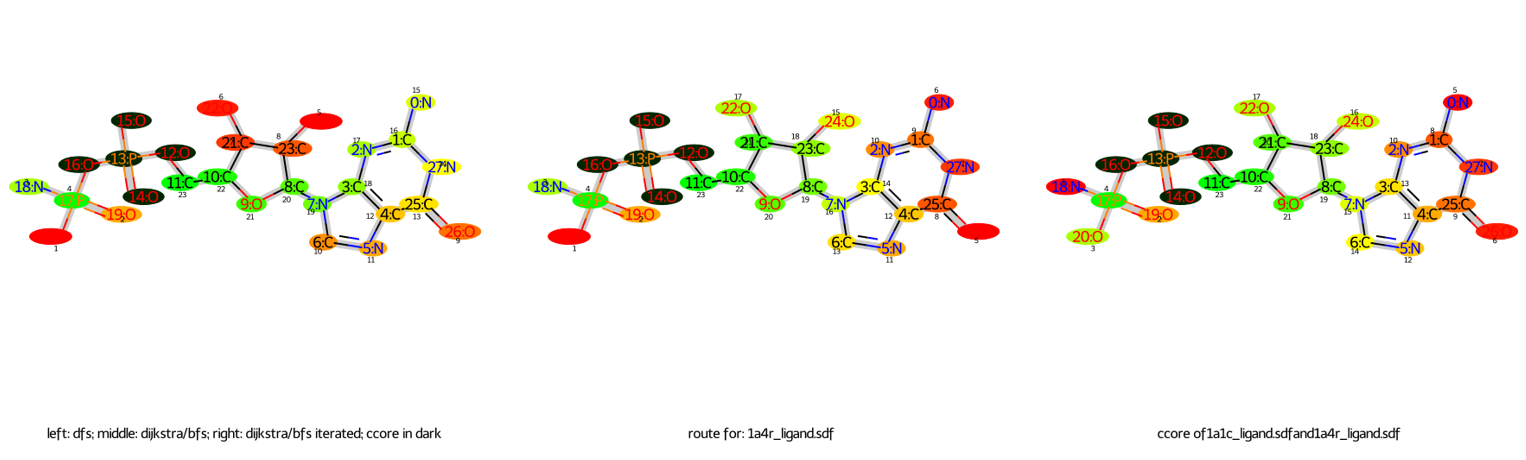
\includegraphics[scale=0.5]{2ring_example2}\caption{left: DFS-algorithm; right: BFS-algorithm; common core in dark}

\end{figure}

	\chapter{Results}

\begin{table}[!t]
	\begin{tabular}{|>{\centering}p{2.5cm}|>{\centering}p{2.5cm}|>{\centering}p{2.5cm}|>{\centering}p{2.5cm}|>{\centering}p{2.5cm}|}
		\hline 
		number of processed routes & dummy atoms (mean) & atoms/dummy region (mean) & number of cycles (mean) & polycyclic {[}\%{]}\tabularnewline
		\hline 
		378 & 26.97 & 16.30 & 1.66 & 30.16\tabularnewline
		\hline 
	
	\end{tabular}\caption{Some statistics about the twenty ligands selected from the PDBbind-CN database and the calculations they were used for. Number of processed routes: total number of computed routes for a specific combination of two molecules; dummy atoms (mean): average number of total dummy atoms required for the computed mutation routes; atoms/dummy region (mean): number of total dummy atoms divided by the number of dummy regions; number of cycles (mean): average number of cyclic structural elements in all mutation routes; polycyclic: percentage of mutation routes which involve polycyclic structures, i.e., there are atoms present that participate in multiple cyclic elements }
\label{tab:general_information}
\end{table}

A set of twenty ligands from the PDBbind-CN database were downloaded and used for testing
CC construction, as well as mutation routes. General information about the ligands can be found in table \ref{tab:general_information}. 
It should be noted, however, that the CCs for some of these ligand pairs
violate the rules of {\trafo} concerning a valid CC; i.e., dummy regions are connected by more
than one atom to the CC (which basically implies that the
atom is part of a ring structure). 

In the current implementation of the mutation algorithm, this problem
is solved by a helper function which chooses one of the possible connections
between one of the atoms to the CC. For the following processing
of the mutation algorithm, this connection is arbitrarily distinguished
and the other ones removed. 


\section{Visualizations}

The mutation route is visualized using a color gradient, in addition
to numbering, see the earlier figures.
Py3dMol \cite{key-4} is used for a 3D-animation of the mutation process. Fig. \ref{fig:py3dmol} shows two molecules and their shared CC.

\begin{figure}
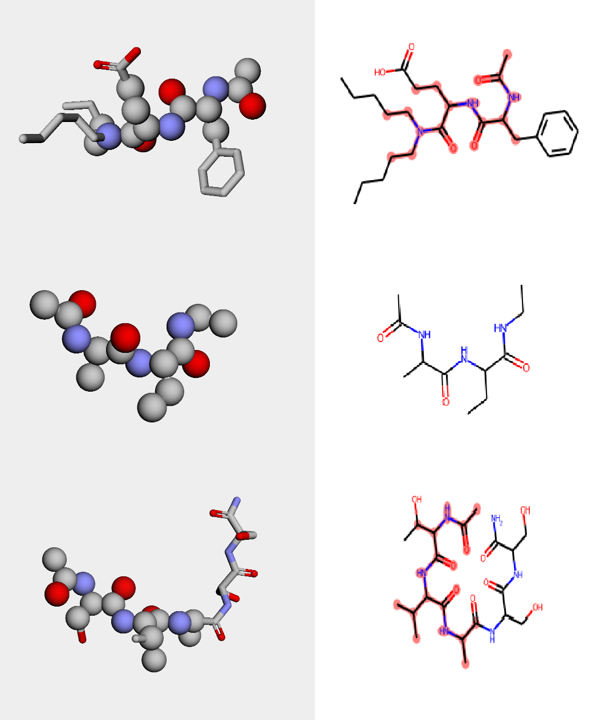
\includegraphics[scale=0.95]{trafo_py3d_2}

\caption{Two Visualizations of the mutation route with Py3Dmol (left column) and RDKit (right column). First and third row: Representation of the physical end states, left: spheres represent CC atoms, whereas non-CC atoms are shown in licorice representation; right: CC atoms are highlighted in red. Middle row: CC of the two end states.
}
\label{fig:py3dmol}
\end{figure}


\section{Scoring schemes}

Several scoring schemes have been implemented to assess and compare
the mutation routes proposed by the new algorithms.\\
1) Betweenness centrality: Betweenness centrality measures the number
of shortest paths going through a specific node \cite{Newman.2010}. More central atoms
will have a higher, atoms remote from
the CC will have a lower centrality coefficient. In particular, the last atom of a chain
has a coefficient of 0 because no path between two other atoms visits
the representing node. After each step, the node is removed from
the graph.
For avoiding undesired mutations, the maximum betweenness centrality
of all mutation steps is more decisive; hence, the average of the mean
as well as the maximum betweenness centrality of all removed nodes
is shown below.

\begin{figure}[H]
	
	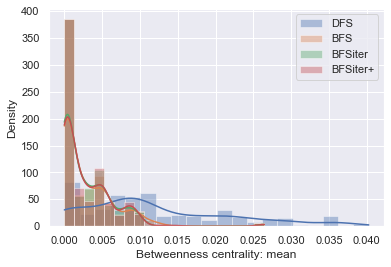
\includegraphics[scale=0.8]{betweenness_mean_all}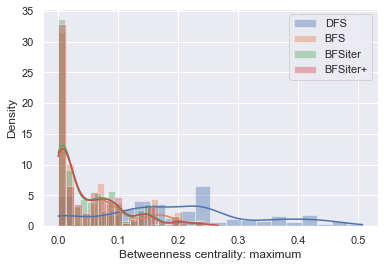
\includegraphics[scale=0.8]{betweenness_max_all}\caption{Betweenness centrality for the test ligands from the PDBbind-CN data set. Maximum and mean betweenness centrality are much higher for DFS than for all BFS-based mutation route algorithms. Curves are density estimates of the histograms.}
	\label{fig:betweenness_centrality}
\end{figure}

2) Closeness centrality: Closeness centrality of a specific node is
given by the inverted distances between this node and all other nodes
of the graph \cite{Newman.2010}. Similar to betweenness centrality, more 'important', central atoms have a higher closeness centrality, whereas atoms more distant from the CC have a lower
closeness centrality.
For using this centrality measure as a scoring function for the mutation
algorithms, the dummy region with the highest number of atoms (simply
because this is probably the most \textquoteleft interesting\textquoteright{}
one, it would also be possible to take the average of all dummy regions
etc.) is selected. The closeness centrality of each node representing a dummy atom for
the full graph representation, including all CC and dummy atoms, (i.e., all atoms, including already removed ones are used for calculating the statistics) is
computed. For a ‘good’ mutation route, the atoms should be removed approximately in ascending order of their closeness centrality: The first atoms should have a high distance to most of the other atoms and consequently low closeness centrality, whereas the ones removed later should be the more ‘important’ nodes with high closeness centrality. This is checked by computing Spearman's Rank correlation coefficients for each mutation route. The correlation between the order of mutation and closeness centrality is determined. A higher positive correlation coefficient shows that the
closeness centrality of the atoms removed is increasing and, thus, indicates a 'better' route. The computed correlation coefficients for all mutation paths are visualized via histograms. 

\begin{figure}[H]
	
	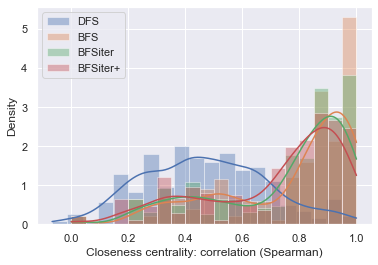
\includegraphics[scale=1.2]{closeness_spearman}
    \caption{Histogram showing the distribution of the Spearman's Rank correlation coefficients of the closeness centrality values computed for the test ligands from the PDBbind-CN data set. It was checked if the closeness centrality of the removed atoms increases during mutation. A 'good' mutation route should show an increase in closeness
centrality because at the beginning the atoms with a high distance
from the other atoms (and hence the CC atoms) and thus a low closeness centrality are removed. When atoms are removed with ascending closeness centrality --- which indicates a 'good' mutation route ---, this leads to a higher positive correlation.  Closeness centrality is computed for the full graph representation, including all CC and dummy atoms. Curves are density estimates of the histograms.}
	\label{fig:closeness_centrality}
\end{figure}


3) Ring-related scores: As stated above, the processing of ring structures
is of crucial importance and pronounced differences between DFS and
BFS occur. Four properties were calculated: The mean asymmetry at
ring opening was measured: After the first atom of a ring structure
is removed, usually two chains emerge. The length difference (i.e.,
the difference in atom number) of these two chains was measured. If
both chains are equally long, the asymmetry is 0. 

The 'asymmetry during ring disassembly'-score does not only evaluate
the first atom removed from a ring, but checks at each mutation step
involving a ring atom if asymmetric chains emerge.

The 'mean number of open rings' indicates how many ring structures
are opened on average, and the 'mean processing time of rings' determines
how many mutation steps it takes to process a ring completely (until
only one atom of the former ring structure is present).

Even using the new algorithms, it is possible 
that a \textquoteleft broken\textquoteright{} ring exists for several mutation steps
 because atoms from other areas of the dummy region (e.g.,
a longer chain) are processed before the ring continues to be processed. However, in contrast to DFS,
it should not happen that a ring near to the CC is opened, but some of its atoms are processed much later, and hence the mean and maximum time should be significantly shorter. 

To compare the mutation algorithms, calculation of the scoring functions for the selection of ligands from the PDBbind-CN data set was performed. 

In general, the computed statistics match the expectations. The range of betweenness centrality scores is much lower for BFS, suggesting that central nodes, i.e., atoms in a ring next to the common core, are processed last, whereas isolated ones, i.e., atoms at the final position of a chain, are processed preferably (fig. \ref{fig:betweenness_centrality}).
Likewise, the correlation between the order of mutation of an atom and its closeness centrality scores is higher for BFS-based approaches because atoms distant from the common core are visited only at the final iterations of the algorithms and so there is a stronger positive correlation between closeness centrality and  mutation order (fig. \ref{fig:closeness_centrality}). For many mutation routes, the correlation of the BFS approaches is almost perfect, i.e., near to one, whereas for DFS it is much lower.
All scoring functions show that the BFS-based algorithms tend to prune the molecule graph at positions more distant from the CC at the beginning of the processing, and rings are processed in a more systematic and 'symmetric' manner (fig. \ref{fig:ring_related}).

In the plots presenting the scoring-functions, all molecule combinations
from the PDBbind-CN data set were used. Thus, the selection of molecule pairs gives rise to CCs and dummy regions with entirely different properties (e.g., number of atoms and presence of cyclic structures) and many  'trivial' structures are over-represented. It could be insightful to use
only a subset (e.g., only molecules with dummy regions involving multiple
ring structures or a minimum number of dummy atoms) or to try even a larger selection from the PDBbind-CN database.




\begin{figure}
	
	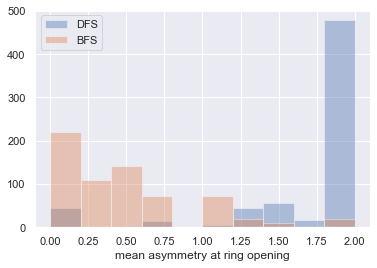
\includegraphics[scale=0.8]{mean_ass_beginn_bfs}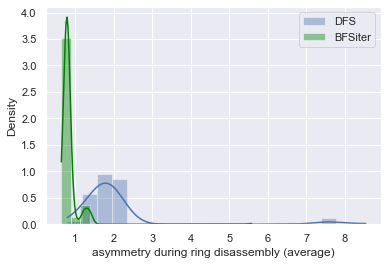
\includegraphics[scale=0.8]{mean_ass_total_onlyiter}
	
	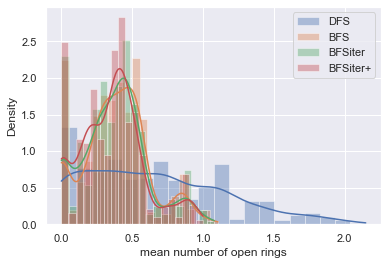
\includegraphics[scale=0.8]{mean_open_rings_all}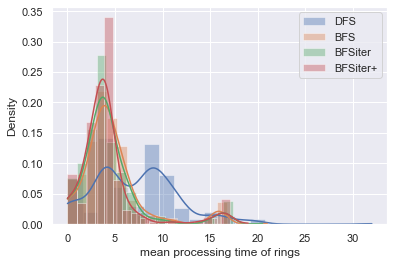
\includegraphics[scale=0.8]{mean_processing_all}
	
	\caption{Ring-related scores for the PDBbind-CN test set. upper row: left: difference in number of atoms in the emerging chains after first removal of a ring atom, a score of 0 means symmetric processing; right: difference in number of atoms in the emerging chains after removal of a ring atom, lower score means more symmetric processing; lower row: left: mean number of open rings in the test molecules after each processing step, lower score means that rings are processed sequentially and not in parallel; right: mean number of mutation steps until a ring is totally processed. Curves are density estimations of the emerging distributions.}
	\label{fig:ring_related}
\end{figure}



\section{Results for selected molecule pairs}

For a selection of small molecules taken from \cite{Loeffler.2018, Wieder.2022}, the relative solvation free energy differences were calculated  using {\trafo} with the old and the new mutation route algorithms. In particular, we studied the three pairs toluene/methane, 2-methylfuran/methane, and 2-methylindole/methane, as well as the
solvation free energy difference between 2-cyclopentyl-indole and 7-cyclopentyl-indole (2-/7-CPI). For the last case, the free energy differences were recomputed only for the new algorithms; however, earlier results using the old algorithm were used for comparison. This is one of the most interesting examples because the old CC generation, which searched for the CC including hydrogens without the improvements reported in 'Processing of hydrogen atoms', generated a smaller CC (fig. \ref{fig:cpi_comparison}). Thus, one would expect that for this example, differences should be especially pronounced.

Although these molecules are rather small and simple, they encompass some of the most interesting features, like rings. For instance, the mutation route for toluene is fundamentally different depending on the algorithm: the old algorithm starts next to the atom of the phenyl group that is connected to the methyl substituent --- which serves as the CC --- and processes the rest of the atoms in a chain-like manner. By contrast, the new one starts at the atom with maximum distance from the substituent and proceeds symmetrically until the CC is reached.
An overview of the molecules and the corresponding mutation routes is shown in figs. \ref{fig:all_paper_molecules} and \ref{fig:cpi_paper_molecule}.
The simulation results are averaged over four runs (except 2-CPI/7-CPI, for which only three runs were performed). 
For all these examples, the standard deviation is smaller using the new route finding algorithm and adapted settings for the generation of the CC (fig. \ref{fig:boxplot_small} and table \ref{tab:results_selection}).

\begin{table}
	\begin{tabular}{|>{\centering}p{5.5cm}|>{\centering}p{3.5cm}|>{\centering}p{3.5cm}|}
		\hline 
		mutation partners & old algorithm (DFS) & new algorithm (BFS) \tabularnewline
		\hline 
		toluene/methane & 2.02 $ \pm $ 0.21 & 2.05 $ \pm $ 0.04 \tabularnewline
		\hline 
		2-methylfuran/methane & 1.47 $ \pm $ 0.24 & 1.60 $ \pm $ 0.16 \tabularnewline
		\hline 	
		2-methyl-1H-indole/methane & 7.85 $ \pm $ 0.23 & 8.20 $ \pm $ 0.13 \tabularnewline
		\hline 	
		
	\end{tabular}\caption{results for a selection of mutation partners }
 \label{tab:results_selection}
\end{table}

\begin{figure}
	
	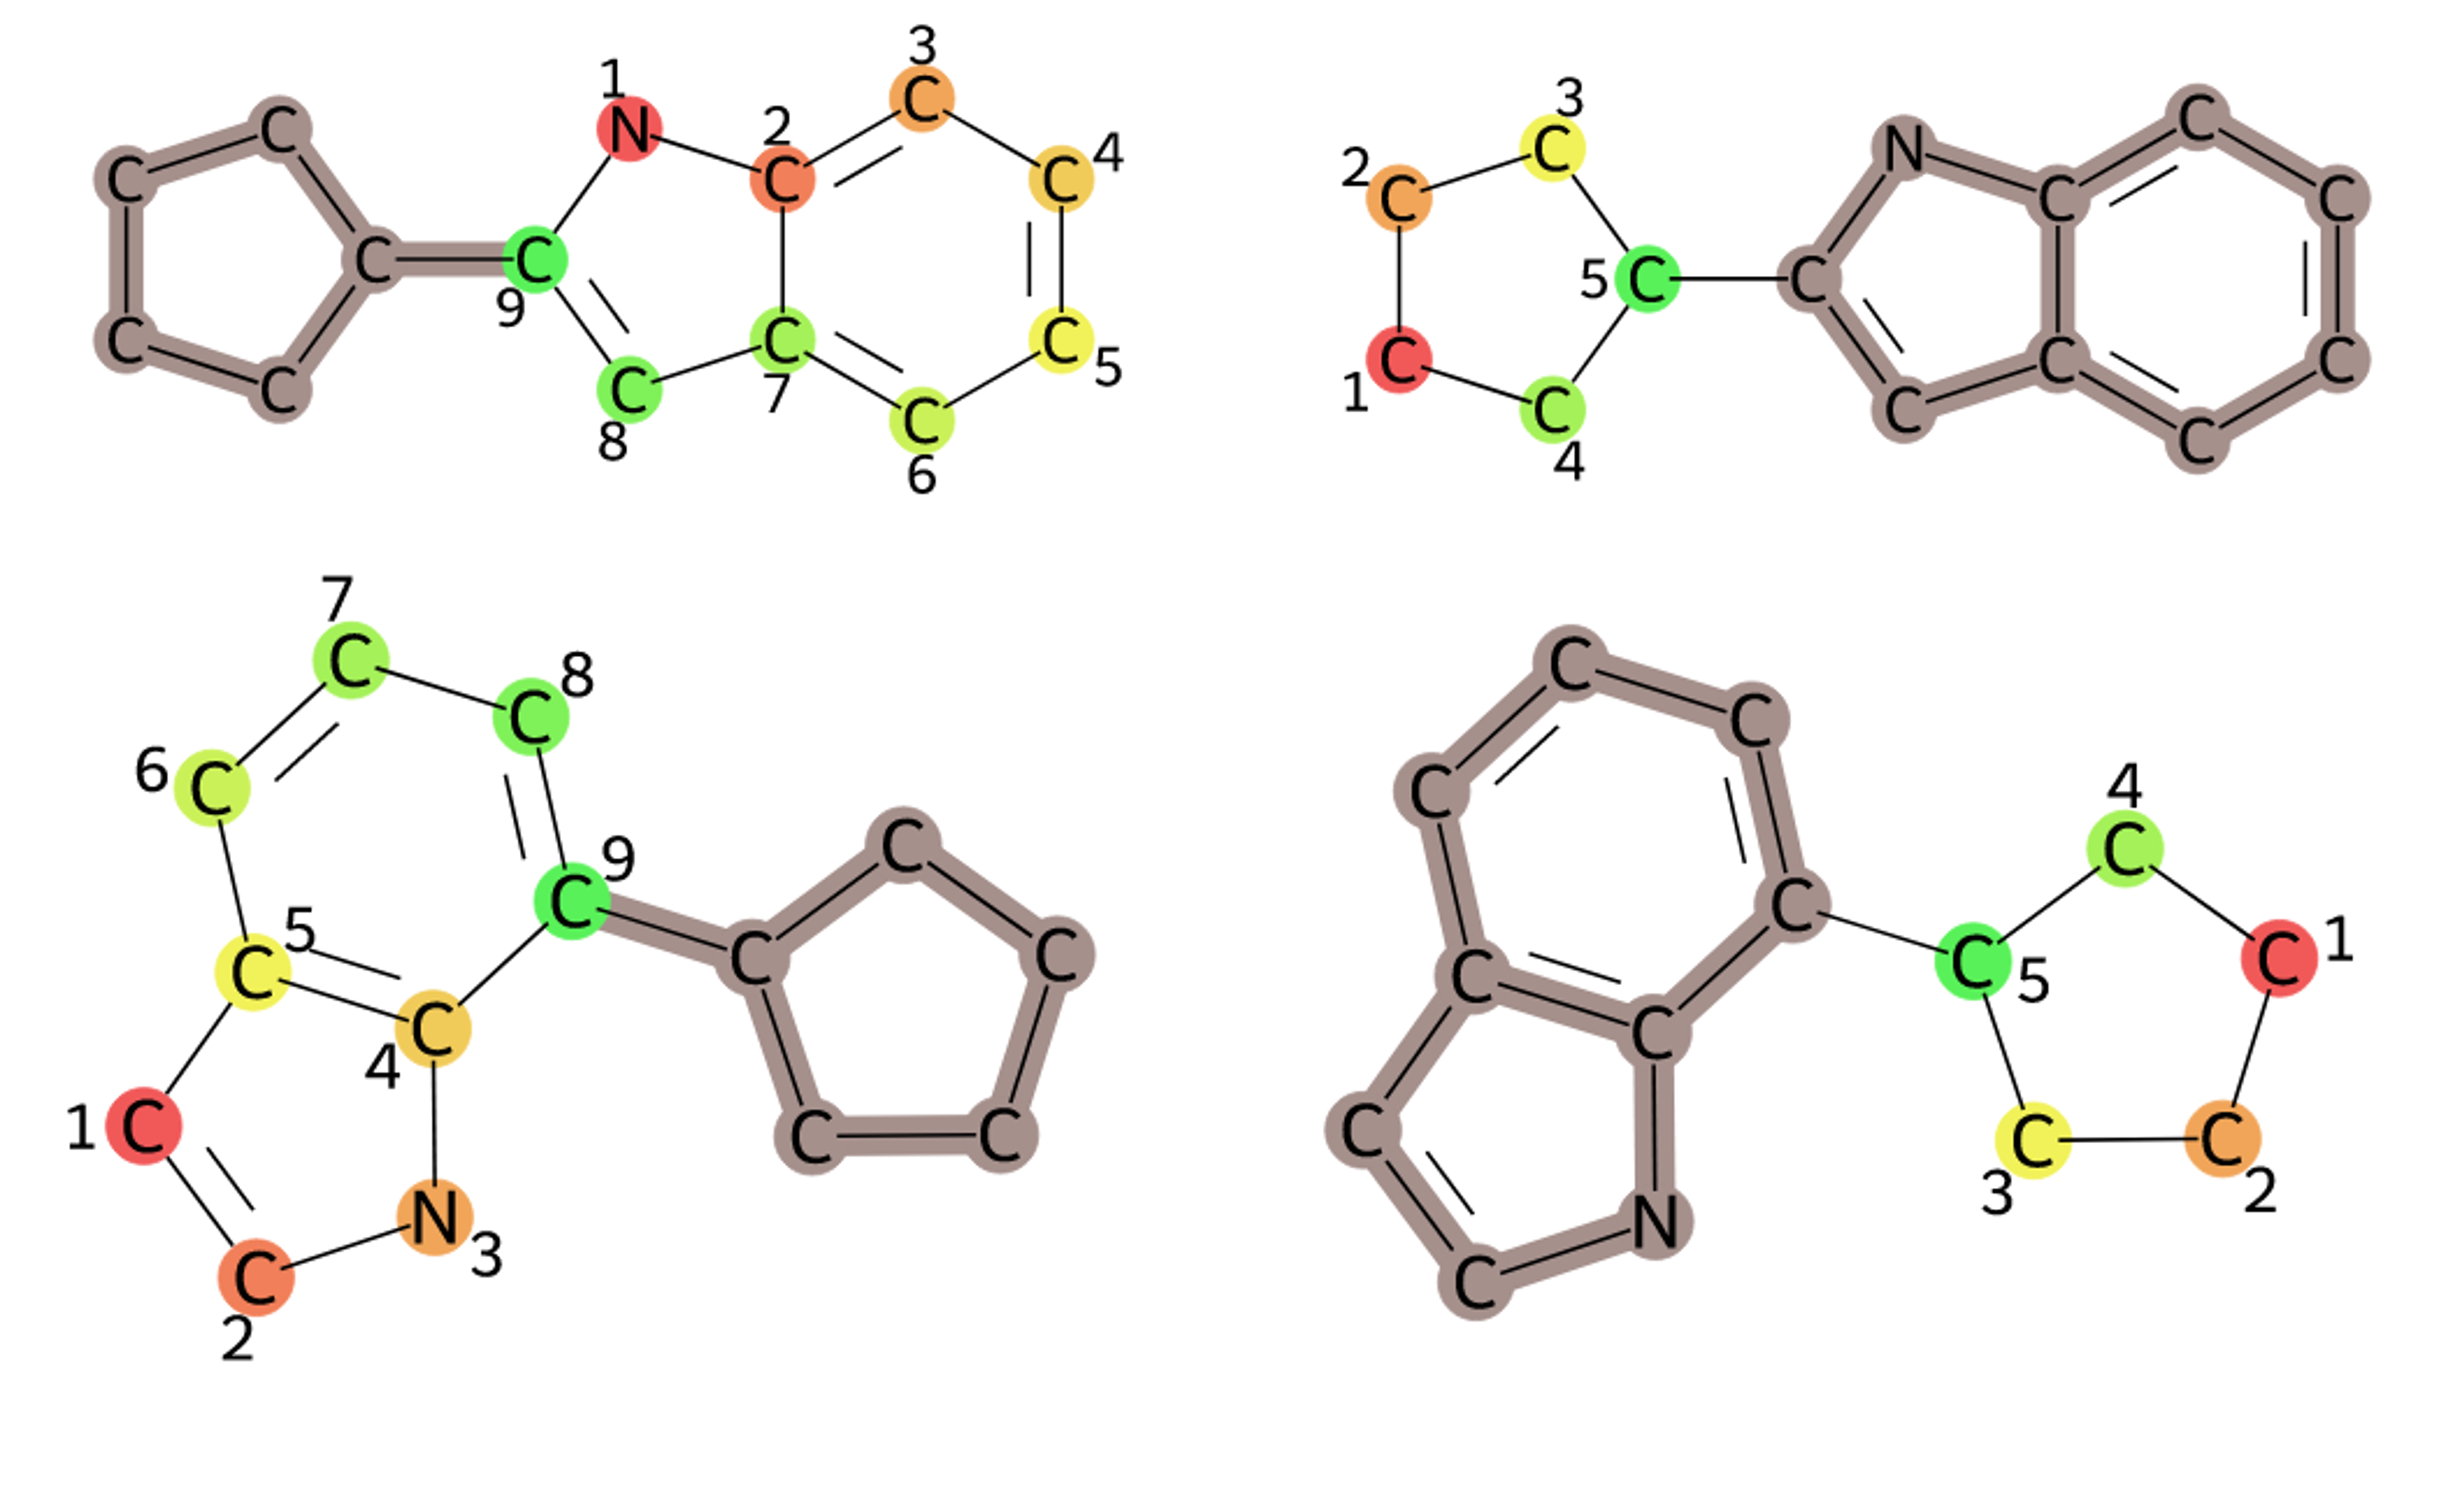
\includegraphics[scale=0.50]{cpi_old_new}
	\caption{mutation routes for 2-cyclopentylindole (upper row)/7-cyclopentylindole (lower row); left: small CC with DFS-algorithm; right: bigger CC with BFS-algorithm; CC in dark; the smaller CC is obtained when hydrogens are not removed before the computation of the maximum common substructure (it should be noted that in this case even further manual post-processing is necessary because one atom of the indole is also attached to the CC)}
	\label{fig:cpi_comparison}
\end{figure}



\begin{figure}
	
	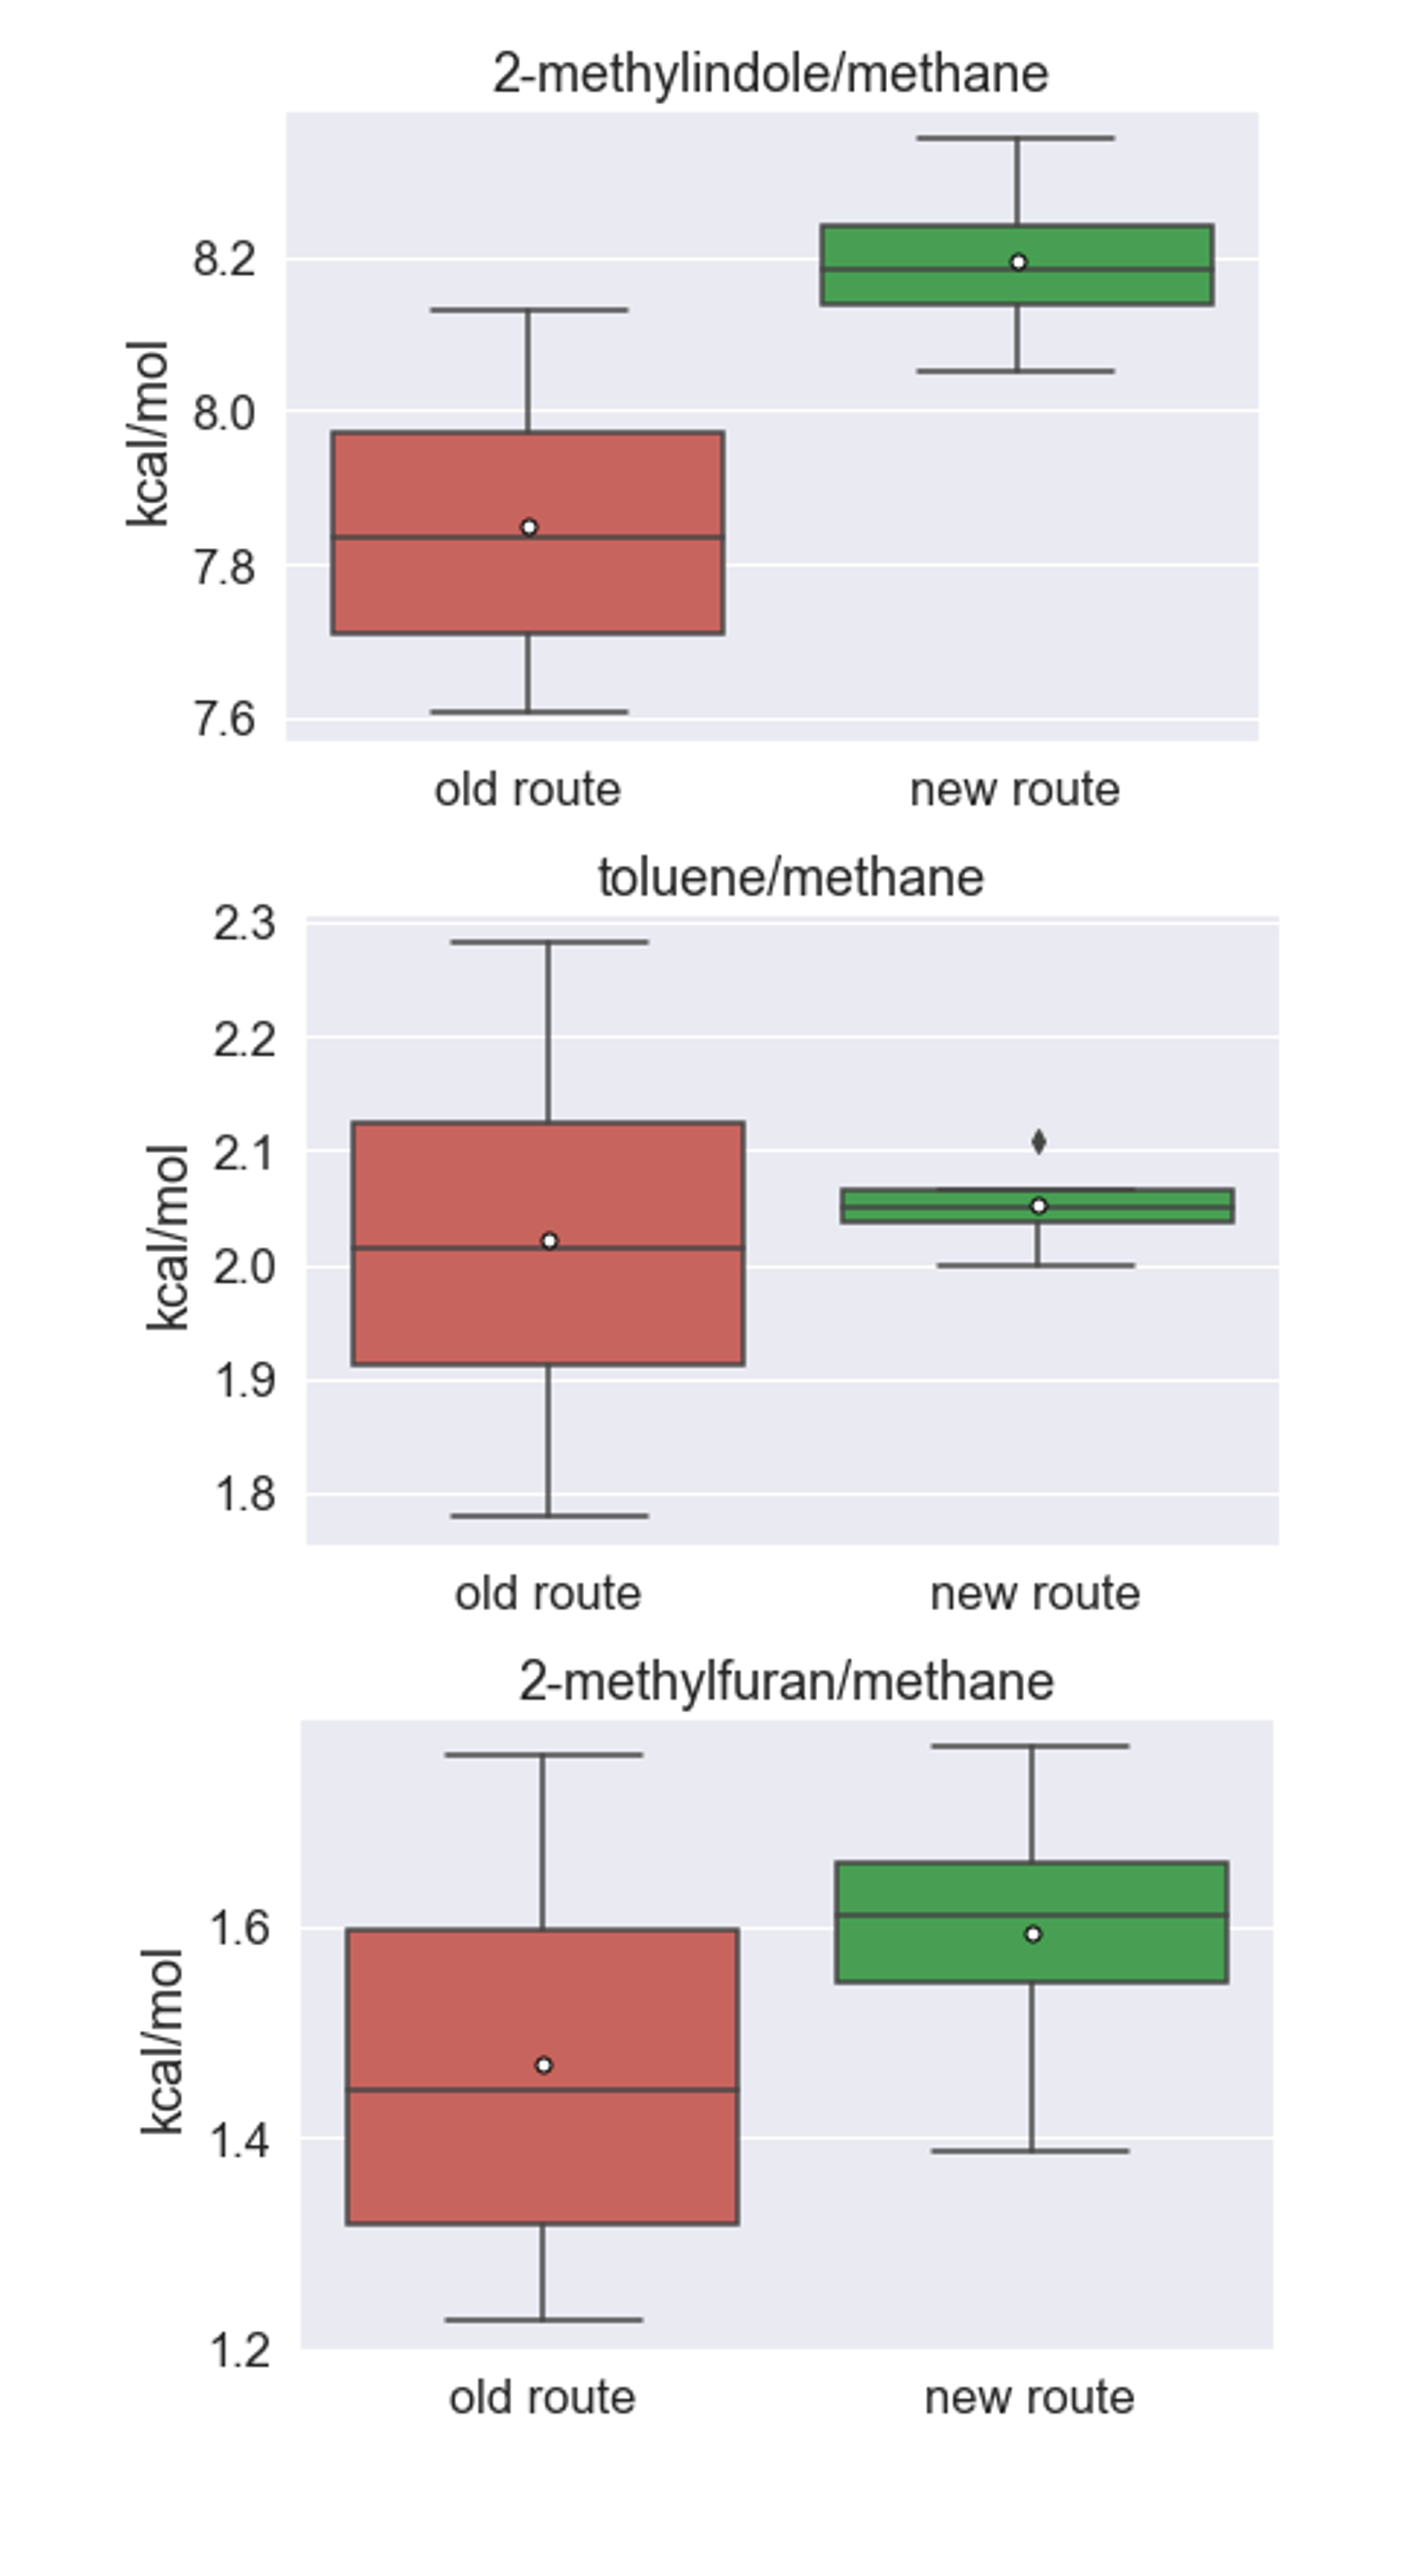
\includegraphics[scale=0.65]{results_3pairs1}
	\caption{comparison of results for mutating 2-methylindole, toluene and 2-methylfuran to methane.}
	\label{fig:boxplot_small}
\end{figure}


For the 2-/7-CPI-transformation, a relative free energy difference of $-1.55 \pm  0.10$ kcal/mol is computed using the CC and the route proposed by the new algorithms. In \cite{Fleck.2021}, for this transformation, $-1.43  \pm $ 0.30 kcal/mol was determined with the smaller cyclopentane-X CC. It can be assumed that the differences between the old and new mutation route are even more pronounced because in \cite{Fleck.2021} the calculations were repeated five times and averaged, in contrast to only three replicates for the run with the new mutation route. 
Of course, a direct comparison with the same number of replicates would be advantageous to quantify the improvement, but in any case, the change in standard deviation is remarkable.
Calculation of the absolute free energy differences of both molecules yield $-1.58  \pm  0.30$~kcal/mol. This indicates that the new route not only provides a smaller error, but also leads to a more accurate result.

However, probably the greatest advantage is that the mutation route for the new, bigger CC needs fewer states (only five in contrast to nine heavy atoms have to be mutated). 




\begin{figure}[h]
	\centering
	\subfigure[toluene/vacuum old]{%
		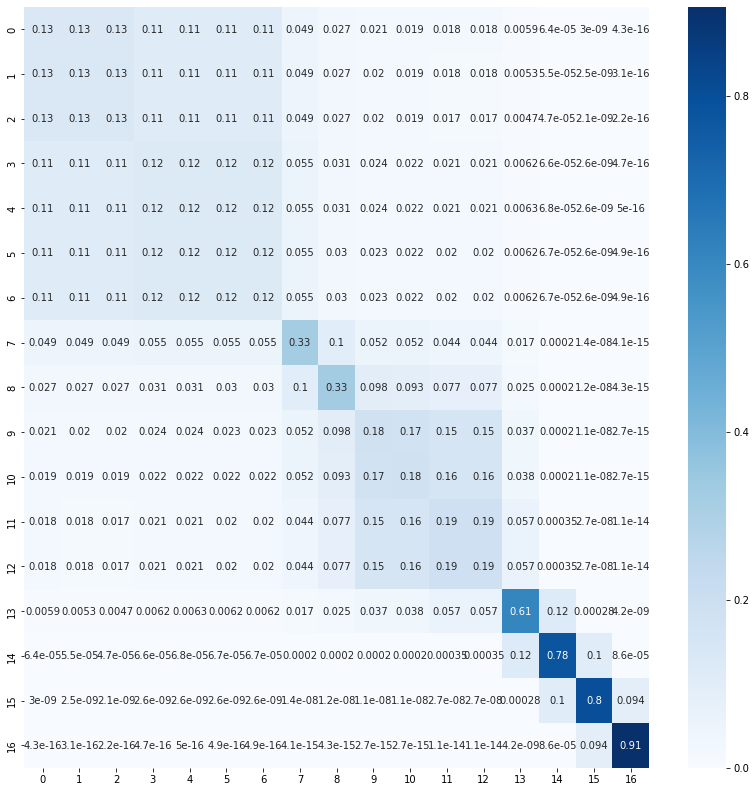
\includegraphics[width=0.5\textwidth]{overlap_vacuum_toluene_old_v2}%
		\label{fig:v_toluene_old}%
	}\hfil
	\subfigure[toluene/vacuum new]{%
		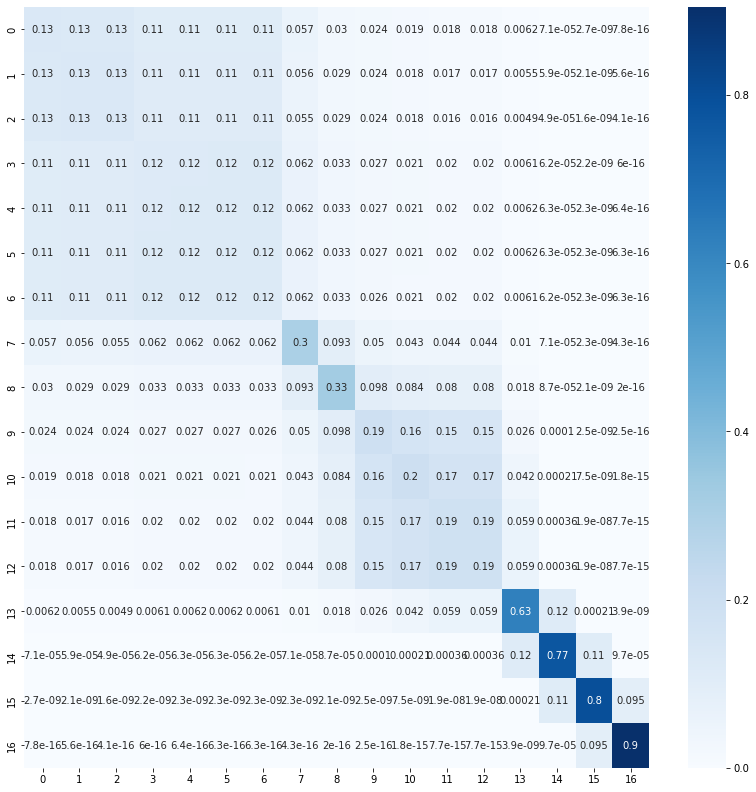
\includegraphics[width=0.5\textwidth]{overlap_vacuum_toluene_new_v2}%
		\label{fig:v_toluene_new}%
	}
	
	\subfigure[toluene/waterbox old]{%
		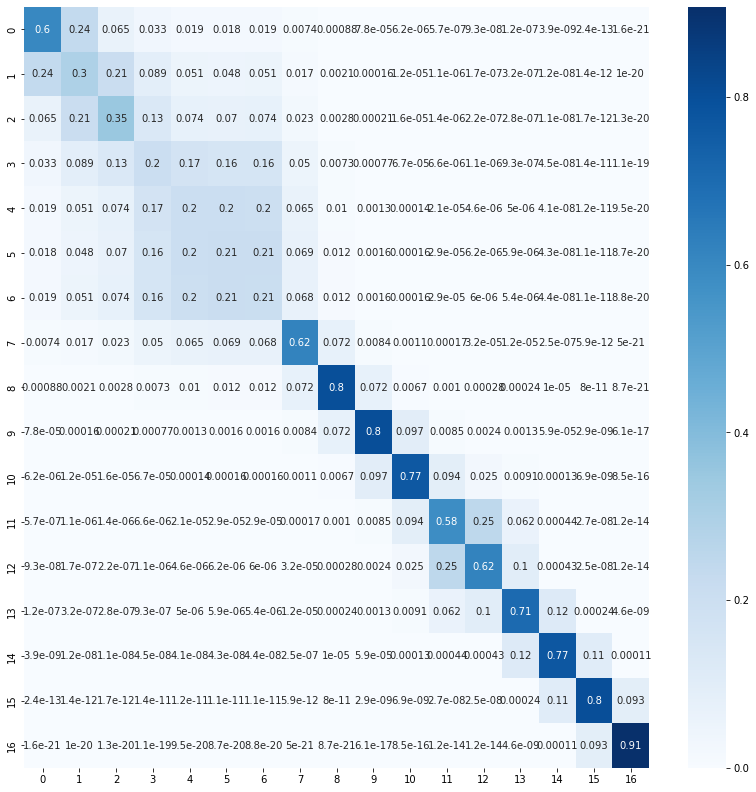
\includegraphics[width=0.5\textwidth]{overlap_waterbox_toluene_old_v2}%
		\label{fig:w_toluene_old}%
	}\hfil
	\subfigure[toluene/waterbox new]{%
		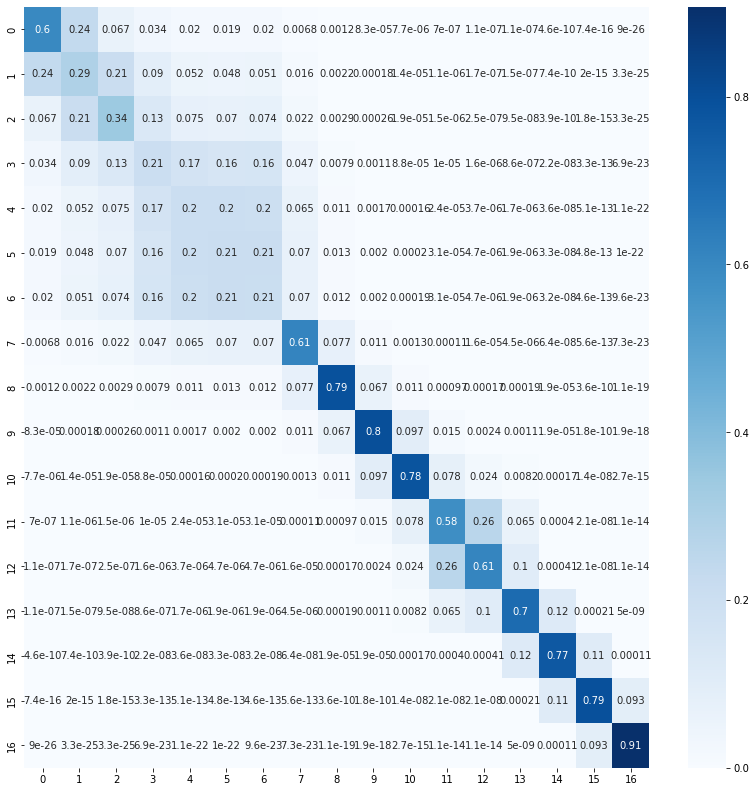
\includegraphics[width=0.5\textwidth]{overlap_waterbox_toluene_new_v2}%
		\label{fig:w_toluene_new}%
	}
	
	\caption{Overlap plots for toluene $\mathrm{\rightarrow}$ methane: upper row: vacuum, lower row: water box; left: old mutation algorithm, right: new mutation algorithm}
	\label{fig:toluene_overlaps}
\end{figure}


\begin{figure}[h]
	\centering
	\subfigure[toluene/vacuum old]{%
		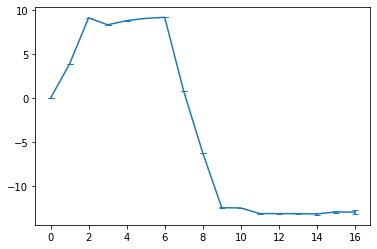
\includegraphics[width=0.55\textwidth]{states_toluene_vacuum_old_v2.png}%
		\label{fig:v_toluene_old_state}%
	}\hfil
	\subfigure[toluene/vacuum new]{%
		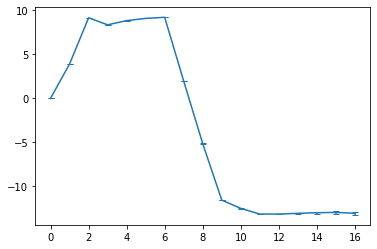
\includegraphics[width=0.55\textwidth]{states_toluene_vacuum_new_v2.png}%
		\label{fig:v_toluene_new_state}%
	}
	
	\subfigure[toluene/waterbox old]{%
		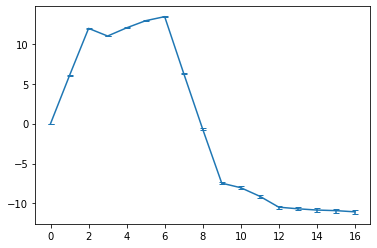
\includegraphics[width=0.55\textwidth]{states_toluene_water_old_v2.png}%
		\label{fig:w_toluene_old_state}%
	}\hfil
	\subfigure[toluene/waterbox new]{%
		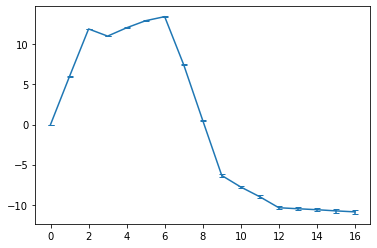
\includegraphics[width=0.55\textwidth]{states_toluene_water_new_v2.png}%
		\label{fig:w_toluene_new_state}%
	}
	
	\caption{free energy differences per state for toluene $\mathrm{\rightarrow}$ methane}
	\label{fig:toluene_states}
\end{figure}

\begin{figure}[h]
	\centering
	\subfigure[toluene/vacuum old]{%
		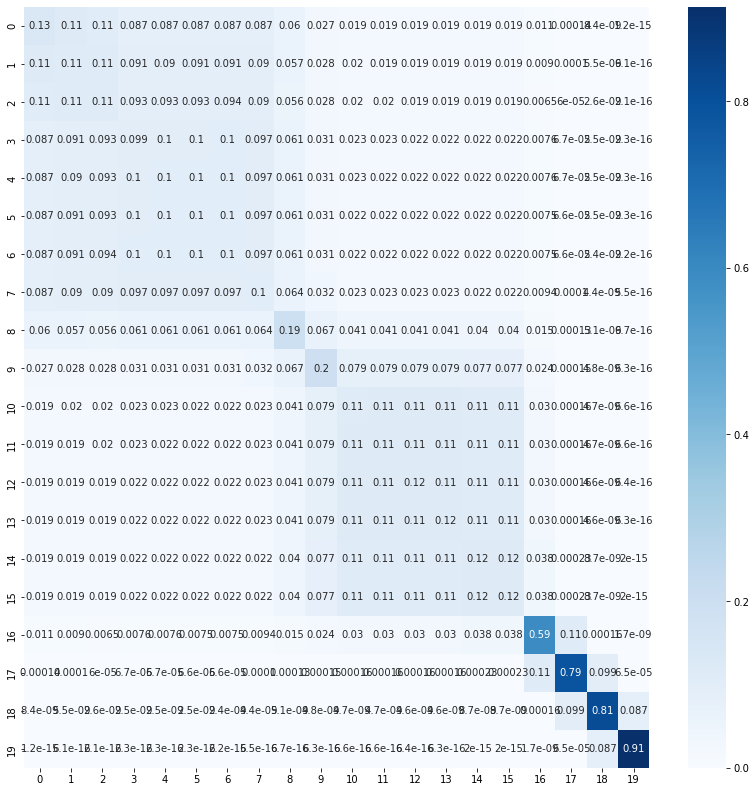
\includegraphics[width=0.5\textwidth]{overlap_vacuum_methylindole_old_v2}%
		\label{fig:v_methylindole_old}%
	}\hfil
	\subfigure[toluene/vacuum new]{%
		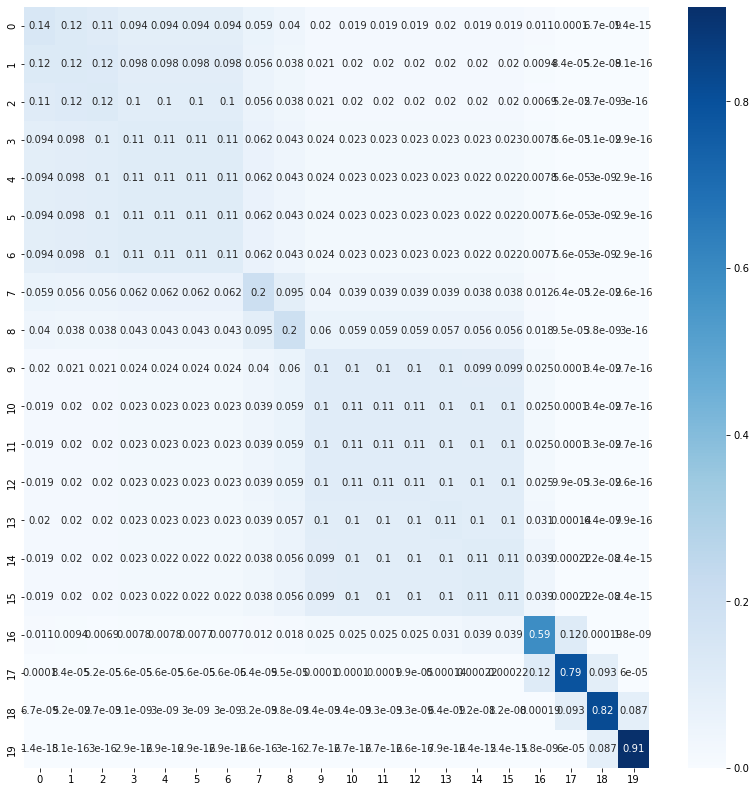
\includegraphics[width=0.5\textwidth]{overlap_vacuum_methylindole_new_v2}%
		\label{fig:v_methylindole_new}%
	}
	
	\subfigure[toluene/waterbox old]{%
		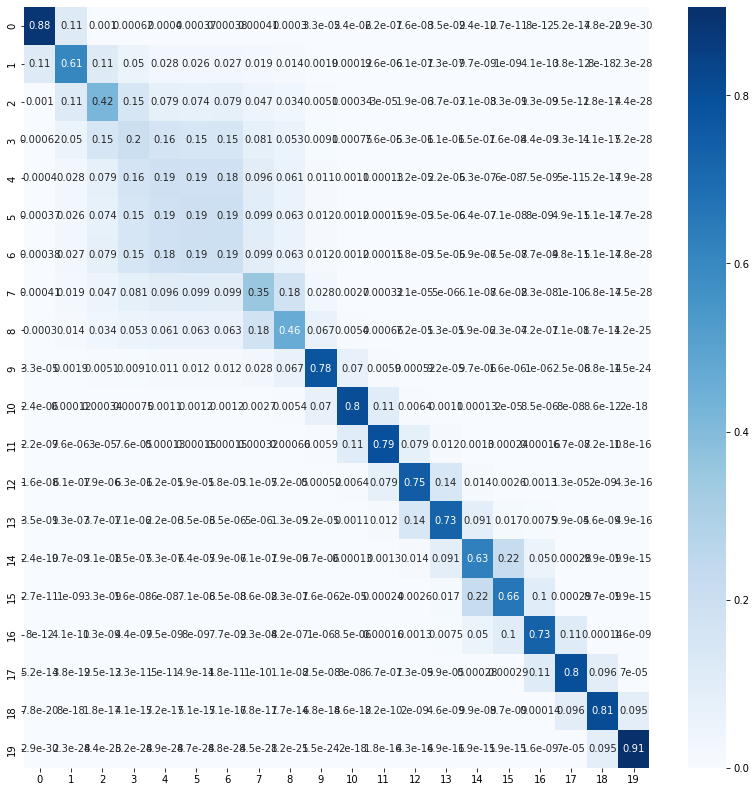
\includegraphics[width=0.5\textwidth]{overlap_waterbox_methylindole_old_v2}%
		\label{fig:w_methylindole_old}%
	}\hfil
	\subfigure[toluene/waterbox new]{%
		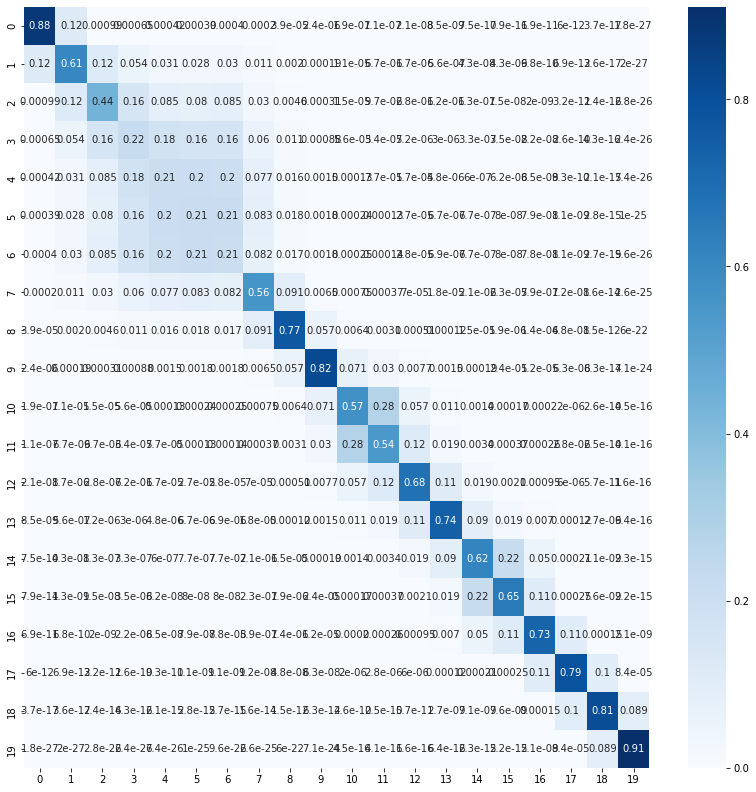
\includegraphics[width=0.5\textwidth]{overlap_waterbox_methylindole_new_v2}%
		\label{fig:w_methylindole_new}%
	}
	
	\caption{Overlap plots for 2-methyl-1H-indole $\mathrm{\rightarrow}$ methane: upper row: vacuum, lower row: water box; left: old mutation algorithm, right: new mutation algorithm}
	\label{fig:methylindole_overlaps}
\end{figure}


\begin{figure}[!htb]
	
	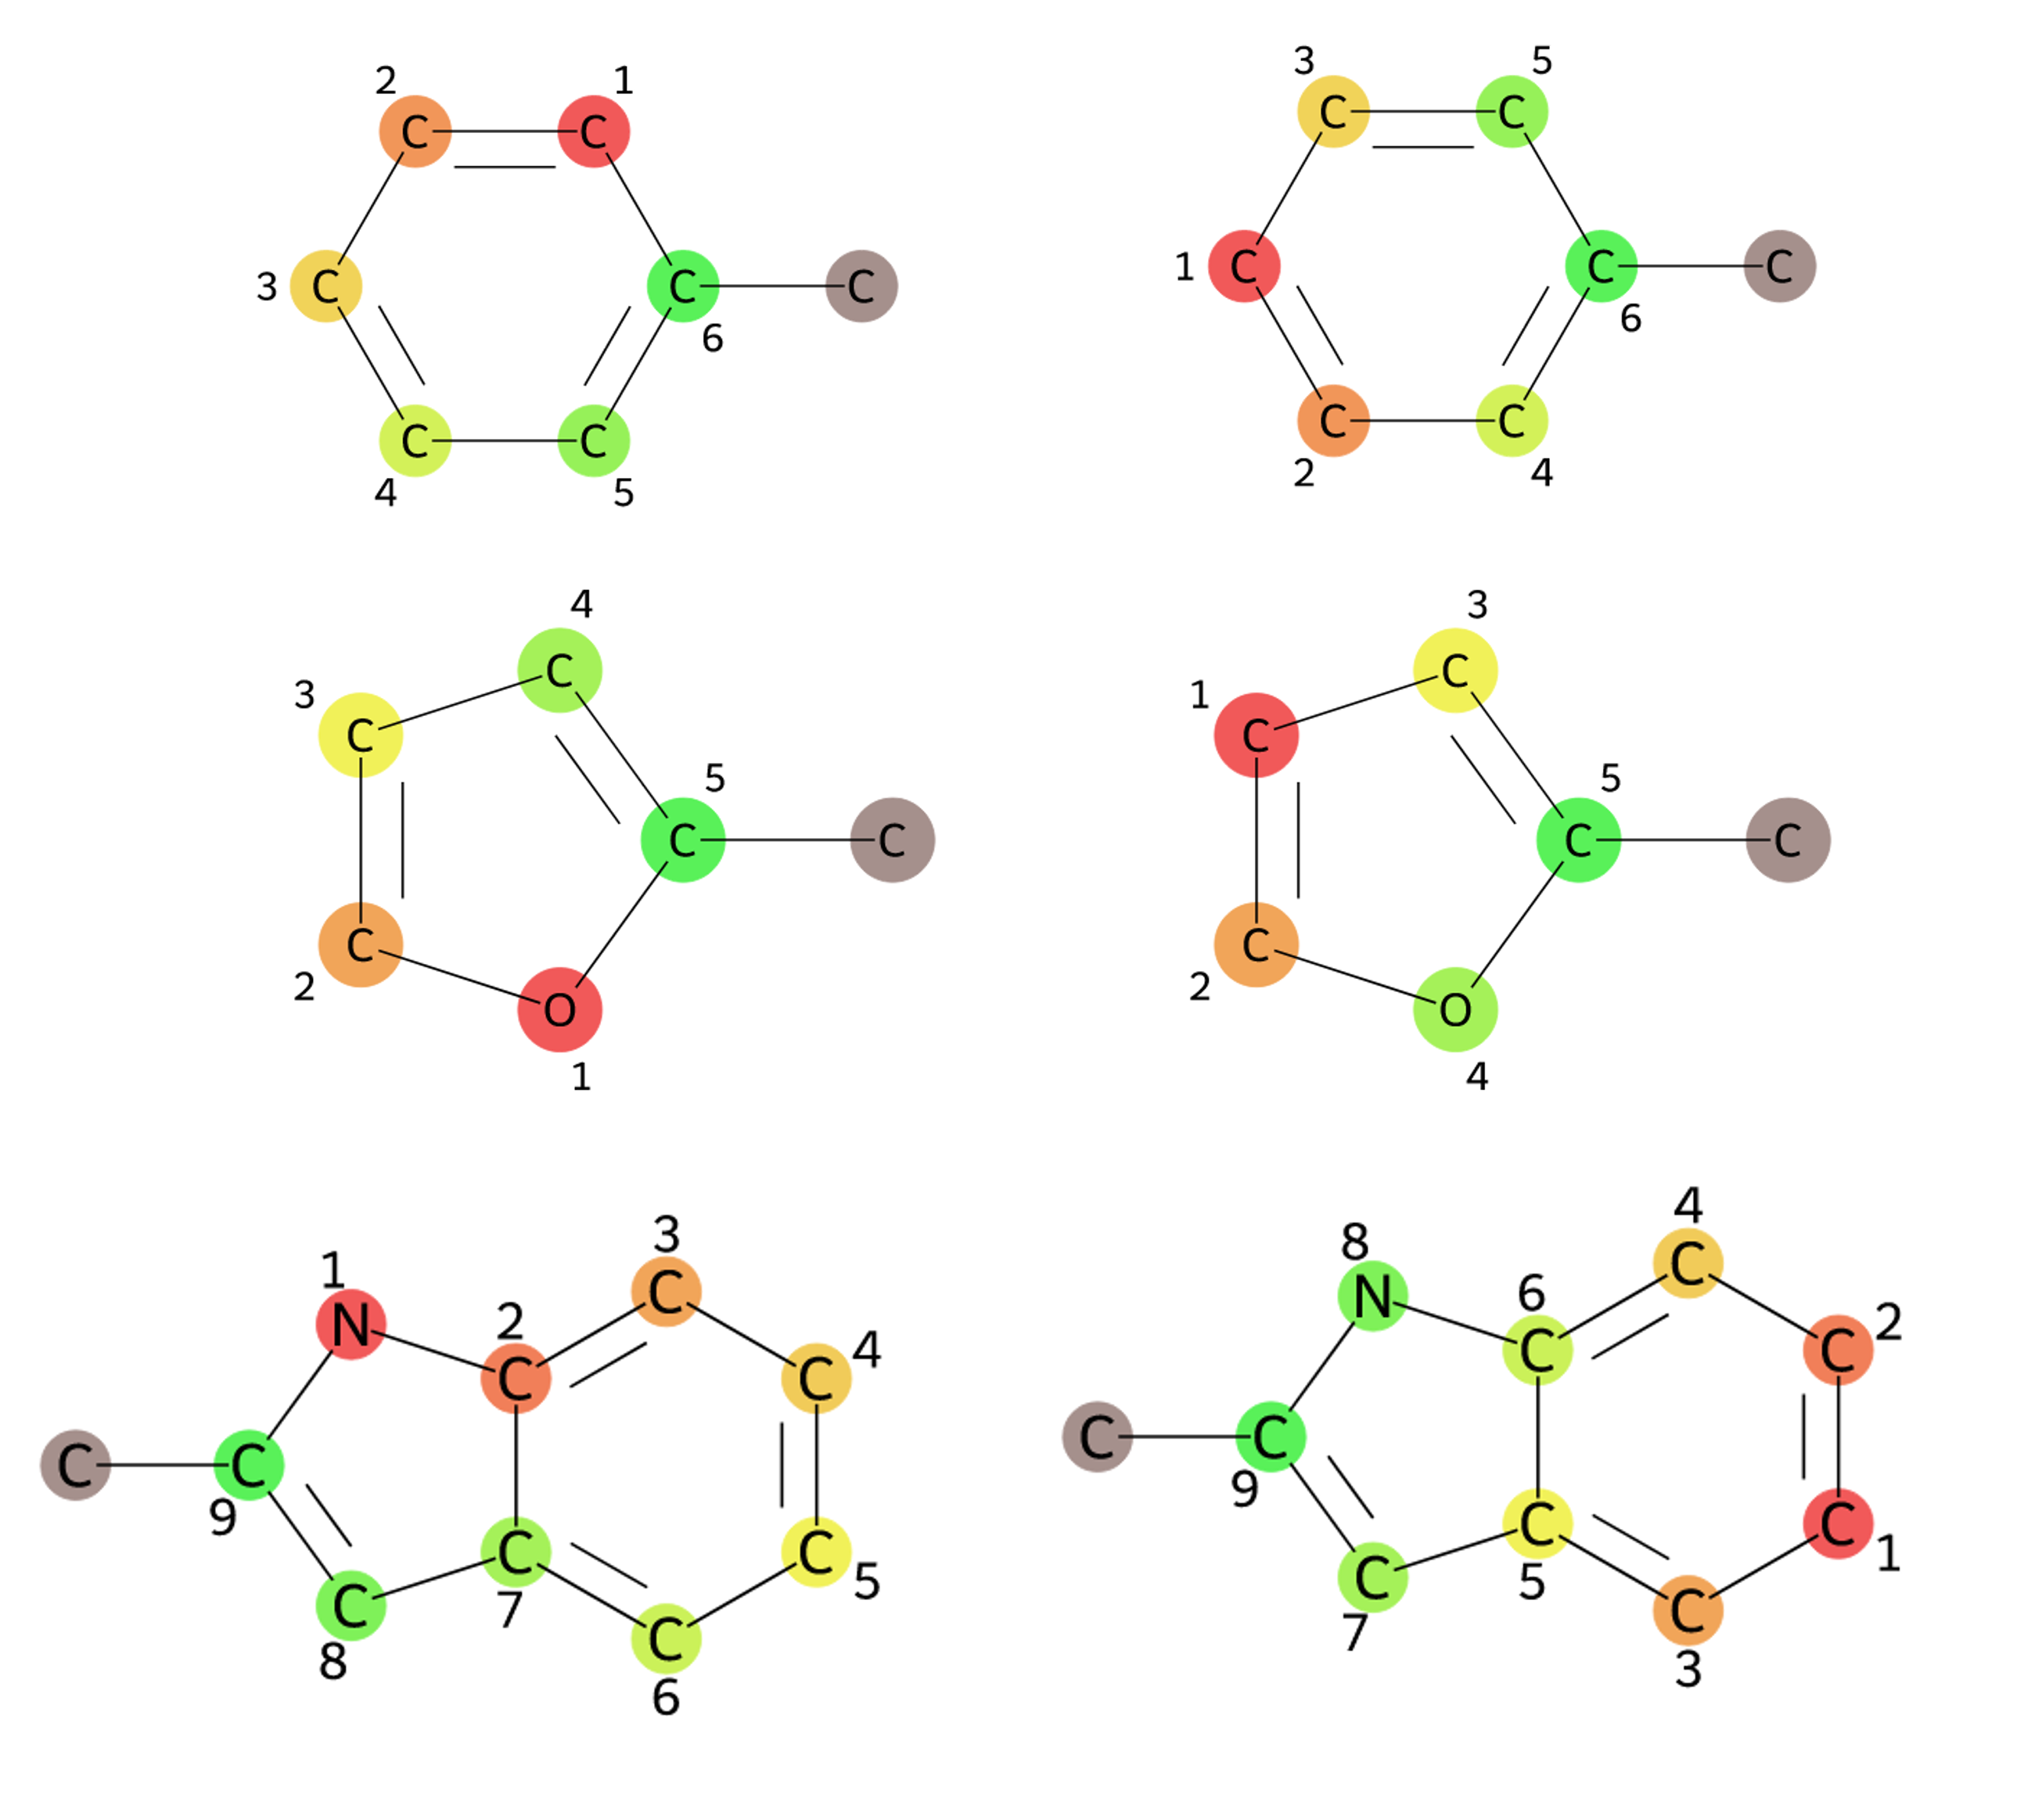
\includegraphics[scale=0.75]{paper_routes1a}\caption{left: DFS-algorithm; right: BFS-algorithm; CC in dark; from top to bottom row: mutation routes for toluene/methane, 2-methylfuran/methane, 2-methylindole/methane}
	\label{fig:all_paper_molecules}
\end{figure}


\begin{figure}[!htb]
	
	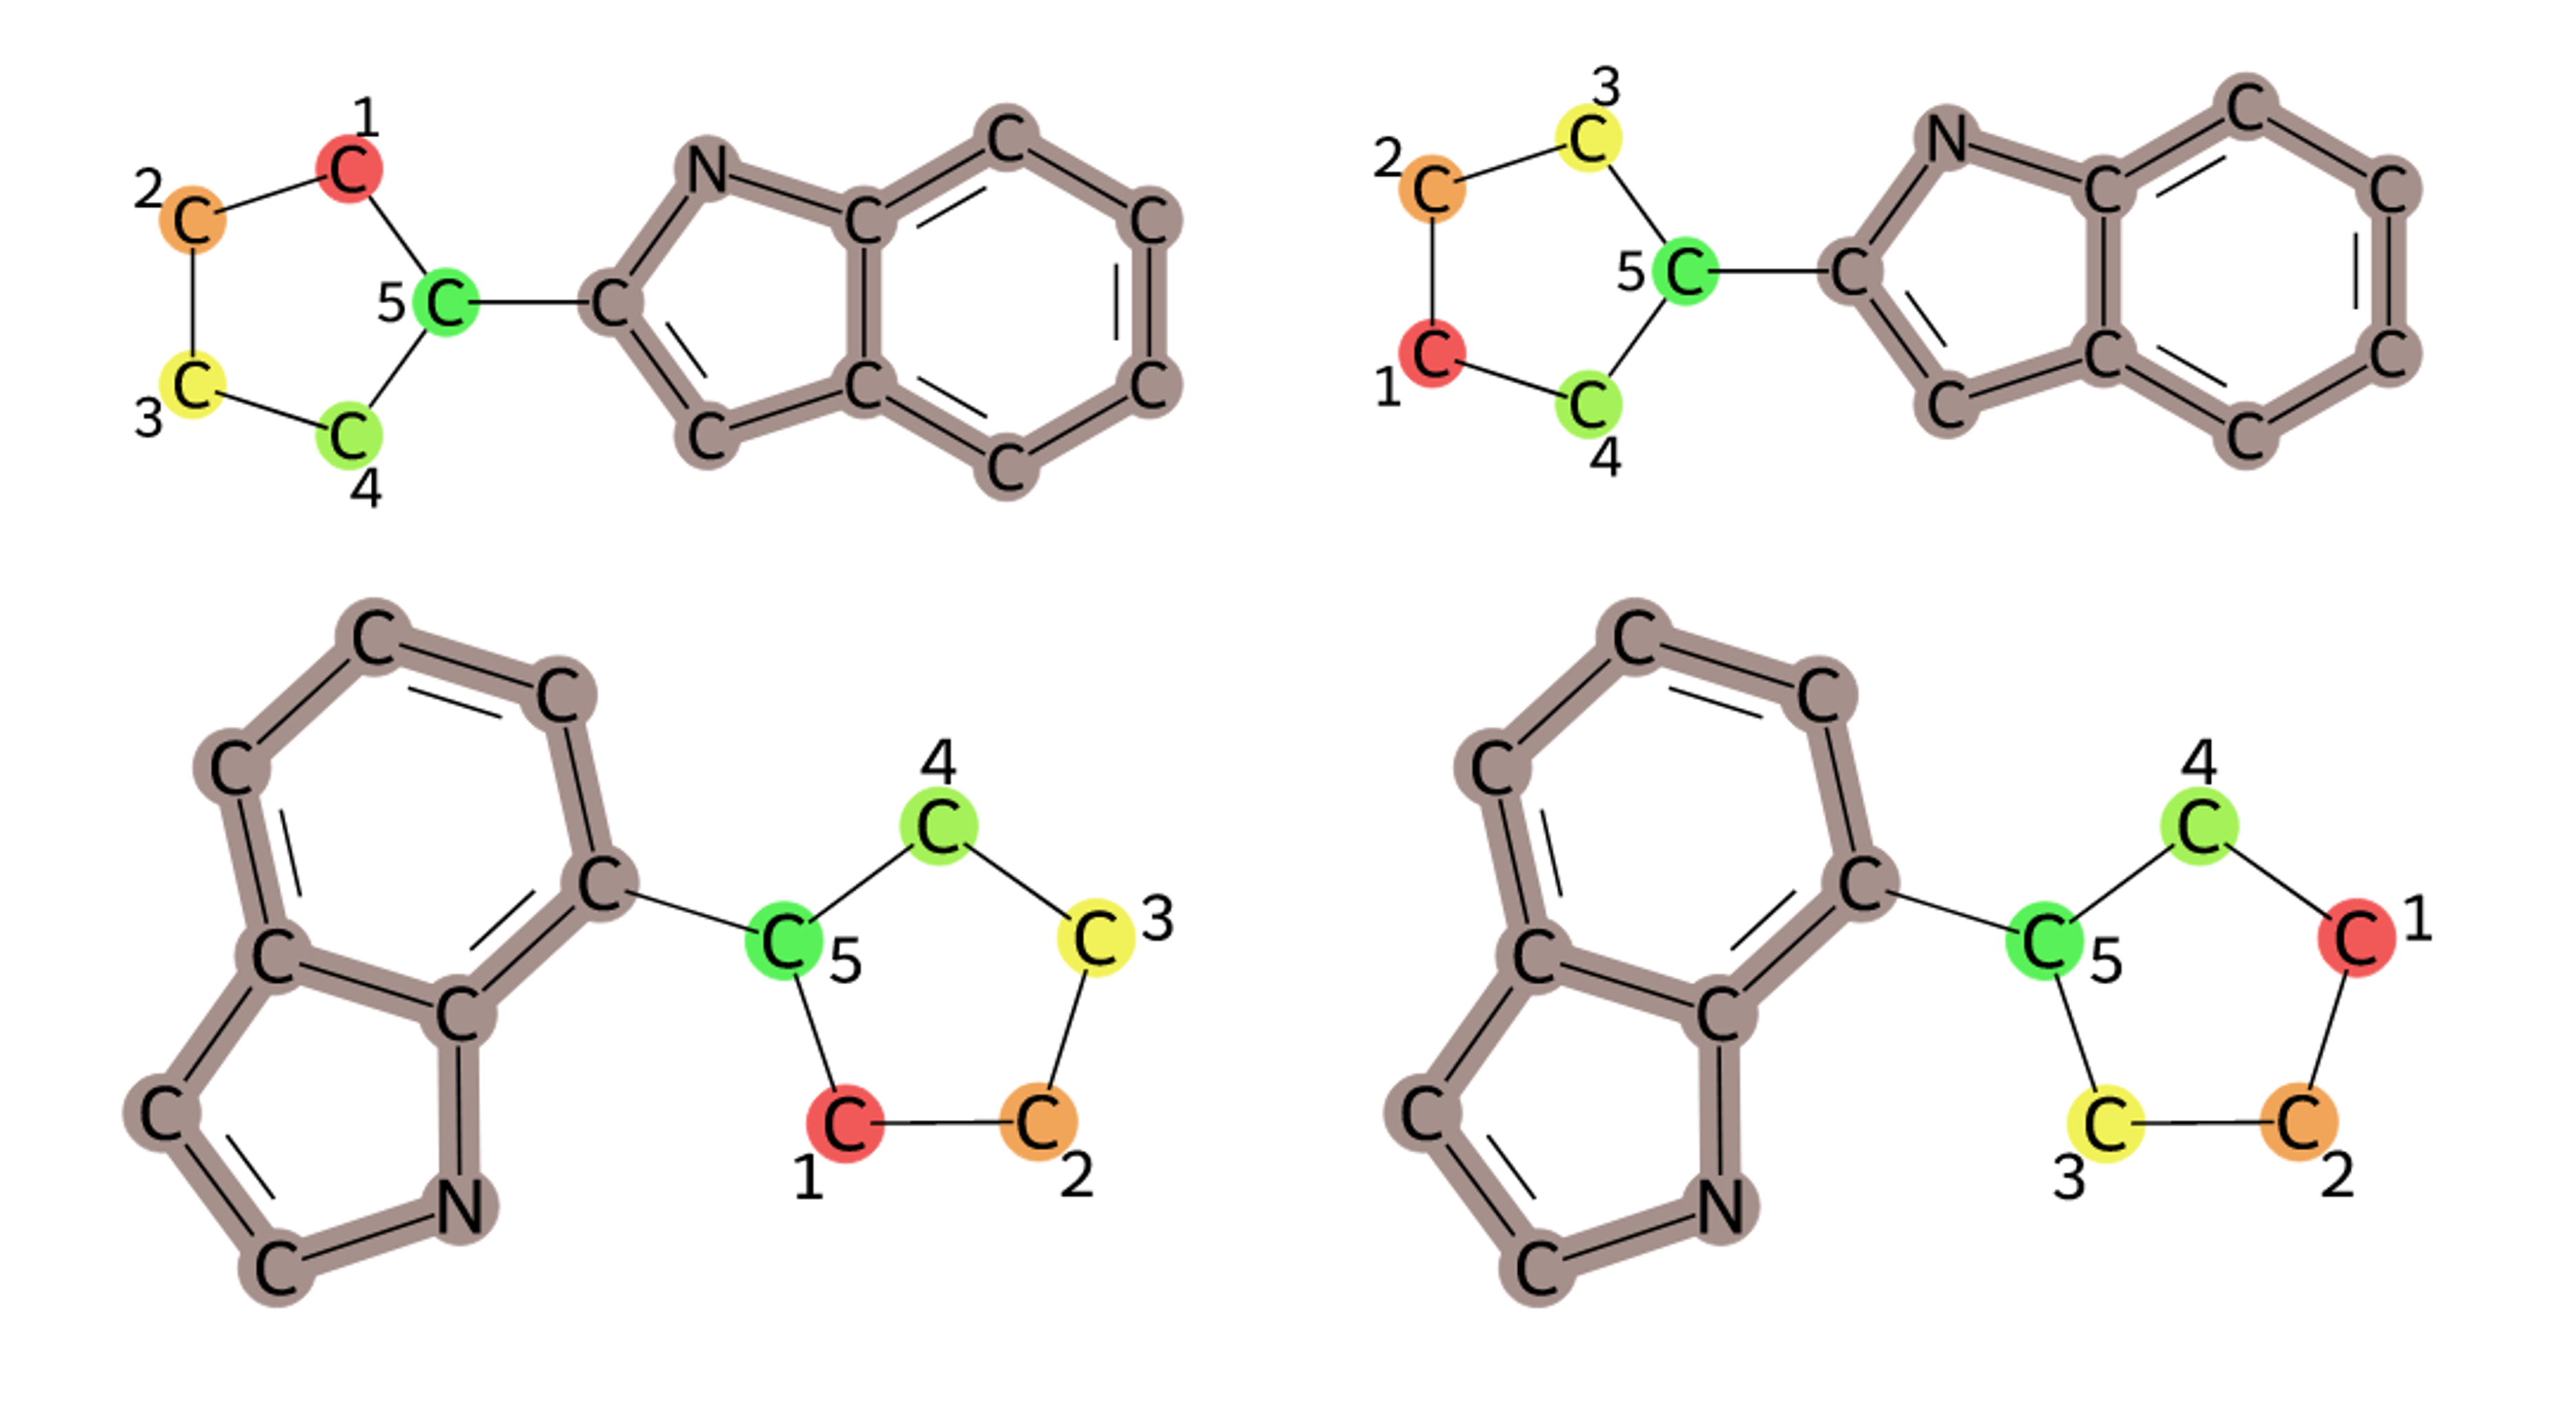
\includegraphics[scale=0.55]{paper_routes1b}\caption{left: DFS-algorithm; right: BFS-algorithm; CC in dark; mutation routes for 2-cyclopentylindole/7-cyclopentylindole}
	\label{fig:cpi_paper_molecule}
\end{figure}


An additional means for detecting differences between the outcome of the mutation algorithms is to compare runs of different sampling length. 
The results of the MD runs set up with {\trafo} can be evaluated using the functions of the MBAR class of \texttt{pymbar} \cite{Shirts.2008}. Python scripts were written to evaluate the computed free energy differences for different simulation lengths. There are two crucial parameters: the reduced potential energy of an uncorrelated configuration $n$ at a specific state $k$ (\texttt{u\_kn}) and the number of uncorrelated snapshots $n$ (\texttt{N\_k}). By removing the same number of configurations at each state k and adjusting (\texttt{N\_k}) accordingly, shorter simulations were generated artificially.
In \ref{fig:toluene_short}, \ref{fig:methylfuran_short} and \ref{fig:methylindole_short}, a comparison between old and new route for molecule pairs consisting of toluene, 2-methylfuran, 2-methyl-1H-indole and methane is presented. The mean of the calculated free energy differences as well as the standard deviation is shown. In \ref{fig:cpi_short}, free energy differences for the 2-CPI-mutations at the two conditions (water box and vacuum) are visualized. 
As expected, for longer simulation lengths the standard deviation decreases, whereas very short simulation lengths (i.e., a very low number of configuration snapshots as input for the MBAR computations using \texttt{pymbar}) lead to unreliable results. However, looking at the evolution of the free energy difference mean value and standard deviation, it is difficult to confirm the superiority of one of the mutation routes for these three transformations or to indicate a sufficient minimum simulation length.
Furthermore, the \texttt{pymbar}-package \cite{Shirts.2008} allows the computation of overlap plots. Figs. \ref{fig:toluene_overlaps}, \ref{fig:toluene_states}, and \ref{fig:methylindole_overlaps} show overlap plots and the change of free energy difference of one run between the states for toluene $\mathrm{\rightarrow}$ methane and overlap plots for 2-methyl-1H-indole. In the case of 2-methyl-1H-indole (the mutation involves processing of a double ring),  significant differences for the water box between the old and new algorithm are discernible.



\begin{figure}[!htb]
	
	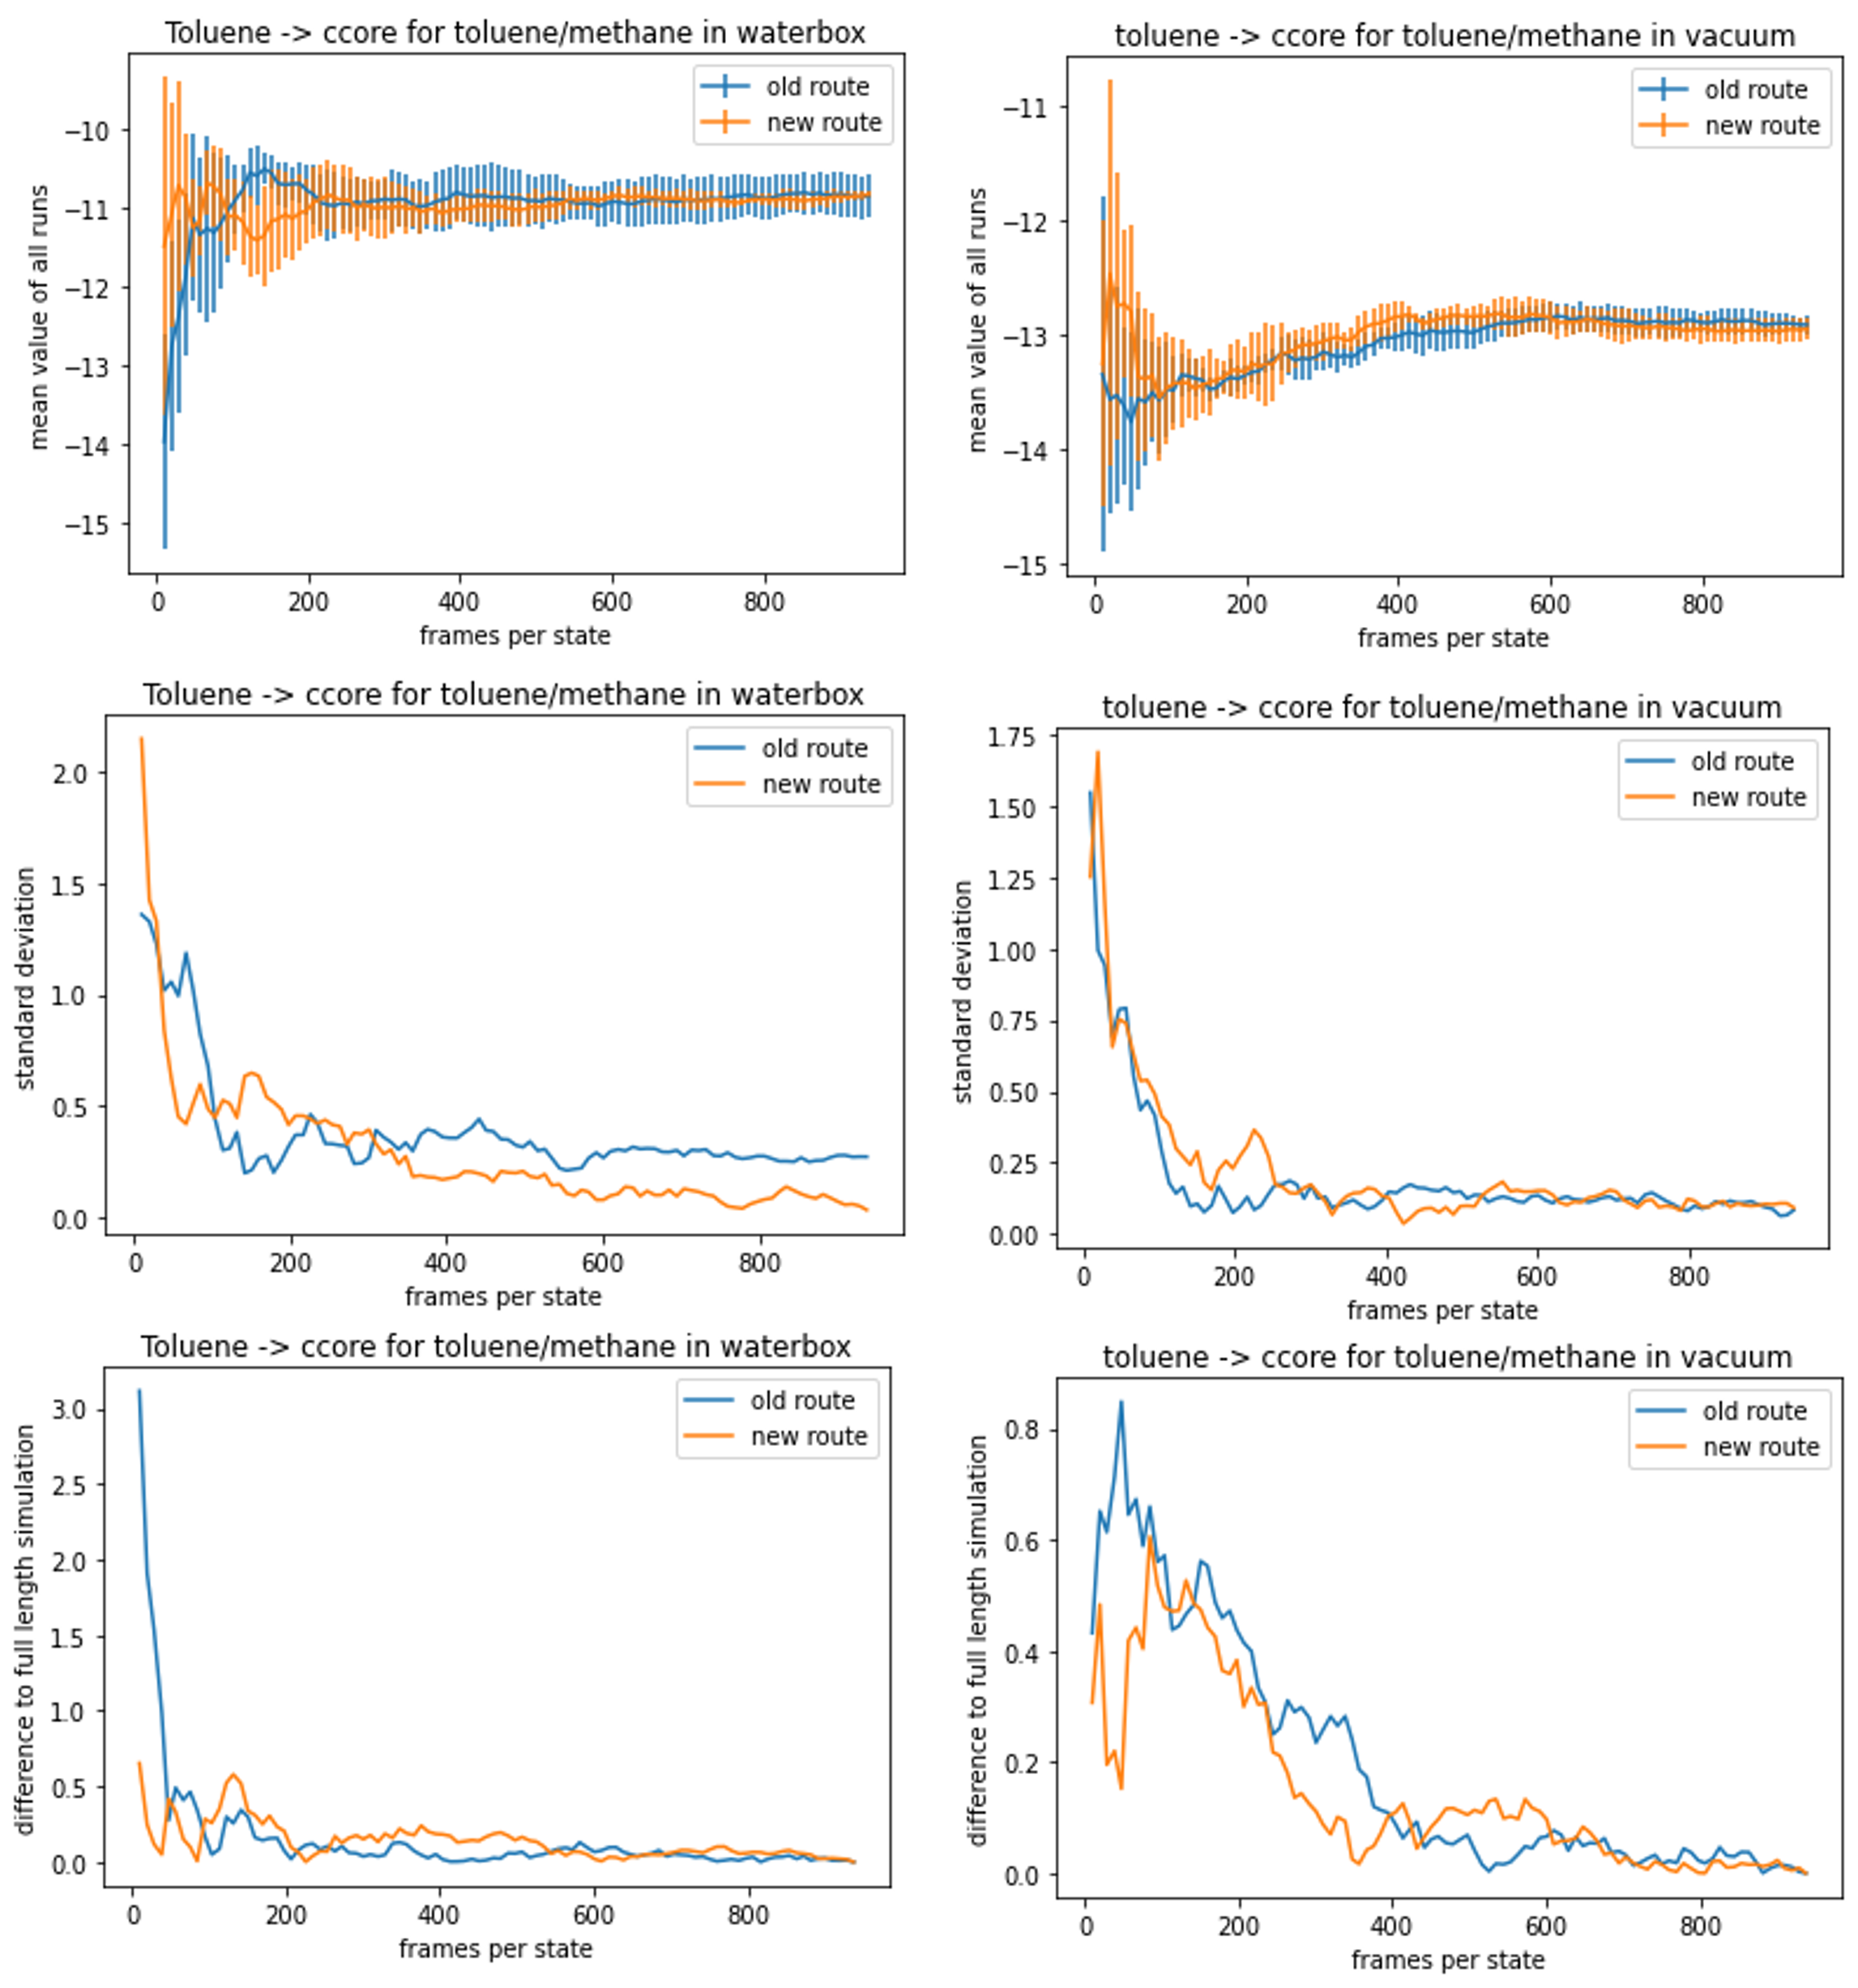
\includegraphics[scale=0.9]{toluene_short}\caption{toluene $\mathrm{\rightarrow}$ methane; left: water box; right: vacuum; mutation routes for toluene/methane; first row: mean value, bars indicate standard deviation; middle row: standard deviation; third row: difference to full-length simulation (i.e., the last value is zero)}
		\label{fig:toluene_short}
\end{figure}

\begin{figure}[!htb]
	
	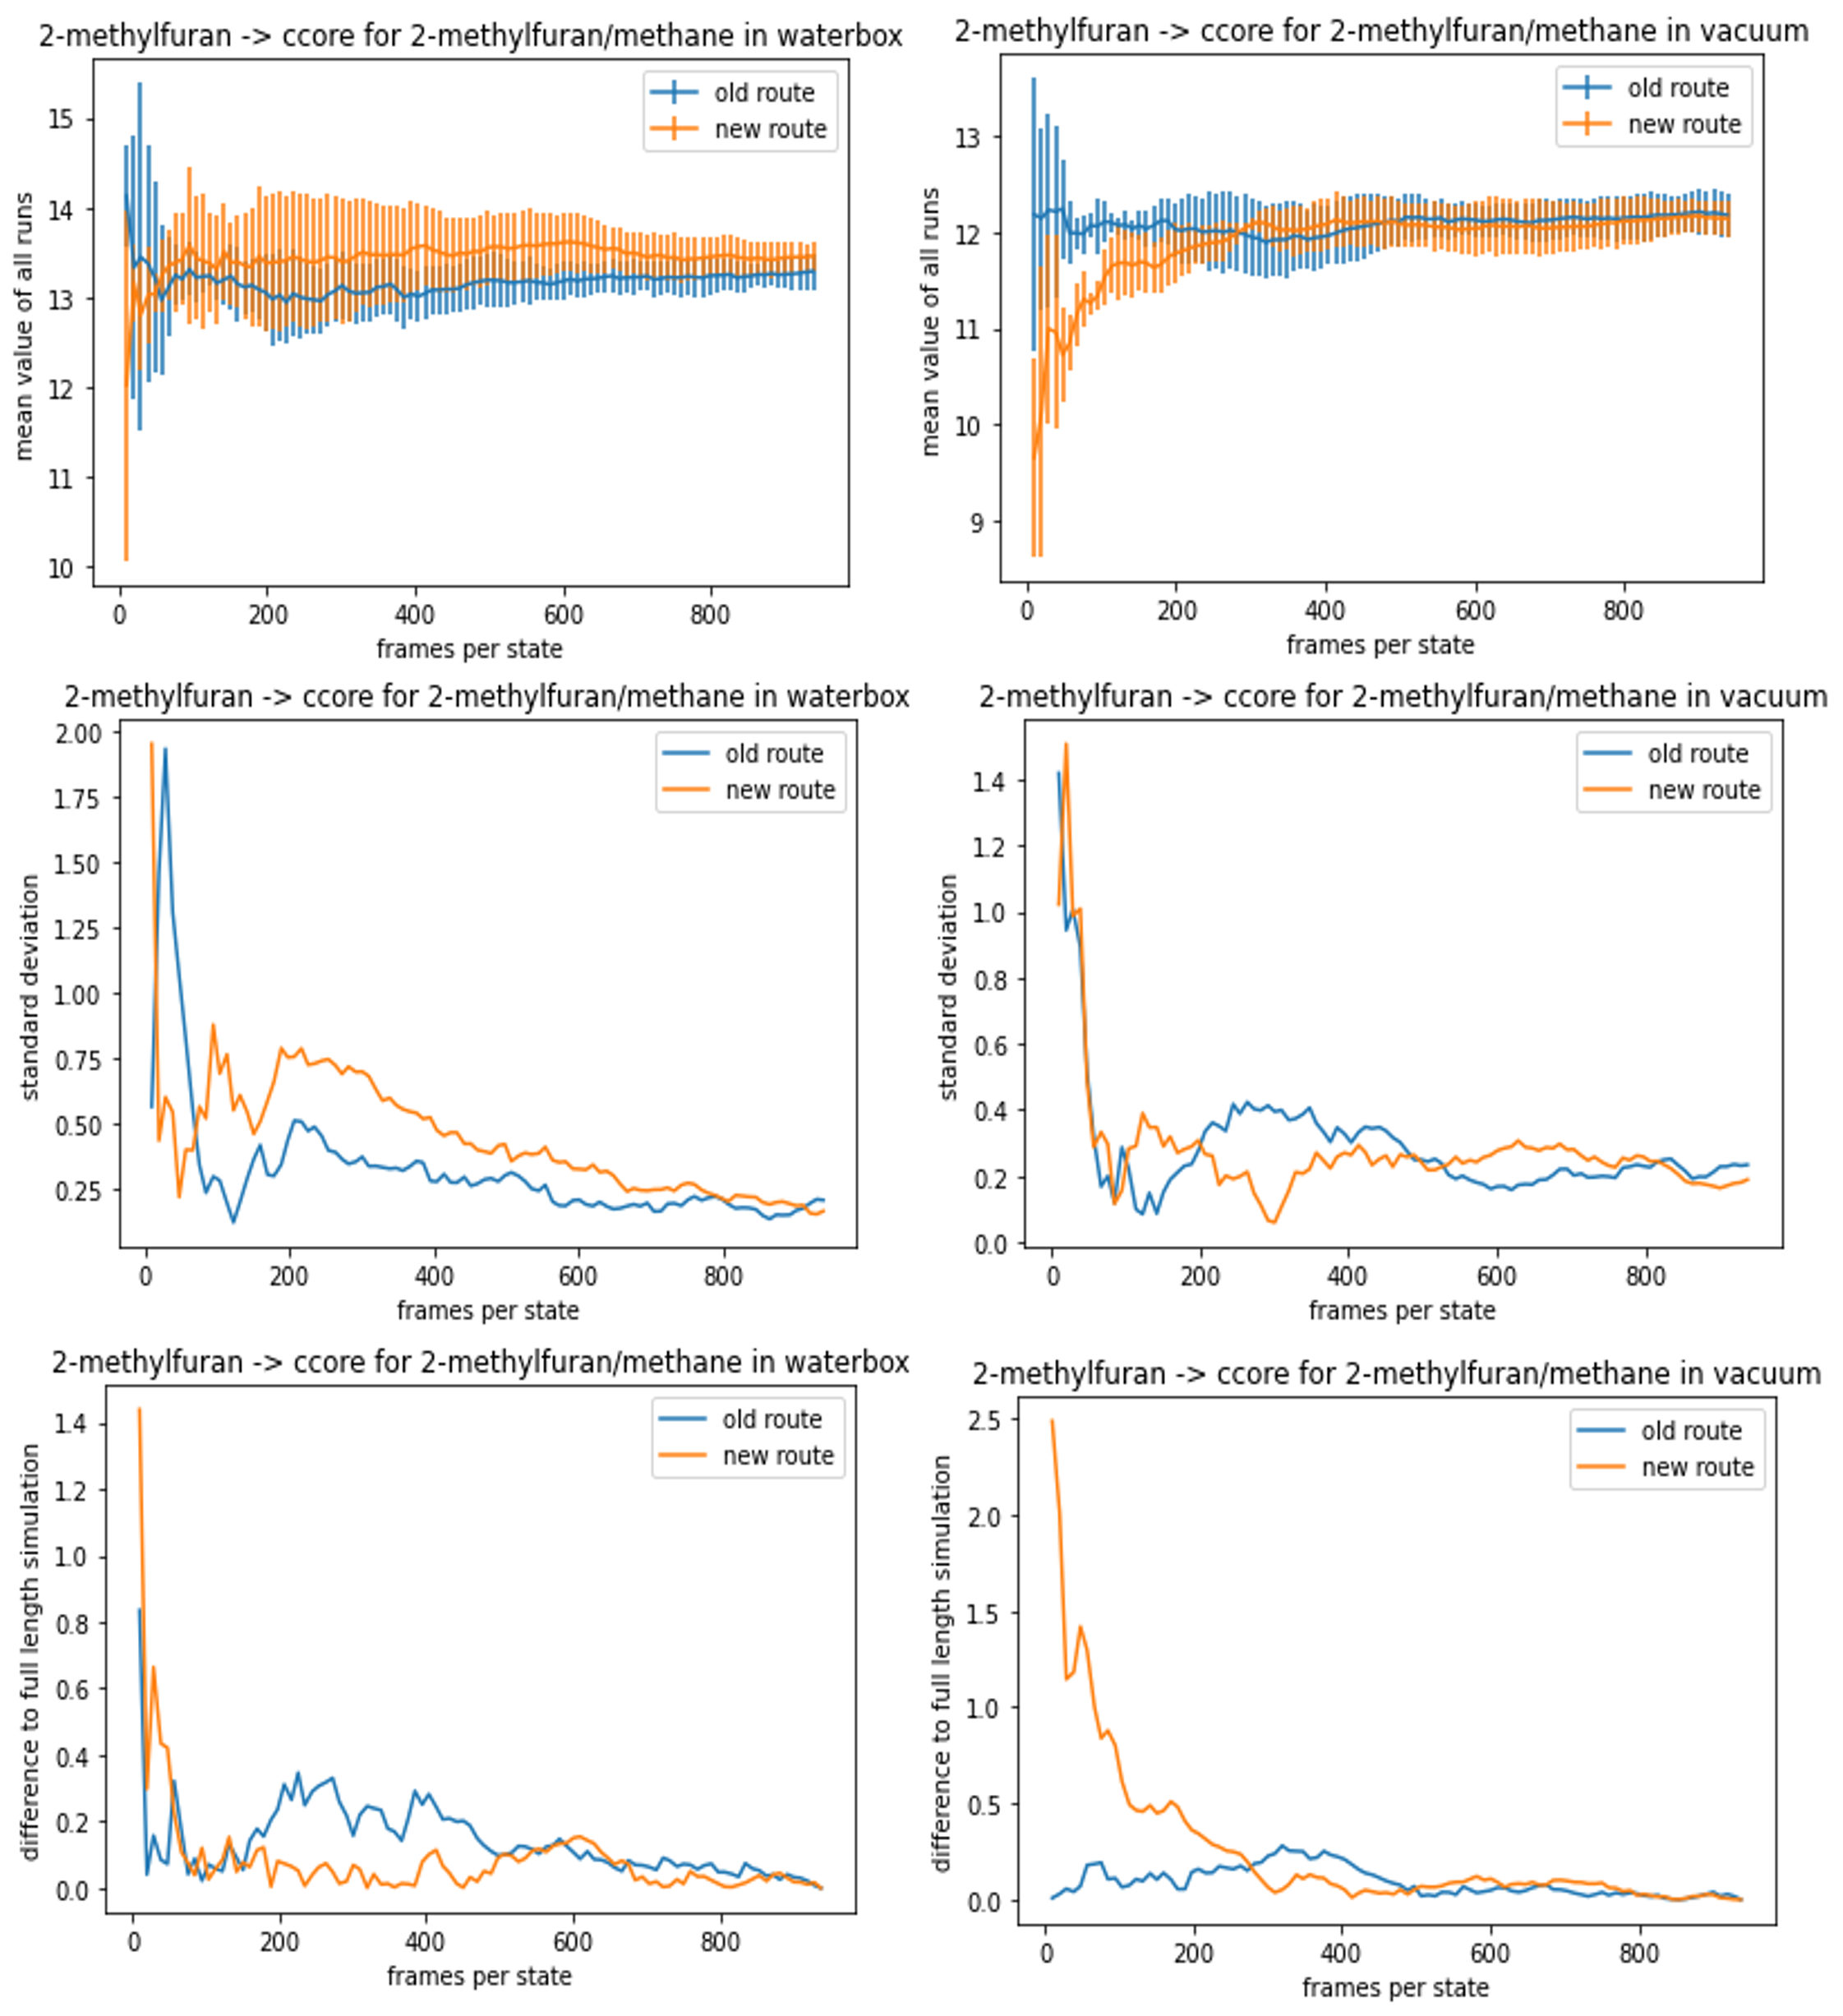
\includegraphics[scale=0.9]{methylfuran_short} \caption{2-methylfuran $\mathrm{\rightarrow}$ methane; left: water box; right: vacuum;  mutation routes for 2-methylfuran/methane; first row: mean value, bars indicate standard deviation; middle row: standard deviation; third row: difference to full-length simulation (i.e., the last value is zero)}
	\label{fig:methylfuran_short}
\end{figure}


\begin{figure}[!htb]
	
	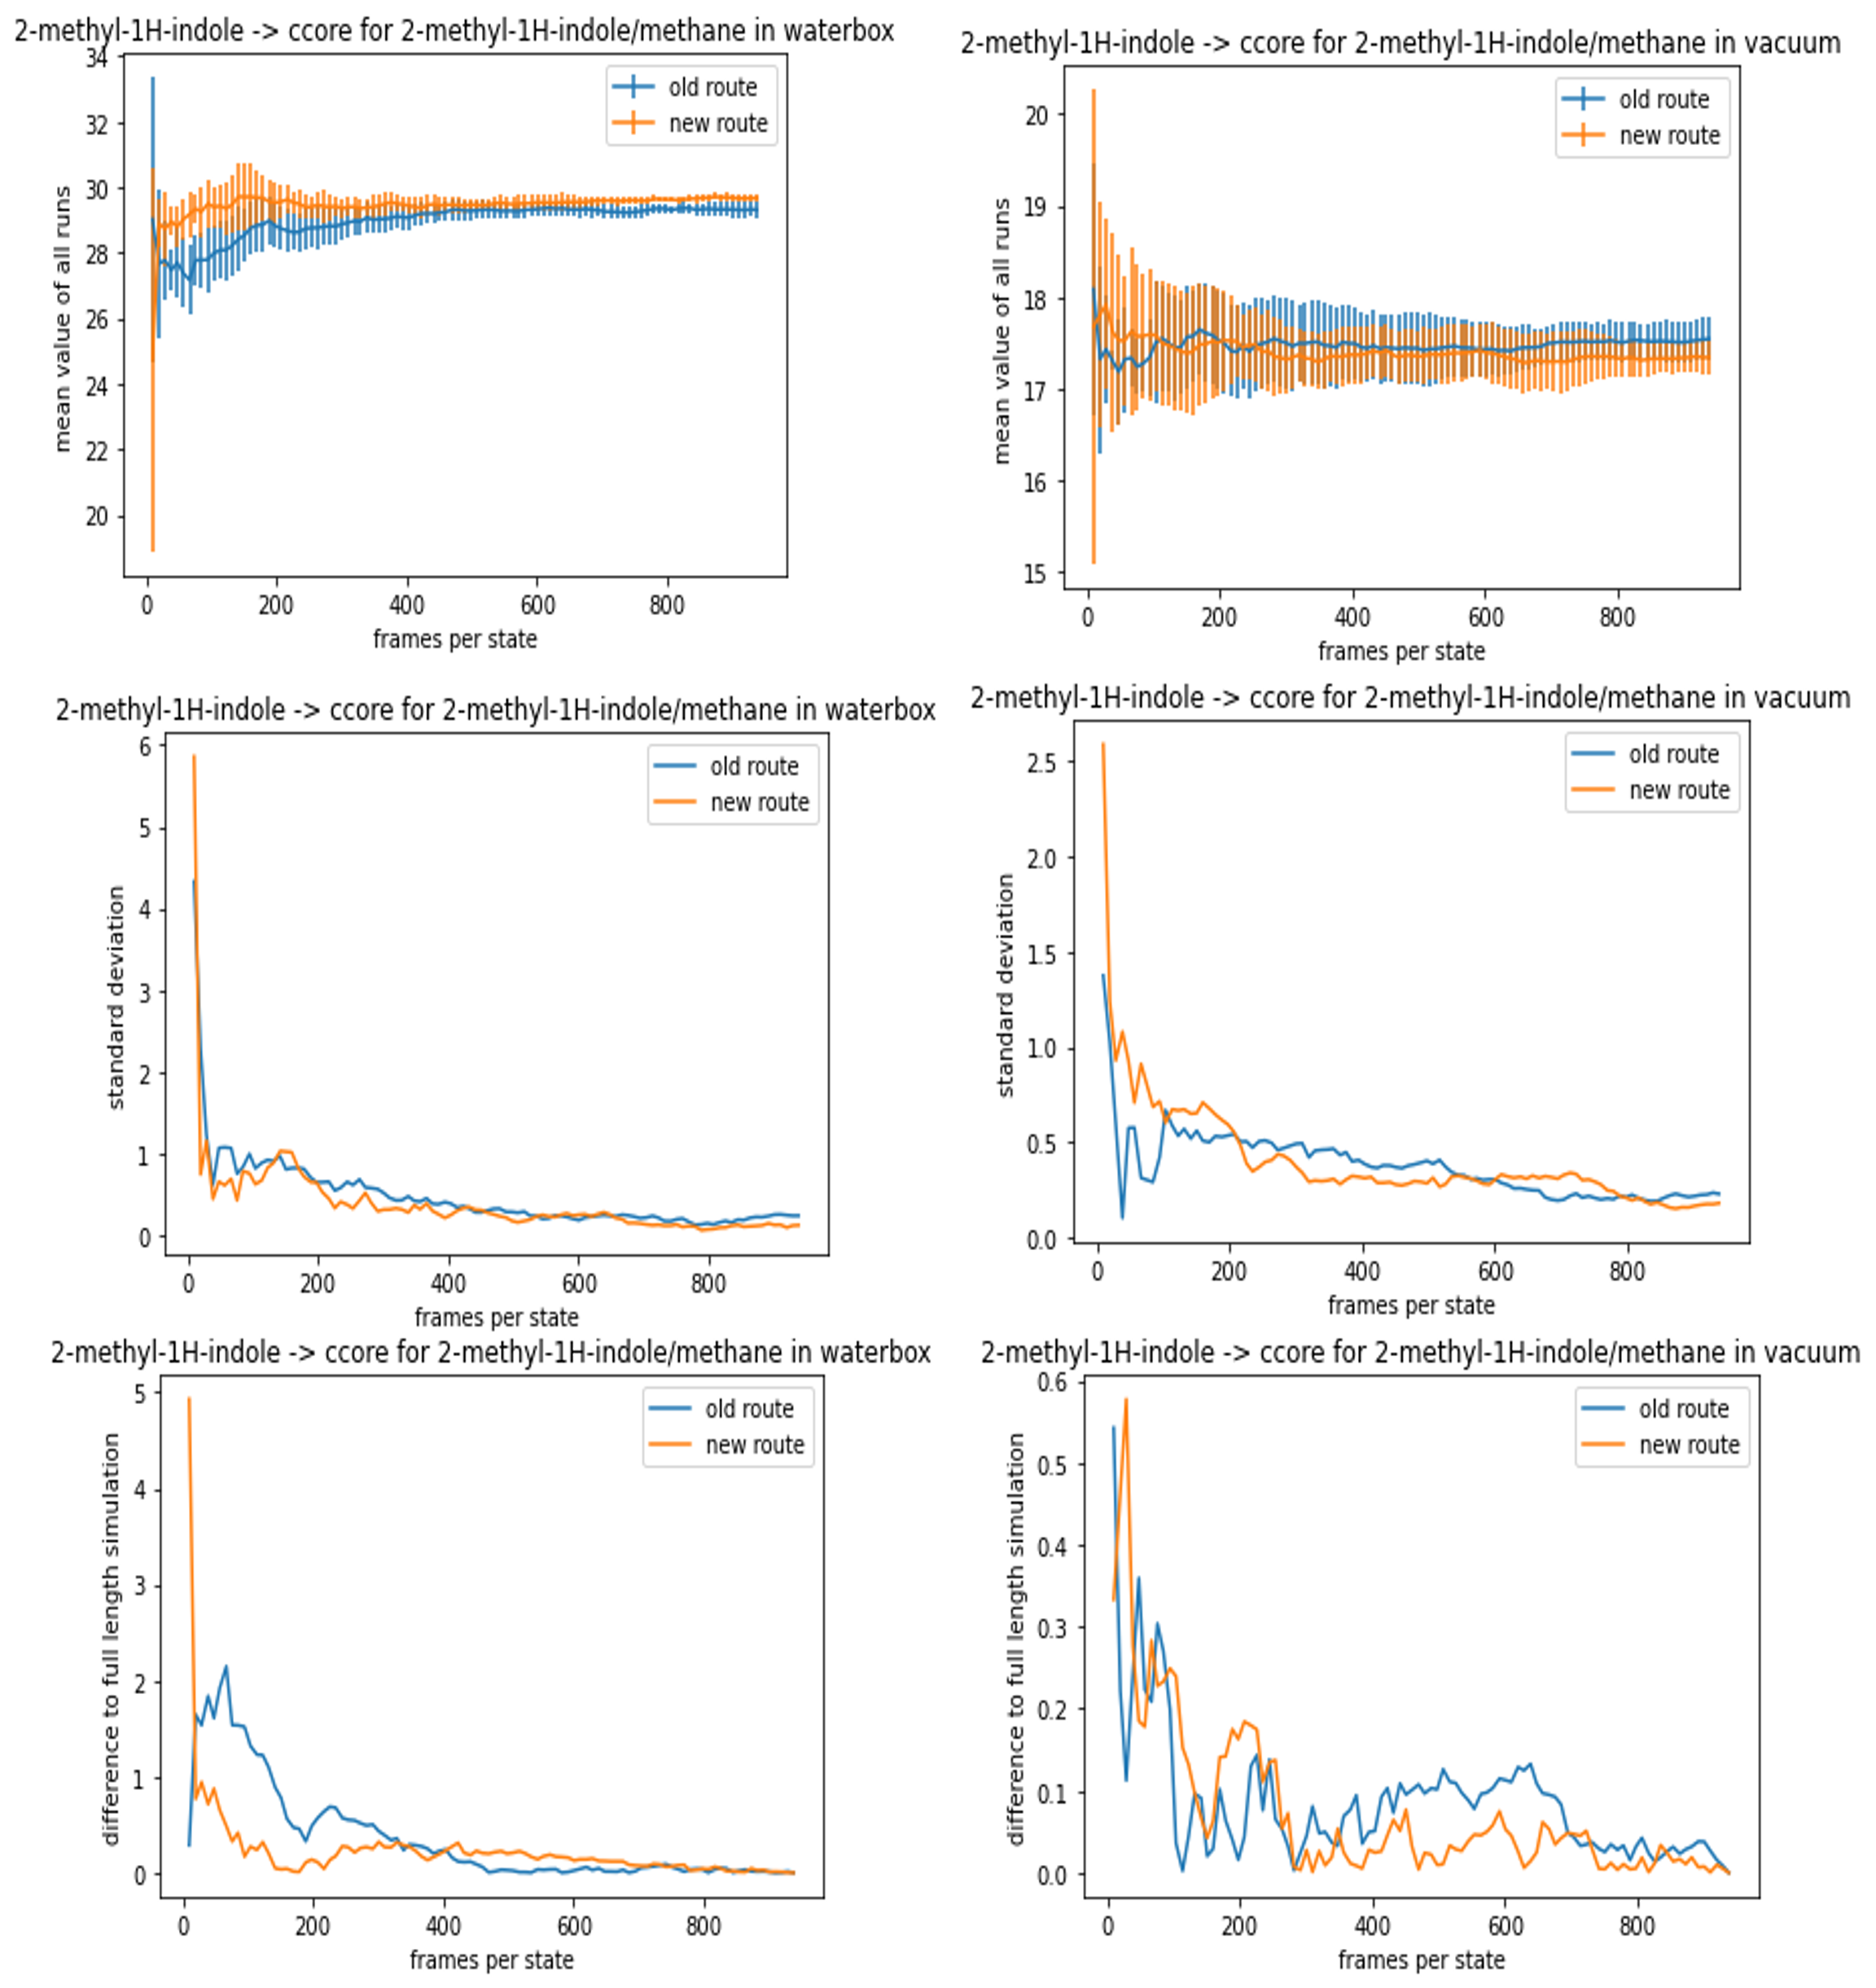
\includegraphics[scale=0.9]{methylindole_short}\caption{2-methylindole $\mathrm{\rightarrow}$ methane; left: water box; right: vacuum; mutation routes for 2-methylindole/methane; first row: mean value, bars indicate standard deviation; middle row: standard deviation; third row: difference to full-length simulation (i.e., the last value is zero)}
	\label{fig:methylindole_short}
\end{figure}

\begin{figure}[!htb]
	
	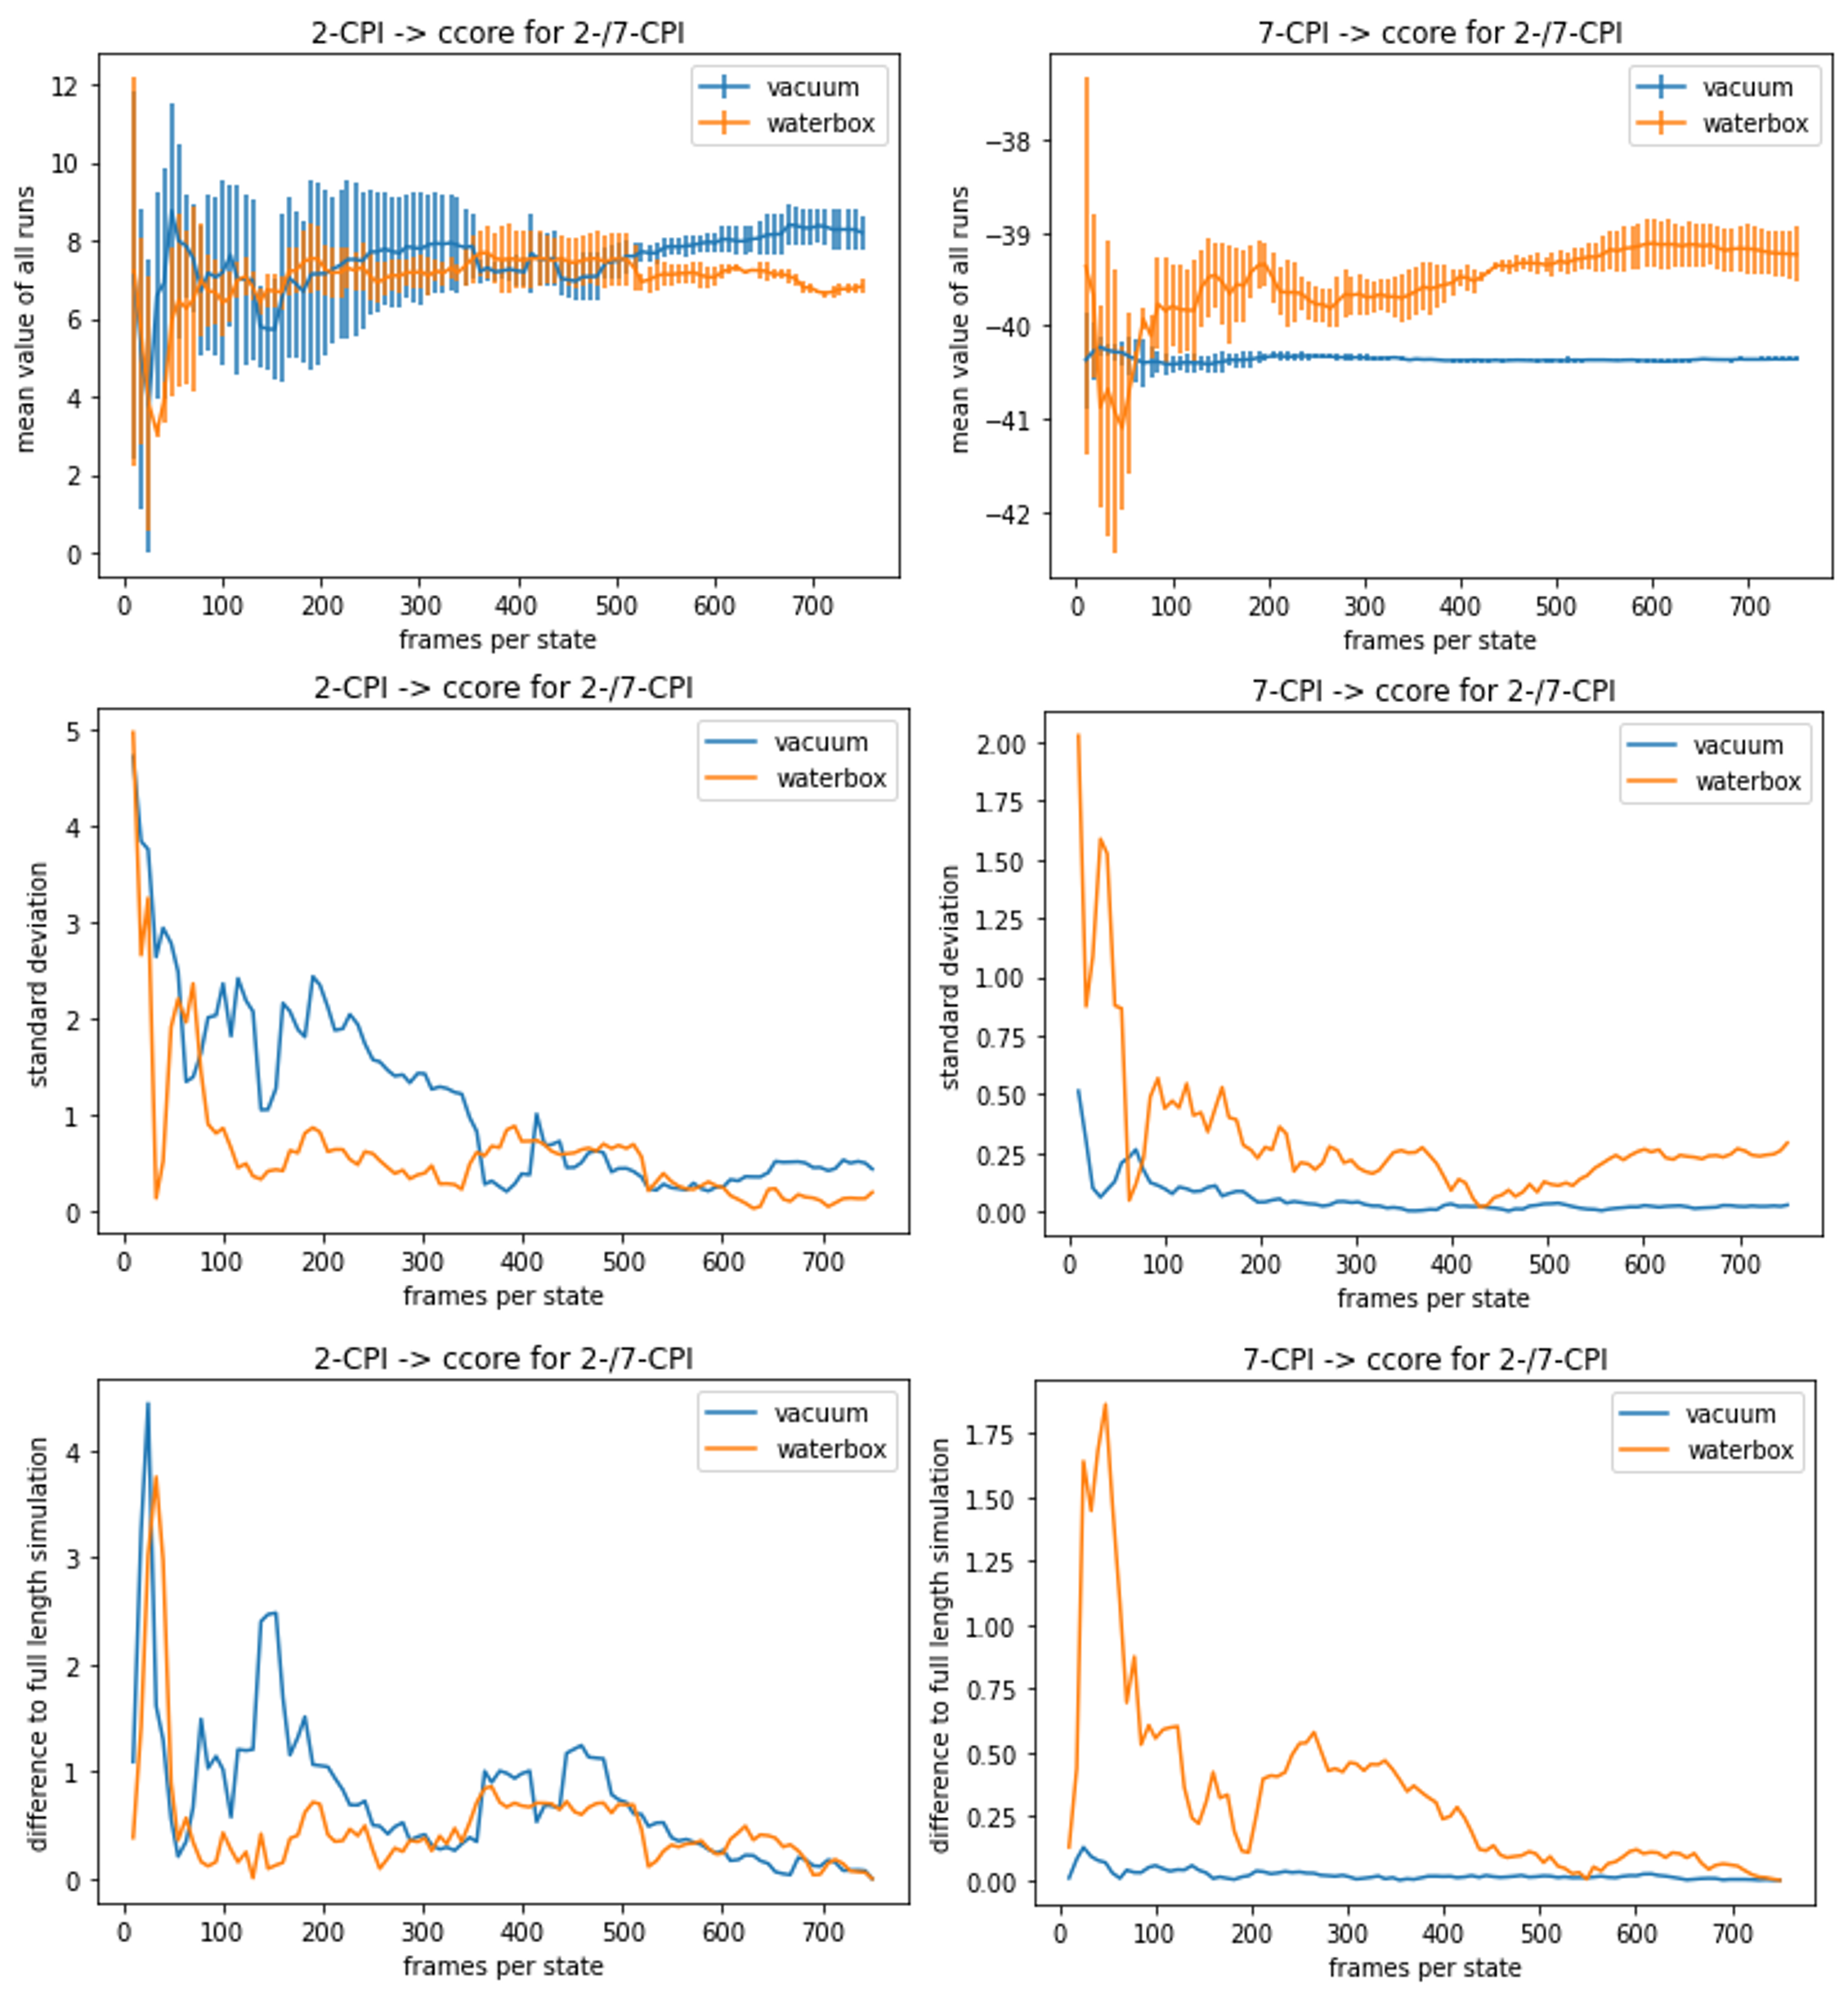
\includegraphics[scale=0.9]{cpi_short}\caption{left: 2-CPI $\mathrm{\rightarrow}$ CC for 2-/7-CPI; left: 7-CPI $\mathrm{\rightarrow}$ CC for 2-/7-CPI; first row: mean value, bars indicate standard deviation; middle row: standard deviation; third row: difference to full-length simulation (i.e., the last value is zero)}
	\label{fig:cpi_short}
\end{figure}

	\chapter{Conclusion}


Simulation results for the molecule pairs used in \cite{Loeffler.2018, Wieder.2022} suggest a superiority of the new mutation algorithms. For each molecule pair, the standard deviation of the new algorithms is smaller and for 2-/7-CPI the free energy difference is closer to the result of absolute free energy calculations. 
In this report, only rather small molecules and simple transformations have been carried out for test purposes. In any case, additional comparisons of mutation routes for other molecules and closer examination of the obtained results are necessary.

Especially for more complex transformations an evaluation of the relation between sampling length and standard deviation for different mutation routes could be insightful. 
It is possible that differences for such molecules are even more pronounced and choosing an algorithm which allows for shorter sampling size by minimizing variance could be efficient.

Perhaps also a more systematic evaluation of the emergence of differences between the mutation algorithms could use molecules with exactly defined, small modifications (for example, one added/removed atom or ring structure) to investigate if the size of the dummy regions or the common core and the combination of some elements, e.g. rings, have an effect. However, it should be stressed that in most cases the effects probably will be moderate and maybe not robust, i.e. below the standard error of the simulations.


The tf-routes package presented in this work also allows to process heavy non-carbon atoms in an individual manner, i.e. atoms of different types can be represented as nodes with different weight which impacts the mutation route. It would be interesting if there are more pronounced differences for molecules with such atoms.

However, in any case more results for molecules with different structure (e.g. different size and number of rings and chains, possible different atoms systems) and different sampling length would be necessary. The molecule pairs assessed so far are rather small and do not cover the space of possible structures at all.
Elucidating the apparently more complex and specific role between mutation order and resulting free energy differences could allow further improvement of the mutation route creation (given that the overall differences suggest that further optimization is expedient).

The greatest advantage of the new algorithms in comparison to the old versions is certainly that they should yield a correct common core and a 'reasonable' route for every molecule pair without exception (if a correct common core exists). In particular, the lack of special treatment of common core hydrogen atoms produced faulty common cores in previous versions of Transformato. The new processing always generates a valid common core with maximum atom size. Similarly, the old mutation route algorithm often led, especially in the case of bigger molecules, to atom removals in regions near the common core before chains etc. were systematically processed. Now both parts of the workflow, common core generation as well as mutation route determination are adjusted and should always yield reasonable outcomes.

    %\input{B) Chapters/00_using_the_template}
    %\input{B) Chapters/01_ordinary_text}
    %\input{B) Chapters/02_displayed_text}
    %\input{B) Chapters/03_tables_and_images}
    %\input{B) Chapters/04_code}
    %\input{B) Chapters/05_algorithms}
    %\input{B) Chapters/06_acronyms_and_glossary}
    %\input{B) Chapters/07_macros}
    %\listoftables 
    
    \listoffigures
    %\listofalgorithms
    
	%add your sources in the bib file and change the style here
    \bibliographystyle{alpha}
	\bibliography{bibliography}
	
	\printglossary[type=\acronymtype]
    \printglossary

    %\cleardoublepage{}
	%\pagebreak
	
	%add your end matter here
	%\appendix{}

	%\chapter{Appendix}

here you can put further things you want to add like transcripts, questionnaires, raw data...
	
	
	
\end{document}